\documentclass[utf8]{lgu}
\usepackage{listings}
\usepackage{booktabs}
\usepackage{array}
\usepackage[nopygments]{minted}
\usepackage{caption}
\usepackage{float}
\usepackage{graphicx}
\usepackage{needspace}
\usepackage{perpage}
\MakePerPage{footnote}
\usepackage[bottom]{footmisc}
\setlength{\footnotemargin}{1cm}
\renewcommand{\footnotelayout}{\hspace{0.5em}}
\floatstyle{plaintop}
\restylefloat{listing}
\providecommand{\theHlisting}{\thelisting}
\AtBeginEnvironment{listing}{\captionsetup{type=listing}}
\captionsetup[listing]{skip=10pt}

% Параметры для контроля размещения float-объектов
\setlength{\floatsep}{1pt plus 0pt minus 0pt}
\setlength{\textfloatsep}{2pt plus 0pt minus 0pt}
\setlength{\intextsep}{2pt plus 0pt minus 0pt}
\renewcommand{\floatpagefraction}{0.75}
\renewcommand{\textfraction}{0.15}
\renewcommand{\topfraction}{0.75}
\renewcommand{\bottomfraction}{0.35}

% Запрет висячих строк (widow/orphan control)
\widowpenalty=10000
\clubpenalty=10000

\AtBeginEnvironment{listing}{%
  \needspace{5\baselineskip}% Требуем минимум 5 строк свободного места
  \vspace{12pt}%
}
% Ensure exactly one normal first-line indent after listing
% Apply indent only to the very next paragraph after a listing
\AtEndEnvironment{listing}{\vspace*{-1pt}\par\everypar{\noindent\hspace*{\parindent}\everypar{}}}

% Команда для подписи листинга без изменения тегов/окружений
\makeatletter
\newcommand{\captionlisting}[1]{%
  \captionsetup{type=listing}%
  \captionof{listing}{#1}%
  \vspace{-11pt}%
}
\makeatother

% Запрещаем растягивание текста по вертикали
\raggedbottom

% Уменьшение отступа перед выравниваниями
\usepackage{etoolbox}
\BeforeBeginEnvironment{align}{\vspace{-10pt}}
\BeforeBeginEnvironment{align*}{\vspace{-10pt}}

% Увеличение отступа после таблиц
\AtEndEnvironment{table}{\vspace{10pt}}

%%% Info Dokumenta pirmajai & dokumentārajai lapai
\fakultate{Факультет инженерно\hspace{0.2ex}\raisebox{0.18ex}{-}технических наук}
\katedra{Кафедра информатики}
\nosaukums{Построение компилятора с~языка~программирования Оберон для~процессора~ARM64}
\darbaveids{Диссертация на соискание степени магистра} %dokumentarajai lapai
\DARBAVEIDS{Магистерская диссертация} 
\autors{Артур Игоревич ЕФИМОВ}
\studapl{aj24012}
\vaditajs{д-р техн. наук, проф. Карл Черан}
\recenzents{д-р Агрис Шостак}
\vieta{Рига}
\gads{2025}

%%% Valodu atbalsts ir stila failā, kur galvenā valoda - latviešu, bet te var pievienot papildu valodas
\setotherlanguages{english, latvian}
\frenchspacing
\PolyglossiaSetup{russian}{frenchspacing=true}

% Русское тире: узкие пробелы по бокам, слева — неразрывный.
% Использование: слово\tire другое.
\newcommand{\tire}{\unskip\nobreak\thinspace\textemdash\thinspace}

%%% Darbam noderīgas pakas
%\usepackage{mathtools}

%%% Глобальные настройки переносов и выравнивания текста %%%
% microtype: микротипографические улучшения (выступание знаков препинания за поля,
% лёгкое масштабирование шрифта для более равномерных пробелов)
\usepackage[protrusion=true, expansion=true, tracking=false]{microtype}

\sloppy                    % Разрешаем более широкие межсловные пробелы
\tolerance=3000            % Допуск к «плохим» строкам (по умолчанию 200)
\hbadness=3000             % Порог предупреждений об underfull/overfull
\emergencystretch=12em     % Дополнительная растяжка пробелов для узких полос A5
\hfuzz=2pt                 % Подавление мелких вылезаний (до 2pt)

% Настройки переносов: разрешаем переносить щедрее
\hyphenpenalty=50          % Штраф за перенос (по умолчанию 50, чем меньше — тем охотнее)
\exhyphenpenalty=50        % Штраф за перенос после явного дефиса
\doublehyphendemerits=5000 % Штраф за два переноса подряд (по умолчанию 10000)
\finalhyphendemerits=3000  % Штраф за перенос в предпоследней строке абзаца
\lefthyphenmin=2           % Минимум букв перед переносом
\righthyphenmin=2          % Минимум букв после переноса

\usepackage{float}
\usepackage{setspace}
 
%%% Te var pievienot matemātisko operatoru saīsnes
\DeclareMathOperator*{\argmax}{arg\,max}

%%% СНОСКИ
\usepackage[hang]{footmisc}
\setlength{\footnotemargin}{1.8em}
\makeatletter
\renewcommand{\@makefnmark}{\nnbsp\raisebox{0.6ex}{\fontsize{6pt}{6pt}\selectfont\thefootnote}}
\newcommand{\nnbsp}{{\spaceskip=0.3em\relax~}}

% Настройка линии над сносками: короче и больше места после неё
\renewcommand{\footnoterule}{%
  \kern-3pt
  \hrule width 0.25\textwidth height 0.4pt
  \kern 5pt
}
\makeatother

\usepackage{hyperref} %pdf hiperlinki un pareizi punkti. NEDZĒST!
\hypersetup{
    colorlinks=false,
    hidelinks
}
\renewcommand{\UrlFont}{\small\ttfamily}

% Подключаем свой шрифт для листингов
\setmonofont{ChertjozhA}[
    Path=fonts/,
    Extension=.ttf
]

\definecolor{bggray}{RGB}{245,245,245}
\definecolor{commentgray}{RGB}{120,120,120}
\definecolor{keywordblue}{RGB}{0,87,160}
\definecolor{stringbrown}{RGB}{180,90,0}
\definecolor{darkgray}{RGB}{50,50,50}

% Устанавливаем тёмно-серый цвет для всего текста
\AtBeginDocument{\color{darkgray}}

% Меньший шрифт для всех листингов minted
\setminted{fontsize=\footnotesize}

% Source code line numbers
\renewcommand{\theFancyVerbLine}{\textcolor[rgb]{0.5,0.5,0.5}{\footnotesize\arabic{FancyVerbLine}}}

\newminted[go]{go}{
  linenos,
  numbersep=8pt,
  fontsize=\normalsize,
  frame=lines,
  framesep=6pt,
  baselinestretch=1,
  style=bw,
  tabsize=2,
  breaklines=true,
  escapeinside=||,
  encoding=utf8,
  xleftmargin=0pt,
  xrightmargin=0pt,
  formatcom=\color{darkgray}
}

\newminted[modula2]{text}{
  linenos,
  numbersep=8pt,
  fontsize=\normalsize,
  frame=lines,
  framesep=6pt,
  style=bw,
  breaklines=true,
  escapeinside=||,
  encoding=utf8,
  xleftmargin=0pt,
  xrightmargin=0pt,
  texcomments=false,
  mathescape=false,
  commandchars=none,
  formatcom=\color{darkgray}
}

% Breakable variant for long Modula‑2 listings (no frame, can split across pages)
\newminted[modula2long]{text}{
  linenos,
  numbersep=8pt,
  fontsize=\normalsize,
  frame=lines,
  framesep=6pt,
  style=bw,
  breaklines=true,
  breakanywhere=true,
  encoding=utf8,
  xleftmargin=0pt,
  xrightmargin=0pt,
  texcomments=false,
  mathescape=false,
  commandchars=none,
  formatcom=\color{darkgray}
}

\newminted[pascal]{pascal}{
  linenos,
  numbersep=8pt,
  fontsize=\normalsize,
  frame=lines,
  framesep=6pt,
  style=bw,
  breaklines=true,
  escapeinside=||,
  encoding=utf8,
  xleftmargin=0pt,
  xrightmargin=0pt,
  formatcom=\color{darkgray}
}

\newminted[cc]{c}{
  linenos,
  numbersep=8pt,
  fontsize=\normalsize,
  frame=lines,
  framesep=6pt,
  style=bw,
  breaklines=true,
  escapeinside=||,
  encoding=utf8,
  xleftmargin=0pt,
  xrightmargin=0pt,
  formatcom=\color{darkgray}
}

\newminted[asm]{nasm}{
  linenos,
  numbersep=8pt,
  fontsize=\normalsize,
  frame=lines,
  framesep=6pt,
  style=bw,
  breaklines=true,
  escapeinside=||,
  encoding=utf8,
  xleftmargin=0pt,
  xrightmargin=0pt,
  formatcom=\color{darkgray}
}

\newminted[ebnf]{text}{
  linenos,
  numbersep=8pt,
  fontsize=\normalsize,
  frame=lines,
  framesep=6pt,
  style=bw,
  breaklines=true,
  escapeinside=@@,
  encoding=utf8,
  xleftmargin=0pt,
  xrightmargin=0pt,
  formatcom=\color{darkgray}
}

% Сохраняем базовый размер абзацного отступа и возвращаем его после листингов
\newlength{\savedparindent}
\AtBeginDocument{\setlength{\savedparindent}{\parindent}}

% Автовозврат красной строки после листингов minted/float
\newcommand{\restorefirstindent}{%
  \global\parindent=\savedparindent
  \global\everypar{\indent\global\everypar{}}}
\AfterEndEnvironment{modula2}{\restorefirstindent}
\AfterEndEnvironment{modula2long}{\restorefirstindent}
\AfterEndEnvironment{pascal}{\restorefirstindent}
\AfterEndEnvironment{cc}{\restorefirstindent}
\AfterEndEnvironment{go}{\restorefirstindent}
\AfterEndEnvironment{asm}{\restorefirstindent}
\AfterEndEnvironment{ebnf}{\restorefirstindent}
% В большинстве случаев листинги находятся внутри float `listing`, который сам гасит отступ;
% возвращаем красную строку уже после закрытия float'а
\AfterEndEnvironment{listing}{\restorefirstindent}

\setlength{\abovecaptionskip}{0pt}
\setlength{\belowcaptionskip}{0pt}

\DeclareCaptionLabelFormat{pirmkodslabel}{\textit{#1 #2.}}
\captionsetup[listing]{
  labelformat=pirmkodslabel,
  labelsep=space,
  labelfont=it,
  textfont=bf,
  name=Листинг,
  justification=raggedright,
  singlelinecheck=false
}

\newcommand{\code}[1]{{\normalsize\texttt{#1}}}
\newcommand{\codef}[1]{{\scriptsize\texttt{#1}}}


\newcounter{appsec}
\renewcommand{\theappsec}{\Asbuk{appsec}} % или \Alph{appsec}, если \Asbuk нет

\newcommand{\appsection}[1]{%
  \refstepcounter{appsec}%
  \section*{Приложение~\theappsec.\ #1}%
  \addcontentsline{toc}{section}{Приложение~\theappsec.\ #1}%
}

\begin{document}
{\color{black}\maketitle}
% Переопределяем формат номера страницы: маленький внизу, нормальный в ссылках
\makeatletter
\renewcommand{\thepage}{\arabic{page}}
\renewcommand{\ps@plain}{%
  \renewcommand{\@oddfoot}{\hfil{\scriptsize\thepage}\hfil}%
  \renewcommand{\@evenfoot}{\hfil{\scriptsize\thepage}\hfil}%
  \renewcommand{\@oddhead}{}%
  \renewcommand{\@evenhead}{}%
}
\pagestyle{plain}
\makeatother
\clearpage

% Дублирование титульной страницы + пустая страница
\edef\savedpg{\arabic{page}}%
{\color{black}\maketitle}%
\setcounter{page}{\savedpg}%


% Копия последней страницы («Бесплатно»)
\thispagestyle{empty}
\makeatletter
\vspace*{\fill}
\begin{center}%
  \hspace*{-3cm}
  \begin{minipage}{0.6\textwidth}
    \centering
    \scriptsize
    \textbf{Подписано к печати~ 30.01.26}

    \textbf{Бесплатно\;\;\,~ Рига. Латв.\;ССР}
  \end{minipage}
\end{center}
\makeatother
\newpage

\renewcommand{\contentsname}{\uppercase{Содержание}}
\makeatletter
\renewcommand{\tableofcontents}{%
  \section*{\centering\contentsname}%
  \@starttoc{toc}%
}
\makeatother
\tableofcontents

\newpage

\section*{Аннотация}
\addcontentsline{toc}{section}{Аннотация}
\firstparskip

Данная работа посвящена разработке компилятора языка программирования Оберон (последователя языка Паскаль), предназначенного для преобразования программ в машинный код современных процессоров. В качестве целевой платформы выбран процессор Apple Silicon (ARM64) под управлением операционной системы macOS.

Основной целью исследования является создание инструмента, позволяющего компилировать исходный код, написанный на языке Оберон, в объектный код, совместимый с современными процессорами архитектуры ARM64. В работе предусматривается рассмотрение и реализация всех основных этапов трансляции программного кода: от лексического и синтаксического анализа и проверки совместимости типов до генерации промежуточного представления, машинного кода и компоновки исполняемого файла. Особое внимание уделяется специфике архитектуры современных ARM64-процессоров и проблемам, связанным с адаптацией особенностей языка Оберон к низкоуровневой платформе. Также подчёркивается важность стиля и ясности исходного кода, поскольку сам компилятор разрабатывается на языке Оберон.

Итогом работы является функционирующий прототип компилятора, который может быть использован для дальнейшего развития и исследования потенциала языка Оберон в современных вычислительных системах.

\vspace{0.5cm}
\textbf{Ключевые слова:} компилятор, Оберон, Apple, ARM64, машинный код, Компонентный Паскаль.

\newpage

\section*{Abstract}
\begin{english}
\firstparskip

\textbf{Compiler Construction for the Language Oberon Targeting ARM64 Machine Code}
\vspace{0.5cm}

This thesis presents the design and implementation of a compiler for the Oberon programming language, a successor of Pascal, targeting modern processor architectures. The chosen platform is Apple Silicon (ARM64) running the macOS operating system.

The primary goal of this research is to develop a toolchain capable of translating Oberon source code into object code compatible with contemporary ARM64 processors. The work encompasses all major stages of compilation, including lexical and syntactic analysis, type checking, intermediate code generation, machine code emission, and executable linking. Particular emphasis is placed on addressing the architectural specifics of ARM64 and the challenges associated with adapting the high-level semantics of Oberon to a low-level execution environment. The clarity and structure of the source code are also highlighted, as the compiler itself is implemented in Oberon.

The outcome of this thesis is a functioning compiler prototype, providing a foundation for future development and further investigation into the applicability of the Oberon language in modern computing environments.

\vspace{0.5cm}
\textbf{Keywords:} compiler, Oberon, Apple, ARM64, machine code, Component Pascal.
\end{english}

\newpage

\section*{Anotācija}
\begin{latvian}
\firstparskip

\textbf{Kompilatora izveide Oberona valodai ARM64 procesora mašīnkodā}
\vspace{0.5cm}

Darbs ir veltīts programmēšanas valodas Oberons (Paskāļa sekotāja) kompilatora izstrādei, lai pārveidotu to par mūsdienu procesoru mašīnkodu. Izvēlētais procesors ir \textit{Apple Silicon} (ARM64) ar operētājsistēmu \textit{macOS}.

Pētījuma galvenais mērķis ir izveidot instrumentu, kas ļauj kompilēt Oberonā rakstīto pirmkodu objektkodā, kas ir saderīgs ar mūsdienu ARM64 arhitektūras procesoriem. Darbā paredzēts apskatīt un realizēt visus galvenos programmēšanas valodas tulkošanas posmus: sākot no leksiskās un sintaktiskās analīzes un tipu saderības pārbaudes līdz starpreprezentācijas koda un mašīnkoda ģenerēšanai un izpildāmā faila sastatīšanai. Īpaša uzmanība tiks pievērsta mūsdienu ARM64 arhitektūras procesora specifikai un problēmām, kas saistītas ar Oberona valodas īpašību pielāgošanu zema līmeņa platformai. Tāpat tiks uzsvērta pirmkoda stila un skaidrības nozīme, jo pats kompilators tiks rakstīts Oberona valodā.

Darba galarezultāts ir funkcionējošs kompilatora prototips, kuru varēs izmantot turpmākai attīstībai un Oberona valodas potenciāla izpētei mūsdienu skaitļošanas sistēmās.

\vspace{0.5cm}
\textbf{Atslēgas vārdi:} kompilators, Oberons, Apple, ARM64, mašīnkods, Komponentais Paskāls.
\end{latvian}

\newpage

\section*{Автореферат}
\addcontentsline{toc}{section}{Автореферат}
\firstparskip

\paragraph{Актуальность исследования.}

Язык программирования Оберон сочетает компактность, строгую типизацию и высокую систематичность, что обеспечивает надёжность и предсказуемость программ. Однако на платформе Apple Silicon (ARM64) нативный компилятор Оберона отсутствует, а существующие решения (трансляторы в Си или LLVM) не обеспечивают желаемой скорости компиляции и прозрачности преобразования программ. В связи с этим разработка нативного компилятора Оберона для архитектуры ARM64 является актуальной задачей.

\paragraph{Цель работы.}

Разработать прототип нативного компилятора, преобразующего исходный код на Обероне напрямую в машинный код ARM64 в формате Mach‑O под операционную систему macOS.

\needspace{8\baselineskip}
\paragraph{Научная новизна}

~

~

1.\hspace{0.5em}Создан прототип нативного компилятора с языка Оберон, непосредственно генерирующий машинный код ARM64 в формате Mach‑O без использования сторонних IR-фреймворков (LLVM) или генерации кода на Си.

2.\hspace{0.5em}Предложены методы адаптации высокоуровневых конструкций Оберона к особенностям Apple Silicon, включая правильную передачу вещественных параметров через VFP-регистры.

3.\hspace{0.5em}Реализована полная прозрачность процесса компиляции на современной вычислительной платформе: все этапы трансляции (лексика, синтаксис, семантика, промежуточное представление, кодогенерация, компоновка) доступны для изучения и модификации на том же языке программирования, который одновременно является и предметом компиляции.

4.\hspace{0.5em}Улучшена модульная архитектура компилятора по сравнению с существующими версиями.

5.\hspace{0.5em}Разработан компоновщик исполнимых файлов в формате Mach‑O.

\needspace{8\baselineskip}
\paragraph{Практическая значимость}

~

~

1.\hspace{0.5em}Разработанный инструмент может служить наглядным учебным материалом при освоении технологий построения компиляторов, а также машинного кода ARM64.

2.\hspace{0.5em}Компилятор готов к дальнейшему развитию и перенацеливанию на другие вычислительные системы, а исходные тексты\tire к включению в открытые образовательные и исследовательские проекты.

\paragraph{Структура работы.}

Работа состоит из введения, 13 глав, заключения, списка литературы и приложений. Основные главы посвящены предварительному анализу, описанию исходного языка, особенностям программирования на Обероне, проектированию и реализации всех этапов компиляции, адаптации к архитектуре ARM64 и формату Mach‑O.

\newpage
\phantomsection
\specnodala{Введение}

\firstparskip Язык программирования Оберон, разработанный Никлаусом Виртом~\cite{WirthOberon},\tire это компактный строго типизированный язык, предназначенный для создания как прикладных, так и системных программ. Он применяется при разработке операционных и встроенных систем, драйверов и компиляторов, а также поддерживает построение расширяемых объектно-ориен\-ти\-ро\-ван\-ных программных систем без нарушения строгой типизации~\cite{ETHOS}. Оберон зарекомендовал себя при разработке программно-аппаратных комплексов с повышенными требованиями к надёжности. Он нашёл применение в цифровых системах атомных электростанций~\cite{OberonAES} и электрораспределительных подстанций~\cite{OberonKaliningrad}, агропромышленном оборудовании~\cite{OberonAgro}, беспилотных летательных аппаратах~\cite{OberonBPLA1,OberonBPLA2}, железнодорожных и авиационных системах~\cite{OberonAvia} и даже в имплантируемых медицинских устройствах~\cite{Skulski,Astrobe,OberonRTS,OberonApplications}.

Благодаря лаконичному синтаксису и высокой степени систематичности\footnote{Систематичность языка Оберон обеспечивается, в частности, высокой степенью ортогональности его конструкций, т.~е. как правило, для каждой программной идеи существует один оптимальный способ выразить её. Из языка исключены избыточные и дублирующие элементы, оставлен только минимально необходимый набор.} язык применяется в образовательных проектах~\cite{OxfordOberon,WirthPIO,OberonCourses}. Строгая типизация, включая межмодульный контроль, способствует формированию у студентов профессионального стиля программирования. Дополнительным преимуществом является высокая скорость компиляции: для таких систем, как \textit{BlackBox Component Builder}~\cite{BlackBox,BlackBoxWiki}, время компиляции проектов из десятков тысяч строк кода измеряется миллисекундами.

Тем не менее, Оберон не получил столь же широкого распространения, как его предшественник Паскаль, что, по-видимому, связано не с техническими особенностями, а с коммерческими и маркетинговыми факторами. Вследствие этого количество полноценных компиляторов Оберона ограничено, а поддержка новых аппаратных платформ осуществляется эпизодически. Кроме того, существует проблема наличия нескольких не вполне совместимых диалектов языка, затрудняющих стандартизацию и развитие единой экосистемы.

Одна из таких новых аппаратных платформ\tire процессоры Apple Silicon, основанные на архитектуре ARM64. Для этой платформы нет нативного компилятора\footnote{Здесь и далее под нативным компилятором понимается компилятор, преобразующий исходный код на языке высокого уровня непосредственно в машинный код аппаратной платформы.} языка Оберон. Трансляторы Оберона в Си и другие промежуточные языки обладают тем существенным недостатком, что компиляция происходит медленно\tire то есть теряется одно из существенных преимуществ данного языка.

Таким образом, создание нативного компилятора языка Оберон для платформы Apple Silicon не только актуально, но и имеет стратегическое значение. Разработка такого компилятора позволит существенно повысить скорость компиляции программ на Обероне на устройствах с архитектурой ARM64, расширить применение языка в разработке современного программного обеспечения и предоставить научному и образовательному сообществу надёжный и перспективный инструмент. Кроме того, исходный код компилятора может быть использован в качестве наглядного приложения к учебным материалам по построению компиляторов.

Первый компилятор Оберона, совместно с одноимённой операционной системой и ЭВМ «Ceres» на базе процессора NS32000, был разработан Н.~Виртом в 1988---1990~гг. Последняя реализация в рамках «Проекта Оберон»~\cite{ProjectOberon1,ProjectOberon2} также принадлежит Вирту и создана в 2013---2016 гг. для специально разработанного RISC-процессора~\cite{WirthRISC}, функционирующего на ПЛИС (FPGA).

Целью данной работы является применение теории построения компиляторов, развитой в проекте Оберон (1988---2016)~\cite{WirthOberon}, к современной аппаратной платформе.

Для достижения поставленной цели необходимо решить следующие задачи:

1.\hspace{0.5em}Провести исследование существующих подходов и методов создания компиляторов языка Оберон, а также выявить их преимущества и недостатки с точки зрения использования на платформе Apple Silicon.

2.\hspace{0.5em}Проанализировать архитектурные особенности процессоров Apple Silicon с точки зрения генерации машинного кода, в том числе исследовать формат исполнимых файлов, использующийся на платформе macOS.

3.\hspace{0.5em}Спроектировать архитектуру нового компилятора: очертить круг его функционала и разбить его на программные модули, включая лексический и синтаксический анализаторы, систему учёта контекста, внутреннее представление кода, генерацию кода и компоновку (linking).

4.\hspace{0.5em}Реализовать модули лексического и синтаксического анализа языка Оберон, а также механизмы семантического анализа и проверки типов.

5.\hspace{0.5em}Разработать эффективные методы генерации нативного машинного кода для архитектуры ARM64.

6.\hspace{0.5em}Реализовать компоновщик (linker) или механизмы интеграции порождаемых компилятором объектных файлов в существующую систему сборки приложений macOS.

7.\hspace{0.5em}Провести испытания компилятора на примерах типовых задач, продемонстрировав таким образом корректность его работы.

8.\hspace{0.5em}Подготовить набор учебных примеров и рекомендаций по использованию компилятора.

Реализация поставленных задач позволит продемонстрировать потенциал языка Оберон на платформе macOS и станет значимым шагом на пути его интеграции в образовательную, научную и инженерную практику.

\section{Анализ на предварительном этапе}

\vspace{-6mm}

\firstparskip

\subsection{Текущие тенденции в компиляторостроении}

\firstparskip В современной практике построения компиляторов наблюдается всё более широкое использование готовых инструментов. Целью компилятора в сущности является перевод программы с одного языка на другой\tire с языка программирования высокого уровня в низкоуровневый машинный код. Эта цель определяет и два противоположных момента компилятора: \textit{препроцессор} (frontend), связанный с исходным кодом, и \textit{постпроцессор} (backend), связанный с целевой платформой. Даже если создатель компилятора не подразумевает явного разделения его на две указанные составные части, в нём всё равно с лёгкостью можно выделить эти противоположности: в виде разных наборов программных модулей, процедур или строк кода. Оба этих момента находят отражение в многообразии инструментов для решения задач компиляторостроения: с одной стороны, со стороны препроцессора, существуют генераторы лексических и синтаксических анализаторов. С~другой стороны, со стороны постпроцессора, существуют фреймворки, обеспечивающие генерацию машинного кода, такие как LLVM.

Утилита \code{re2c}\tire пример генератора \textit{лексического} анализатора~\cite{Re2c}. Она генерирует код на языке Си. Распространённым средством, позволяющим генерировать исходный код \textit{синтаксического} анализатора, является утилита Yacc. Более новый её аналог\tire GNU Bison\tire использован для создания синтаксического анализатора языка PHP~\cite{PhpBison}. В~качестве входных данных такие генераторы получают формальное описание синтаксиса, а на выходе мы имеем абстрактное синтаксическое дерево, готовое для обработки постпроцессором компилятора.

Готовые форматы промежуточных представлений и связанные с ними генераторы машинного кода, в том числе включающие в себя этап оптимизации, с одной стороны, позволяют сократить сроки разработки компилятора, с другой\tire порождают сложности при адаптации к специфическим целям. В~частности, для образовательных и исследовательских целей такой компилятор вряд ли подходит, ведь львиная доля его функционала скрыта в утилите-генераторе.

Одним из самых известных фреймворков компиляции является LLVM~\cite{LLVM}. Он предоставляет как промежуточное представление, так и набор инструментов для его оптимизации и генерации машинного кода. LLVM определяет собственную виртуальную архитектуру и язык ассемблера. Компиляторы, использующие LLVM, преобразуют исходный код в промежуточное представление LLVM, а затем используют инструменты LLVM для генерации кода под целевую платформу.

Это обеспечивает высокий уровень переиспользуемости и доступ к сложным оптимизациям. Однако, как показал опыт ряда проектов~\cite{LLVMBugs}, интеграция с LLVM может оказаться обременительной из-за:

1) высокой сложности API и документации;

2) большого объёма зависимостей и сборочной системы;

3) трудностей с отладкой IR и промежуточных фаз;

4) сравнительно низкой скорости на этапе генерации кода.

Для таких языков, как Оберон, где критически важна прозрачность всех этапов трансляции\footnote{Прозрачность компилятора приобретает особое значение в случае языков с минималистичным синтаксисом и строго определённой семантикой. Простота языка представляет собой самостоятельную ценность, выражающуюся в надёжности и предсказуемости вычислительного процесса: программист способен объять умом весь процесс компиляции и исполнения программы. Эта ценность легко нивелируется при использовании громоздких промежуточных этапов, таких как LLVM, скрывающих логику преобразования за слоями абстракции.}, интеграция с LLVM представляется избыточной и неоправданной. В~данной работе был сознательно выбран путь прямой генерации машинного кода без обращения к сторонним промежуточным представлениям. Такой подход позволил значительно упростить архитектуру компилятора, обеспечить полный контроль над структурой выходного файла и сделать все этапы трансляции доступными для понимания без наличия «чёрных ящиков».

Альтернативный путь\tire генерация кода на языке Си. Такой подход использовался, например, в компиляторах языков Эйфель, Модула-3 и некоторых реализациях Оберона. Язык Си в качестве промежуточного представления обеспечивает переносимость (хоть и с некоторыми оговорками), но оставляет разработчику лишь ограниченный контроль над машинными особенностями, затрудняет оптимизацию под конкретные архитектуры и замедляет процесс компиляции, ведь теперь в качестве завершающего этапа компиляции необходимо запускать компилятор Си.

При всей своей автоматизации генераторы вроде Yacc и Bison обладают рядом ограничений, делающих их непривлекательными для реализации компиляторов языка Оберон:

1.\hspace{0.5em}Язык изначально проектировался с учётом лёгкости разбора. Его грамматика идеально подходит для синтаксического анализа методом рекурсивного спуска\tire подхода, в котором каждый нетерминал грамматики реализуется как отдельная процедура, тело которой по определённым правилам выводится из описания этого нетерминала в РБНФ\footnote{РБНФ\tire расширенная Бэкус\tire Наурова форма (Extended Backus–Naur Form, EBNF).}.

2.\hspace{0.5em}Сделанный вручную синтаксический анализатор позволяет точно контролировать структуру и логику разбора, что особенно важно в образовательном или исследовательском контексте. Автоматически сгенерированный код Bison, напротив, зачастую содержит плохо читаемую структуру с множеством \code{goto}, переходов по состояниям и управляющих конструкций низкого уровня.

3.\hspace{0.5em}Как подробно показано в «Дисциплине программирования» Э.~Дейкстры~\cite{Discip}, обширное использование \code{goto} приводит к усложнению логики программы с точки зрения её структурности и к невероятному усложнению анализа корректности и верифицируемости такой программы. В~проектировании современных программ, и компиляторов в том числе, стремятся к чистому стилю, и поэтому не используют переходов \code{goto}, чтобы не нарушать предсказуемости потока управления программы.

Кроме того, если анализаторы и генераторы будут написаны самостоятельно, мы вольны выбирать язык программирования, на котором мы будем это делать. Логичным шагом представляется писать компилятор Оберона на самом Обероне. В~этом случае, изучая данную работу, будущие исследователи смогут изучить и «прочувствовать» язык Оберон в процессе чтения исходного кода компилятора, что устранит любое недопонимание характера и особенностей компилируемого языка.

\subsection{Актуальное состояние компиляторов языка Оберон и их архитектурная поддержка}

\firstparskip Поскольку целью настоящей работы является реализация компилятора языка Оберон с поддержкой платформы Apple Silicon, необходимо провести обзор существующих компиляторов Оберона, оценить их применимость, поддерживаемые архитектуры и модели исполнения. Особый интерес представляет наличие или отсутствие нативной поддержки архитектуры ARM64, а также уровень зрелости и юридическая доступность (лицензии) существующих решений.

Среди существующих компиляторов Оберона можно выделить следующие категории по способу генерации исполнимого кода:

1.\hspace{0.5em}\textbf{Нативные компиляторы}\tire генерируют машинный код напрямую, без промежуточных представлений (например, компилятор Project Oberon от Никлауса Вирта, предназначенный для архитектуры RISC5~\cite{WirthRISC}). Ни один компилятор Оберона нативно не поддерживает платформу ARM64. Поддержка других современных платформ также крайне ограничена.

2.\hspace{0.5em}\textbf{Компиляторы с генерацией кода на Си}\tire используют язык Си в качестве промежуточного представления. Получающийся код на Си затем компилируется стандартными средствами (GCC, Clang). Примерами могут служить системы Ofront~\cite{Ofront,OfrontGithub}, Ofront+~\cite{OfrontPlus,OfrontPlusETH}, CPFront~\cite{CPFront}, Vishap Oberon Compiler (VOC)~\cite{Voc, VocGithub}. Данный подход обеспечивает переносимость, но не даёт прямого контроля над особенностями целевой архитектуры, что критично для эффективной поддержки Apple Silicon. Кроме того, переносимость Си условна, так как для работы как самого компилятора, так и скомпилированных им программ, необходима библиотека времени исполнения, которую, как правило, приходится адаптировать к каждой новой платформе (Windows, Linux, BSD, macOS и др.).

3.\hspace{0.5em}\textbf{Компиляторы, использующие LLVM}\tire транслируют Оберон в промежуточное представление LLVM. Это позволяет получить поддержку многих платформ «из коробки», но требует интеграции с экосистемой LLVM. Пример\tire OBNC-LLVM (экспериментальный форк), либо исследовательские компиляторы.
  
4.\hspace{0.5em}\textbf{Интерпретаторы и виртуальные машины}\tire такие реализации, как OberonJS~\cite{OberonJS,OberonJSOnline} и Online Oberon~\cite{OberonOnline}, интерпретируют код или транслируют его в WebAssembly (WASM), что позволяет запускать приложения в браузере~\cite{ProjectOberonOnline}. Хотя это интересно с точки зрения переносимости, такие решения не подходят для задач, требующих низкоуровневого контроля над платформой.

5.\hspace{0.5em}\textbf{Компиляция в байткод других платформ (JVM, «.NET»)}\tire имеются попытки реализации компиляторов, генерирующих байткод Java~\cite{OberonNC} или «.NET»~\cite{GPCP}. Платформозависимые аспекты языка, в частности работа с памятью и модулями, затрудняют перенос Оберона в эти среды.

Особняком стоит компилятор МультиОберон~\cite{MultiOberon,MultiOberonGuide}, который имеет сразу три постпроцессора и способен транслировать исходную программу как в Си, так и в код LLVM, так и нативно в машинный код для некоторых платформ. Такое разнообразие объясняется нормативными требованиями к программному обеспечению для атомных электростанций. Приёмной комиссии должно быть продемонстрировано, что программа успешно компилируется различными компиляторами на различных вычислительных системах и, кроме того, работает одинаково. МультиОберон поддерживает следующие вычислительные системы:

1) Windows (x86);

2) Windows (x86\_64);

3) Linux (x86);

4) Linux (x86\_64);

5) Raspberry Pi (ARMv7l);

6) Ubuntu Linux (AArch64, 64-bit Raspberry Pi).

Кроме того, МультиОберон способен гибко изменять синтаксис входного языка. Для этого в нём были предусмотрены специальные синтаксические конструкции \code{USE} и \code{RESTRICT}~\cite{MultiOberonUseRestrict}.

Независимо от архитектуры или модели генерации кода, любая реализация компилятора требует наличия:

1) \textbf{библиотеки времени исполнения}\tire минимального набора функций, реализующих базовые возможности языка (работа со строками, ввод-вывод, сборка мусора при наличии и т.~д.);

2) \textbf{системной библиотеки модулей}\tire реализация базовых модулей стандарта языка (например, \code{In}, \code{Out}, \code{Files}, \code{Strings}).

Таким образом, хотя на сегодняшний день существует множество реализаций компиляторов Оберона, ни одна из них не предоставляет полноценной поддержки платформы Apple Silicon с нативной генерацией кода в формате Mach‑O. Это обосновывает актуальность настоящей работы, направленной на разработку такого компилятора.

Одним из доступных инструментов для компиляции программ на Обероне является интегрированная среда разработки Free Oberon~\cite{FreeOberonWeb}, автором которой является ваш покорный слуга. Free Oberon работает с помощью транслятора в Си Ofront+, содержит кроссплатформенный набор модулей, интегрированную среду разработки и удобный консольный компилятор с функцией автосборки проекта. К~моменту начала работы над данной работой Free Oberon поддерживал системы Windows и Linux. В~ходе работы автор портировал его также и на macOS.

\needspace{6\baselineskip}
\subsection{Подготовительный этап: раскрутка компилятора и исправление в Ofront+}

\firstparskip Поскольку разрабатываемый компилятор будет написан на том же языке, который он компилирует, возникает классическая задача раскрутки (bootstrapping): для начальной компиляции компилятора требуется уже существующий компилятор, способный транслировать код на Обероне. Пока создаваемый компилятор не станет достаточно зрелым, чтобы компилировать сам себя, необходимо использовать сторонний инструмент.

В качестве такого базового компилятора была выбрана система Free Oberon\tire кроссплатформенная среда разработки на языке Оберон, использующая в качестве промежуточного представления язык Си. Исходный код на Обероне преобразуется в эквивалентный код на языке Си с помощью транслятора Ofront+, после чего компилируется в машинный код стандартными средствами, такими как GCC или Clang. Это позволяет получать исполнимые файлы для широкого спектра архитектур, включая x86\_64 и ARM64.

На момент начала работы Free Oberon не имел поддержки macOS. Автор выполнил перенос системы на платформу macOS, используя версию для GNU/Linux в качестве основы. Основными задачами при портировании стали: адаптация системы сборки, в том числе самосборки системы Free Oberon, настройка компилятора Clang, а также обеспечение совместимости используемых библиотек и модулей языка с особенностями платформы Darwin.

В процессе портирования Free Oberon под macOS была выявлена ошибка в трансляторе Ofront+~\cite{OfrontPlusBug}, унаследованная от его предшественника Ofront. Ошибка проявлялась исключительно на архитектуре ARM64 (Apple Silicon) и заключалась в некорректной трансляции передачи параметров типа \code{REAL} (вещественных чисел) по значению при вызове процедур. При передаче значений других типов, а также при передаче параметров по ссылке (как параметры-переменные), ошибки не возникало. Также необходимым условием возникновения ошибки было то, что значение типа \code{REAL} должно быть полем записного типа, причём непременно неэкспортированным (приватным).

В ходе отладки оказалось, что правила ABI (Application Binary Interface) архитектуры ARM64 требуют передачи вещественных аргументов через регистры VFP (Vector Floating Point), тогда как целочисленные значения передаются через общие регистры. Транслятор Ofront+ не учитывал эту особенность, а именно: неэкспортированные поля записей вне зависимости от типа этих полей переводились на язык Си как массив типа \code{char}, который по размеру совпадал со спрятанными полями. Это работало для всех типов, кроме вещественных чисел, потому что массив типа \code{char} в действительности передавался процедуре точно так же, как, например, значение типа \code{int}. В~результате, сгенерированный Си-код нарушал соглашения о вызовах, приводя к ошибкам времени выполнения и неверным результатам вычислений.

Временное и довольно простое решение состояло в том, чтобы пометить поля типа \code{REAL} как экспортированные. Проведённый анализ и отладка позволили локализовать и устранить ошибку в Ofront+, после чего транслятор стал способен формировать корректно исполнимый код для платформы ARM64. Таким образом, и Free Oberon стал пригоден для использования в качестве исходного компилятора на платформе macOS с процессорами Apple Silicon.

\subsection{ARM64 как целевая архитектура}

\firstparskip Разрабатываемый компилятор нацелен на прямую генерацию машинного кода для архитектуры ARM64. Эта архитектура, официально обозначаемая как AArch64 (в соответствии со спецификацией ARMv8-A~\cite{ARMv8Manual}), представляет собой 64-битное расширение архитектуры ARM.

На момент написания работы архитектура ARM64 используется во всей современной линейке устройств Apple: от портативных и настольных ЭВМ (MacBook, Mac Mini, Mac Studio, iMac) до мобильных устройств (iPhone, iPad), а также встроенных платформ\tire Apple Watch (watchOS) и Apple TV (tvOS). Центральными процессорами этих устройств служат интегральные микросхемы Apple Silicon серий M и~A. Разработка, испытание и отладка разрабатываемого компилятора выполняются на ЭВМ «MacBook Pro» с процессором M3~Pro 2023~г. выпуска, а также на ЭВМ «MacBook Air» с процессором M1 2020~г. выпуска.

В операционной системе macOS основным форматом исполнимых файлов является Mach‑O (Mach Object)~\cite{MachOFormat}. Этот формат был разработан как часть микроядерной архитектуры Mach и используется в системах на базе ядра XNU, включая macOS, iOS, iPadOS и другие.

Mach‑O представляет собой модульный контейнерный формат, предназначенный для хранения машинного кода, данных, таблиц символов, информации для отладки и других метаданных, необходимых для корректного выполнения и сопровождения программ. Он поддерживает как статическую, так и динамическую компоновку, а также имеет встроенные механизмы для реализации безопасной загрузки, цифровой подписи и разметки сегментов памяти (таких как «\,\code{\_\_TEXT}\,» и «\,\code{\_\_DATA}\,»).

Аналогами Mach‑O в других операционных системах являются:

1.\hspace{0.5em}\code{ELF} (Executable and Linkable Format)\tire используется в Unix-подобных системах, включая Linux и BSD. Это наиболее распространённый формат исполнимых файлов в мире открытого программного обеспечения.

2.\hspace{0.5em}\code{PE} (Portable Executable)\tire применяется в операционных системах семейства Windows. Основан на формате \code{COFF}, но дополнен структурами, специфичными для Windows. Исполнимые файлы имеют расширение \code{EXE} и начинаются со специальной заглушки (stub)\tire заголовка MS-DOS в формате \code{MZ}~\cite[с.~8]{Win32PE}.

3.\hspace{0.5em}\code{COFF} (Common Object File Format)\tire формат использовался в операционной системе Unix System~V.

4.\hspace{0.5em}\code{A.out}\tire старейший формат исполнимых файлов в Unix-системах, ныне практически не используется.

5.\hspace{0.5em}\code{NE} (New Executable) и \code{LE} (Linear Executable)\tire устарев\-шие форматы, использовавшиеся в ранних версиях Windows и OS/2.

6.\hspace{0.5em}\code{MZ} (DOS Executable)\tire используется в MS-DOS и Free\-DOS. Один из первых широко распространённых форматов, известный по сигнатуре \code{MZ} в заголовке. Послужил основой для \code{NE} и \code{PE}.

Бинарный формат Mach‑O используется не только для исполнимых файлов, но и для:

а) динамически подключаемых библиотек (dylib);

б) объектных файлов (object files, «\,\code{.o}\,»);

в) статических библиотек (archives, «\,\code{.a}\,»);

г) плагинов приложений;

д) модулей ядра и расширений системы;

е) тестовых и отладочных сборок.

Mach‑O\tire универсальный формат представления машинного кода в среде macOS. Его поддержка в компиляторе обязательна для интеграции с экосистемой Apple, в частности с системным загрузчиком.

В рамках данной работы компилятор генерирует исполнимые файлы напрямую в формате Mach‑O, минуя промежуточные слои вроде LLVM или GCC. Это требует как детального понимания внутренней структуры формата, так и правил вызова (ABI) и соглашений о размещении кода и данных в памяти~\cite{AppleSecurity}. Поэтому помимо обращения к официальной документации, выполнено и экспериментальное исследование файлов-образцов формата Mach‑O: как с применением специальных утилит, так и и на уровне шестнадцатеричного кода\footnote{См. гл.~\ref{sec:MachOExperiment} на с.~\pageref{sec:MachOExperiment} настоящей работы.}.

\section{Исходный язык}

\firstparskip В качестве исходного языка для разрабатываемого компилятора выбран Оберон~\cite{Oberon07Report}. Данный язык представляет собой результат последовательной эволюции языков структурного программирования, начатой с языка Алгол (1960), продолженной в Паскале (1970) и Модуле‑2 (1980) и достигшей логического завершения в Обероне (1990).

Язык Оберон разработан профессором Никлаусом Виртом в Швейцарской высшей технической школе (ETH Zürich) как упрощённый и концептуально более целостный преемник языка Модула‑2. Основной целью его создания являлось достижение максимальной выразительности при минимальной сложности синтаксиса и семантики. Важнейшим принципом при проектировании языка стала ориентация на простоту, ортогональность конструкций языка и минимализм, обеспечивающие как удобство практического программирования, так и простоту построения компиляторов.

Эволюционная цепочка «\,Алгол\,$\rightarrow$\,Паскаль\,$\rightarrow$\,Модула‑2\,$\rightarrow$\,\allowbreak Оберон\,» демонстрирует движение в сторону упрощения языковых конструкций при одновременном сохранении (а~в ряде случаев и расширении) выразительных возможностей. Оберон отличается строгой модульной структурой, статической типизацией и расширяемостью записных типов.

\subsection{Диалекты языка Оберон}

\subsubsection{Оберон (1990)}

\firstparskip Язык Оберон существует в нескольких диалектах. Оригинальная версия, разработанная в конце 1980-х годов, отличается от последующих, в частности, отсутствием цикла \code{FOR}. Эта конструкция была сознательно исключена: предполагалось, что она избыточна, ведь её функциональность может быть реализована с помощью цикла \code{WHILE}. Во всех других диалектах Оберона цикл \code{FOR} присутствует.

\needspace{6\baselineskip}
\subsubsection{Оберон‑2}

\label{Oberon2}

\firstparskip Оберон‑2, появившийся в 1991, возвращает в язык цикл \code{FOR}, а также делает существенное дополнение\tire возможность объявления процедур, связанных с записным типом (type-bound procedures). При объявлении процедуры перед её названием в скобках указывается \textit{приёмник}\tire переменная записного типа (см. код \ref{lst:TypeBound}), которая является функциональным аналогом ключевого слова \code{this} или \code{self} в других языках программирования. Примечательно, что в языке Го (2009) используется в точности тот же синтаксис.

Такие процедуры могут перегружаться в типах-расширениях, что напоминает виртуальные методы языка C++. Также в языке Оберон‑2 добавлена возможность помечать переменные и поля записей знаком «\code{-}», что обеспечивает их экспорт только для чтения.

\vspace{2.5\baselineskip}
\captionsetup{type=listing}
\captionlisting{Связанные с типом процедуры в Обероне‑2}
\label{lst:TypeBound}
\begin{modula2long}
MODULE TypeBoundExample;

TYPE
  Rectangle = RECORD
    a-, b-: REAL
  END;

PROCEDURE InitRectangle(VAR r: Rectangle; a, b: REAL);
BEGIN
  r.a := a;
  r.b := b
END InitRectangle;

PROCEDURE (r: Rectangle) Square(): REAL;       (* Здесь r — приёмник *)
BEGIN
  RETURN r.a * r.b
END Square;

PROCEDURE (VAR r: Rectangle) SetSize(a, b: REAL);          (* и здесь *)
BEGIN
  r.a := a;
  r.b := b
END SetSize;

PROCEDURE Do*;
VAR r: Rectangle;
  x: REAL;
BEGIN
  InitRectangle(r, 4, 7);
  x := r.Square();
  r.SetSize(5, 6)
END Do;

END TypeBoundExample.
\end{modula2long}

\subsubsection{Компонентный Паскаль}

\firstparskip Компонентный Паскаль представляет собой ещё один диалект языка Оберон. Изменения по сравнению с Обероном‑2 минимальны и касаются в основном введения новых возможностей для более строгой типизации и описания интерфейсов. В~частности, добавлены специальные атрибуты для типов и методов: \code{ABSTRACT}, \code{EXTENSIBLE}, \code{LIMITED} и \code{EMPTY}~\cite{ComponentPascalReport}.

Также была расширена работа со строками: появилась возможность сцепления строк с использованием оператора~«\,\code{+}\,», а также поддержка операций копирования строк до нуль-терминатора\footnote{Под нуль-терминатором понимается литера с кодом 0, обозначающий конец строки.}. 

Компонентный Паскаль также допускает определять в модуле секцию \code{CLOSE}. Последовательность операторов в этой секции будет выполнена при выгрузке модуля из ОЗУ.

\vspace{1.3\baselineskip}
\captionsetup{type=listing}
\captionlisting{Секция CLOSE в Компонентном Паскале}
\label{lst:ComponentPascalClose}
\begin{modula2long}
MODULE ExamplesClose;
IMPORT Log;
BEGIN
  Log.String('Hello'); Log.Ln
CLOSE
  Log.String('Good bye'); Log.Ln
END ExamplesClose.
\end{modula2long}

\needspace{8\baselineskip}
\subsubsection{Пересмотренный Оберон (Оберон-07)}

\label{sec:Oberon07}

\firstparskip Несмотря на участие в создании языка Оберон‑2, Никлаус Вирт в дальнейшем пришёл к выводу, что многие из нововведений оказались избыточными и усложняли исходную концепцию языка. В~2007 году он вернулся к первой версии языка Оберон и выпустил пересмотренную спецификацию, получившую неофициальное название Оберон-07. Эта редакция основана на оригинальном Обероне 1990 года, но содержит ряд уточнений и упрощений, направленных на повышение строгости и однозначности языка.

Ключевым отличием Оберона-07 от Оберона‑2 является отказ от процедур, связанных с типами (type-bound procedures), а также упрощение и уточнение ряда синтаксических конструкций. Если в оригинальном Обероне и Обероне‑2 тип \code{POINTER} мог указывать как на запись, так и на массив, то в Обероне-07 указатели разрешены исключительно на записи. Это убирает из языка поддержку динамических массивов.

С целью исключения использования типа \code{CHAR} не по назначению в низкоуровневых задачах в язык был добавлен совместимый с \code{INTEGER} базовый тип \code{BYTE}. Также устранено неявное преобразование из \code{INTEGER} в \code{REAL}: теперь приведение типов осуществляется явно с помощью встроенной функции \code{FLT}.

Синтаксическая конструкция \code{WITH}, использовавшаяся ранее для работы с переменными динамического типа, была исключена. Её функциональность теперь реализована конструкцией \code{CASE}, которая до этого использовалась только с числовыми переменными. Из оператора \code{CASE} была убрана ветвь \code{ELSE}\tire таким образом, невозможность выбрать ветвь приводит к аварийному останову.

Оператор цикла \code{WHILE} теперь поддерживает ветви \code{ELSIF}~\ldots~\code{DO}, что превращает его в оператор цикла Дейкстры. Убран оператор «бесконечного» цикла (цикла с выходом из середины) \code{LOOP}, а вместе с ним убран и оператор \code{EXIT}.

Упрощена семантика цикла \code{FOR}: теперь он определён через цикл \code{WHILE}, что устраняет возможные неоднозначности, связанные с граничными значениями диапазона управляющей переменной цикла, т.~е. при целочисленном переполнении.

Возврат из процедуры теперь разрешён только в её конце (см. подробнее на с.~\pageref{sec:Oberon07Return}).

Передача параметров массивов и записей по значению осуществляется в режиме только для чтения, что позволяет избежать лишнего копирования данных и повышает безопасность.

Строковые литералы обозначаются только двойными кавычками «\,\code{"}\,». Обозначать их одинарными кавычками (апострофами, «\,\code{'}\,») в Пересмотренном Обероне нельзя.

Последняя версия спецификации языка датируется 2016 годом и опубликована под названием «The Programming Language Oberon»~\cite{Oberon07Report}.

\subsubsection{Пересмотренный Оберон‑2}

\firstparskip Интересной ветвью развития языка является Пересмотренный Оберон‑2 (Revised Oberon-2), представленный в 2020 году Андреасом Пирклбауэром~\cite{RevisedOberon2Report}. В~отличие от оригинального Оберона‑2\footnote{См. с.~\pageref{Oberon2} настоящей работы.}, который был надмножеством Оберона 1990 года и добавлял, среди прочего, процедуры, связанные с типами (type-bound procedures), новая версия основывается на Пересмотренном Обероне (Обероне-07) и аналогичным образом расширяет его функциональность.

Кроме того, Пересмотренный Оберон‑2 вводит в язык Оберон образца 2016 года (Оберон-07) следующие средства:

1.\hspace{0.5em}\textbf{Процедура динамического выделения памяти в куче для массивов фиксированной длины и открытых массивов.} Во всех диалектах Оберона предусмотрена стандартная процедура \code{NEW}, предназначенная для динамического распределения памяти, в частности для размещения в куче динамических записей. Однако в Обероне-07 была исключена возможность размещения в куче массивов, длина которых определяется во время выполнения программы. Пересмотренный Оберон‑2 восстанавливает эту возможность, тем самым обеспечивая большую гибкость в управлении памятью.

2.\hspace{0.5em}\textbf{Ограничение доступа к промежуточным объектам из вложенных областей видимости.} В языке Оберон-07 вложенные процедуры не имеют доступа к \textit{переменным,} объявленным в окружающих процедурах. Пересмотренный Оберон‑2 расширяет это правило, запрещая доступ также к определённым во внешних процедурах \textit{константам и типам}.

3.\hspace{0.5em}\textbf{Финализация модуля.} В дополнение к секции \code{BEGIN} в модуле может быть определена секция \code{FINAL}, предназначенная для выполнения завершающих действий при выгрузке модуля из оперативной памяти. Аналогичная конструкция предусмотрена в языке Компонентный Паскаль\footnote{См. с.~\pageref{lst:ComponentPascalClose} настоящей работы.}, где для этих целей используется ключевое слово \code{CLOSE}.

\subsection{Сравнение синтаксиса Оберона с другими популярными языками}

\firstparskip Язык Оберон принадлежит к семейству языков с синтаксисом, восходящим к Алголу. Это отличает его от языков с Си-подобным синтаксисом. На первый взгляд различия кажутся несущественными. Например, в простейших объявлениях, таких как «\,\code{x: INTEGER}\,» в Обероне и «\,\code{int x}\,» в Си, различие заключается лишь в обратном порядке слов и наличии двоеточия. Однако при работе с более сложными типами данных эти различия становятся более заметными и влияют на способность человека быстро и безошибочно воспринимать программный код.

Си-подобный синтаксис подчиняется стековому принципу синтаксического анализа, в рамках которого указательность, массивность и возвращаемые типы «наращиваются» справа от имени объявляемого типа или переменной. Это приводит к сложным для восприятия конструкциям. Например, тип указателя на массив массивов указателей на функцию, принимающую целое число и возвращающую целое число, может быть записан на языке Си так:

\begin{center}
\code{int (*(*x[])[])(int);}
\end{center}

Для корректного прочтения подобных типов в языке Си существует специальный алгоритм, который, в частности, требует мысленно расставить скобки в выражении в соответствии с приоритетами операций (всего в языке Си 15 уровней приоритета операций). Алгоритм этот таков:

1.\hspace{0.5em}Расставьте скобки в объявлении, как если бы это было выражение.

2.\hspace{0.5em}Найдите самые внутренние скобки.

3.\hspace{0.5em}Произнесите: «имя переменной является...». Если встречается «\code{[]}», добавьте «массив из\ldots». Если встречается «\code{*}», добавьте «указатель на\ldots».

4.\hspace{0.5em}Перейдите к следующему уровню скобок.

5.\hspace{0.5em}Если есть ещё уровни, вернитесь к шагу 3.

6.\hspace{0.5em}В конце добавьте базовый тип (например, «\code{int}», «\code{char}» и т.~д.).

В итоге чтение происходит с чередованием направлений слева направо и справа налево, что делает это крайне неудобным занятием.

В отличие от этого, в Обероне и других языках с синтаксисом, восходящим к Паскалю, имя объявляемого объекта всегда размещается в начале, что обеспечивает читаемость.

\needspace{3\baselineskip}
Например, переменная сложного типа, аналогичная приведённой выше, может быть объявлена в Обероне следующим образом:

\begin{center}
\code{VAR x: POINTER TO ARRAY OF PROCEDURE(x: INTEGER): INTEGER;}
\end{center}

Более сложный пример объявления переменной на Си продемонстрирован в листинге \ref{lst:ComplexCType}. Следует отметить, что подобные объявления, несмотря на их запутанность, всё же нередко встречаются в практике программирования на Си\tire в~\cite{ComplexDeclarations1, ComplexDeclarations2} указывается, что сложные для восприятия объявления в языке Си занимают около 15\% от их общего числа.

\begin{listing}[H]
\caption{Сложное объявление переменной на~языке~Си}
\vspace{-17pt}
\label{lst:ComplexCType}
\begin{cc}
char* (*(*abc[5])(char*))[];
// abc is an array of 5 pointers to a function that
// accepts a pointer to a char and returns a pointer
// to an array of pointers to a char.
\end{cc}
\end{listing}

\needspace{8\baselineskip}
Примечательно, что при попытке интерпретации сложных объявлений языка Си программисты стихийно воспроизводят порядок лексем, характерный для Оберона~\cite{CDeclarations}:

\begin{quote}
--- Are you sure that int \code{(*x)[13]} declares x array~[13] of pointer to int?

--- It doesn't, it's a pointer to an array of 13 ints.
\end{quote}

Таким образом, синтаксические решения, реализованные в Обероне, позволяют упростить восприятие сложных типов, не снижая при этом прозрачности и лаконичности описания простых.

\section{Особенности программирования на~Обероне}

\firstparskip Так как нам предстоит написать не самую простую программу на языке Оберон\tire компи\-лятор,\tire необходимо отдельно остановиться на нюансах этого языка, чтобы ознакомиться с ним поближе и учесть все особенности в практической части.

\subsection{Влияние языка на стиль программирования}

\firstparskip Каждый язык программирования, помимо специфического набора средств и особенностей синтаксиса, несёт и свой уникальный стиль программирования\tire некоторый набор часто используемых приёмов написания программного кода. Яркий пример представляет такое простое действие, как перебор элементов массива на языках Паскаль и Си (см. листинги~\ref{lst:PascalSearch} и~\ref{lst:CSearch}).

\begin{listing}[H]
\caption{Пример реализации алгоритма поиска на языке Паскаль}
\label{lst:PascalSearch}
\vspace{-17pt}
\begin{pascal}
VAR
  m: ARRAY [1..N] OF INTEGER;
  i, x, indexFound: INTEGER;
BEGIN
  { ... }
  FOR i := 1 TO LENGTH(m) DO BEGIN
    IF m[i] = x THEN BEGIN
      indexFound := i;
      BREAK
    END
  END
\end{pascal}
\end{listing}

В листинге~\ref{lst:CSearch} показан специфический для языка Си вариант реализации этой же задачи с помощью арифметики указателей. Для простоты в обоих примерах предполагается, что в $m$ всегда есть хотя бы один элемент, равный $x$.

\begin{listing}[H]
\caption{Пример реализации алгоритма поиска на языке Си}
\label{lst:CSearch}
\vspace{-17pt}
\begin{cc}
int m[N];
int *a = m;
while (*a != x) a++;
int indexFound = a - m;
\end{cc}
\end{listing}

В варианте на Паскале управляющая переменная цикла $i$ имеет целочисленный тип и является индексом в массиве $m$. Адрес же элемента массива $m[i]$ вычисляется заново при каждой итерации\footnote{Следует отметить, что оптимизирующий компилятор может для указанной программы на Паскале выдать машинный код, близкий тому, который получается в варианте на Си. Тогда вместо повторного вычисления адреса для каждого $i$ адрес будет обновляться инкрементально\tire путём приращения предыдущего значения адреса на размер элемента.}. Для вычисления адреса $m[i]$ к адресу массива $m$ должно быть прибавлено значение $i$, умноженное на длину элемента массива в байтах. Часто это может быть реализовано с помощью побитового сдвига, так как из-за необходимости выравнивания данных в ОЗУ~\cite[с.~43]{WirthCompiler} характерными размерами элементов массива являются степени двойки\footnote{Другими словами, если размер переменной равен, например, 3 байтам, то в качестве элемента массива та же переменная будет занимать 4 байта\tire так как это ближайшая степень двойки, вмещающая в себя указанную переменную. Такое выравнивание значительно увеличивает скорость доступа к данным как при чтении, так и при записи, поскольку вычислительные системы, как правило, имеют отдельные инструкции для работы с машинными словами\tire доступ к части такого слова оказывается замедленным.}. Инструкция \code{LEA} (Load Effective Address) в одной из наиболее популярных процессорных архитектур x86 (и x86\_64) используется для ускоренного вычисления адреса элемента в массиве\tire она одновременно умножает значение регистра на указанную степень двойки и складывает результат с базовым адресом, находящимся в указанном регистре~\cite{x86and64}.

\begin{asm}[linenos=false]
mov eax, [edi + esi*4]  ; загружает значение array[esi]}
lea  eax, [edi + esi*4]  ; вычисляет адрес array[esi]
\end{asm}

В варианте Си $a$\tire непосредственный указатель на некоторый элемент массива. При каждой итерации он сдвигается вправо на длину одного элемента. Такой вариант перебора элементов массива наиболее близок к тому, как это обычно делают на языке ассемблера. Во времена создания языка Си (1969---1973 гг.) множество программ писалось на языке ассемблера, и особое внимание уделялось тому, чтобы такие программы можно было безболезненно переписать на новый язык, в том числе не сильно меняя стиль программирования. Через синтаксис языка это неизбежно накладывает отпечаток на стиль программирования на Си.

Итак, рассмотрим некоторые подходы, свойственные программам на Обероне.

\subsection{Отсутствие префиксов в именах объектов}

\firstparskip Программы на Обероне состоят из именованных модулей, которые, импортируя друг друга, образуют ациклический граф. Каждый модуль может содержать константы, типы, переменные и процедуры. С~точки зрения компилятора все они являются \textit{объектами}.

Когда в исходном коде одного модуля программист обращается к объекту, находящемуся в другом модуле (например, при вызове процедуры из другого модуля), программист обязан всякий раз указывать имя модуля, к объекту которого он обращается (см. \code{Greetings.Hello} на строке~17 листинга~\ref{lst:TwoModules}).

\begin{listing}[H]
\caption{Обращение к объектам импортированного модуля}
\vspace{-17pt}
\label{lst:TwoModules}
\begin{modula2}
MODULE Greetings;
  IMPORT Out;

  PROCEDURE Hello*;
  BEGIN
    Out.String("Hello!");
    Out.Ln
  END Hello;

END Greetings.

MODULE MyProgram;
  IMPORT Greetings;

  PROCEDURE Do*;
  BEGIN
    Greetings.Hello
  END Do;

END MyProgram.
\end{modula2}
\end{listing}

Таким образом, вместо \code{Hello} мы видим \code{Greetings.Hello}. Синтаксически, \code{Greetings} здесь может означать либо переменную записного типа, либо имя импортированного модуля. Программист, читающий программу на Обероне, из контекста легко поймёт, что это именно имя модуля, тем более, что имена модулей принято писать с заглавной буквы, а переменные\tire со строчной\footnote{См. таблицу~\ref{tab:OberonIdentifiers} на с.~\pageref{tab:OberonIdentifiers} настоящей работы.}.

При обращении к таким импортированным объектам вместо истинного имени модуля можно указывать псевдоним (alias), который может быть указан при импорте модуля. В~качестве псевдонима может быть произвольно выбран любой незанятый идентификатор:

\begin{listing}[H]
\caption{Указание псевдонима при импорте модуля}
\vspace{-17pt}
\begin{modula2}
MODULE MyProgram;
  IMPORT G := Greetings;

  PROCEDURE Do;
  BEGIN
    G.Hello
  END Do;

END MyProgram.
\end{modula2}
\end{listing}

Обязательные имена модулей при ссылках на импортированные объекты значительно сокращают время, необходимое для ориентирования в незнакомом коде. Но обязательность имён модулей в свою очередь влияет и на имена объектов (констант, типов, переменных и процедур). В~таких языках, как Си и Паскаль, для того чтобы можно было избежать коллизий при одновременном использовании нескольких третьесторонних библиотек, создателям таких библиотек часто рекомендуется снабжать префиксами все имена объектов~\cite{Legato} (см., например, \code{GtkWidget} вместо \code{Widget} и \code{GtkTextBuffer} вместо \code{TextBuffer} в библиотеке GTK+ для языка Си~\cite{GtkPlus}). В~Обероне же имя модуля само играет роль префикса: \code{Gtk.Widget}, \code{Gtk.TextBuffer}\tire более того, префикс оказывается отделённым от собственно имени объекта точкой, что помогает мысленно отбрасывать его при необходимости. А~значит, имена самих объектов в префиксах не нуждаются: \code{Widget}, \code{TextBuffer}. Как следствие, когда обращение к этим объектам осуществляется внутри самого модуля, запись остаётся максимально короткой. То же самое имеет место и в языке Го (Go): несмотря на то, что язык Го позволяет импортировать объекты модуля непосредственно в пространство имён импортирующего модуля\footnote{В языке Го программные модули называются пакетами (package). Слово же «модуль» в языке Го используется в значении программного компонента.}~\cite{GoImport} (см. листинг~\ref{lst:ImportGo}), программисты на Го к этому практически никогда не прибегают (исключая редкие случаи, такие как написание модульных тестов).

\begin{listing}[H]
\caption{Импорт всех объектов модуля в текущее пространство имён в языке Го}
\vspace{-17pt}
\label{lst:ImportGo}
\begin{go}
package main
import (
    . "fmt" // с помощью точки все объекты пакета
            // пакета fmt импортируются напрямую
            // в текущее пространство имён
)

func main() {
    Println("Широка страна моя родная")
    // Нормальная форма: fmt.Println(...)
}
\end{go}
\end{listing}

При именовании констант в программах на Обероне также часто не используются префиксы. Так, например, в Проекте Оберон 2013 модуль \code{Texts} содержит экспортированные константы для работы с объектом \code{Texts.Scanner}. Эти константы называются \code{Inval}, \code{Name}, \code{String}, \code{Int}, \code{Real} и \code{Char} и не имеют префиксов в своём названии. Однако при их использовании они фактически будут иметь настраиваемый программистом префикс (см. листинг~\ref{lst:TextsConst}).

\captionsetup{type=listing}
\captionlisting{Константы модуля Texts Проекта Оберон 2013}
\label{lst:TextsConst}
\begin{modula2long}
MODULE Texts;

  (* ... *)

  CONST (*scanner symbol classes*)
    Inval* = 0;    (*invalid symbol*)
    Name* = 1;     (*name s (length len)*)
    String* = 2;   (*literal string s (length len)*)
    Int* = 3;      (*integer i (decimal or hexadecimal)*)
    Real* = 4;     (*real number x*)
    Char* = 6;     (*special character c*)

  (* ... *)

END Texts.

MODULE Client;

  IMPORT Texts;

  PROCEDURE Do*;
  VAR
    T: Texts.Text;
    S: Texts.Scanner;
  BEGIN
    Texts.Open(T, "numbers.txt");
    Texts.OpenScanner(S, T, 0);
    Texts.Scan(S);
    IF S.class = Texts.Int THEN
      (* An integer has been scanned *)
    END
  END Do;

END Client.
\end{modula2long}

Следует отметить, что константы в модуле \code{Texts} начинаются с буквы в верхнем регистре, что вообще для программ на Обероне нетипично, что можно видеть в определении рекомендованных стандартных модулей в «Дубовых требованиях» («Oakwood Guidelines»)~\cite{Oakwood}.

\subsection{Регистр букв как способ маркировки идентификаторов}

\firstparskip В разных языках программирования приняты разные стили составления идентификаторов для именования объектов. В~некоторых языках параллельно существует несколько стандартов или рекомендаций~\cite{IdentNaming}, и программисты обычно должны согласовывать единый стиль при работе над одним проектом в команде.

\needspace{8\baselineskip}
Известно несколько распространённых вариантов написания идентификаторов~\cite{NamingOfMethods}:

\begin{table}[H]
\centering
\caption{Примеры различных стилей идентификаторов}
\label{tab:NamingStyles}
\vspace{8pt}
\small
\begin{tabular}{@{} l l @{}}
\toprule
  Наименование стиля & Пример идентификатора \\
\midrule
  Pascal case & \code{MapRider} \\
  Camel case & \code{mapRider} \\
  Snake case & \code{map\_rider} \\
  Kebab case & \code{map-rider} \\
\bottomrule
\end{tabular}
\end{table}

В Обероне принято использовать \code{PascalCase} и \code{camelCase}. Отличаются они только регистром первой буквы. Верхний регистр указывает на то, что идентификатор является модулем, процедурой или типом. Если же имя объекта начинается с буквы в нижнем регистре, перед нами переменная или константа. Последнее обстоятельство помогает в случае необходимости легко заменить константу на переменную (если она, конечно, не используется в качестве длины массива или, в целом, в составе некоторого константного выражения).

Часто в одной и той же области видимости (scope) можно встретить идентификаторы, различающиеся только регистром первой буквы. Например, \code{Node} будет именем типа данных, а \code{node}\tire именем переменной типа \code{Node}. Примеры идентификаторов можно видеть в таблице~\ref{tab:OberonIdentifiers}.

\begin{table}[H]
\centering
\caption{Примеры типичных имён программных объектов в~Обероне}
\label{tab:OberonIdentifiers}
\vspace{8pt}
\small
\begin{tabular}{@{} l l l @{}}
\toprule
  Стиль & Идентификатор & Класс объекта \\
\midrule
  Pascal case & \code{Files} & модуль \\
  Pascal case & \code{Traverser} & модуль \\
  Camel case & \code{x} & переменная \\
  Camel case & \code{topScope} & переменная \\
  Camel case & \code{codeLen} & переменная \\
  Camel case & \code{maxCodeLen} & константа \\
  Camel case & \code{pointerSize} & константа \\
  Pascal case & \code{Ident} & тип \\
  Camel case & \code{ident} & переменная \\
  Pascal case & \code{Rider} & тип \\
  Pascal case & \code{Node} & тип\tire указатель на запись \\
  Pascal case & \code{NodeDesc} & \parbox{5cm}{\vspace*{4pt}\noindent записной тип, на который \\ указывает \code{Node} \vspace*{4pt}} \\
  Pascal case & \code{PrintObject} & процедура \\
  Pascal case & \code{ChmodAndSign} & процедура \\
  Pascal case & \code{HasIntersection} & функциональная процедура \\
  Pascal case & \code{NewLeafNode} & функциональная процедура \\
  Camel case & \code{eot} & поле записи \\
  Camel case & \code{offset} & поле записи \\
  Camel case & \code{intVal} & поле записи \\
  Camel case & \code{base} & поле записи \\
\bottomrule
\end{tabular}
\end{table}

Стиль \code{snake\_case} в Обероне практически не используется, поскольку сообщение о языке запрещает знак подчёркивания в идентификаторах. В~диалекте Оберона Компонентном Паскале знаки подчёркивания разрешены, но использовать их рекомендуется только при написании внешних модулей (foreign modules), т.~е. привязок (language bindings) к коду на других языках программирования.

\subsection{Передача управления из процедуры}

\label{sec:Oberon07Return}

\firstparskip В новейшем варианте языка Оберон\tire Оберон-07\tire ключевое слово \code{RETURN} перестало обозначать отдельный оператор и стало синтаксической частью конструкции \code{PROCEDURE}. Таким образом, возврат значения из функциональной процедуры может и должен осуществляться только в одном месте\tire в самом конце процедуры. В~некоторых случаях это значительно влияет на стиль программирования (см. листинг~\ref{lst:Return}), ведь теперь невозможно выйти из процедуры досрочно без аварийного останова. Если учесть отсутствие операторов \code{BREAK}, \code{EXIT} и \code{CONTINUE}, можно сделать вывод, что программам на Обероне-07 гарантирована полная структурность в смысле Дейкстры~\cite{Discip} и отсутствие завуалированных аналогов оператора \code{GOTO}~\cite{GoTo}.

\begin{listing}[H]
\caption{Запрет на RETURN в произвольном месте внутри процедуры}
\vspace{-17pt}
\label{lst:Return}
\begin{modula2}
(* Стиль Оберона-1990, Оберона‑2
   и Компонентного Паскаля *)
PROCEDURE Max(a, b: INTEGER): INTEGER;
BEGIN
  IF a > b THEN RETURN a END;
  RETURN b
END Max;

(* Стиль Оберона-07 *)
PROCEDURE Max(a, b: INTEGER): INTEGER;
BEGIN
  IF a < b THEN a := b END
RETURN a END Max;
\end{modula2}
\end{listing}

Существенное влияние указанного синтаксического изменения проявляется при разработке протяжённых и ветвящихся процедур. В~частности, цикл \code{FOR} оказывается неприменим в случаях, когда количество итераций не может быть определено ещё перед его началом. Рассмотрим код в листинге~\ref{lst:ArraySearch}, в котором решается задача поиска элемента с заданным значением в массиве. Мы ищем элемент с наибольшим индексом, а если их нет, возвращается $-1$. Начинающим программистам первый вариант кажется более естественным. Однако он не вполне соответствует принципу структурности, что затрудняет верификацию кода. При этом возможность верификации важна сама по себе\tire даже если программист не проводит её явно, а лишь мысленно отслеживает корректность программы~\cite[с.~33]{Lejno}. Если программы пишутся без учёта требований структурности, в более сложных случаях в них могут возникать избыточные конструкции из вложенных циклов, как показано в работе~\cite[разд.~2.5]{Ciruks}.

\begin{listing}[H]
\caption{Линейный поиск в массиве: неструктурный и структурный варианты}
\vspace{-17pt}
\label{lst:ArraySearch}
\begin{modula2}
(** Возвращает индекс последнего вхождения x в m
    или -1. Вариант с множественными RETURN. *)
PROCEDURE Find1(m: ARRAY OF INTEGER;
               x: INTEGER): INTEGER;
VAR i: INTEGER;
BEGIN
  FOR i := LEN(m) - 1 TO 0 BY -1 DO
    IF m[i] = x THEN
      RETURN i
    END
  END;
  RETURN -1
END Find1;

(** Возвращает индекс последнего вхождения x в m
    или -1. Вариант с единственным RETURN. *)
PROCEDURE Find2(m: ARRAY OF INTEGER;
               x: INTEGER): INTEGER;
VAR i: INTEGER;
BEGIN
  i := LEN(m) - 1;
  WHILE (i # -1) & (m[i] # x) DO DEC(i) END
RETURN i END Find2;
\end{modula2}
\end{listing}

\firstparskip Более подробный обзор диалекта Оберон-07 см. на с.~\pageref{sec:Oberon07}.

\subsection{Отсутствие процедур с переменным количеством параметров}

\firstparskip В языке Паскаль есть операторы \code{Read} и \code{Write} (а~также \code{ReadLn} и \code{WriteLn}) для работы с консолью и для файлового ввода-вывода (см. листинг~\ref{lst:PascalIOTest}). Это единственные процедуры в языке Паскаль, которые принимают произвольное количество фактических параметров.

\begin{listing}[H]
\caption{Произвольное количество параметров операторов ввода-вывода языка Паскаль}
\vspace{-17pt}
\label{lst:PascalIOTest}
\begin{pascal}
Program IOTest;
Var name: String;
Begin
  Write('Введите имя: ');
  ReadLn(name);
  WriteLn('Привет, ', name, '! 2 + 2 = ', 2 + 2);
  ReadLn;
End.
\end{pascal}
\end{listing}

При выполнении простых задач это представляет некоторое удобство, но проблемой данного подхода является то, что операторы ввода-вывода вшиты в язык, а не находятся в библиотеке, которую можно было бы произвольно заменить на другую.

В языке Си данная проблема решена иначе. Он допускает произвольное количество фактических параметров у любой функции (см. листинг~\ref{lst:Variadic}). Это позволяет вынести функции ввода-вывода в библиотеку и исключить их из определения языка. Кроме того, разработчики необычных вычислительных систем могут писать свои специфические функции ввода-вывода, внешний интерфейс которых будет полностью совпадать со стандартными \code{printf}-функциями. Менее очевидным следствием такого решения является ограничение на порядок передачи параметров: вызываемая функция должна обнаружить первый аргумент на вершине стека, чтобы на его основе определить количество и типы последующих.

\begin{listing}[H]
\caption{Произвольное количество параметров функций в языке Си}
\vspace{-17pt}
\label{lst:Variadic}
\begin{cc}
int printf(const char *format, ...) {
  va_list args;
  int result;
  va_start(args, format);
  // ...
  // |\textrussian{Получаем следующий аргумент}|
  int i = va_arg(args, int);
  // ...
  va_end(args);
  return result;
}
\end{cc}
\end{listing}

В языке C++ аналогичный результат достигается за счёт перегрузки операторов (см. листинг~\ref{lst:OperatorOverloading}), что ещё более усложняет возможность глубокого понимания логики системы ввода-вывода со стороны программиста. Перегрузка операторов в целом может серьёзно осложнять понимание любой программы, поскольку по одной лишь символу, например, «\,\code{*}\,», зачастую невозможно определить, идёт ли речь об умножении, разыменовании, определении указательного типа или вызове произвольной функции, определённой в одном из многочисленных файлов проекта. Применение перегрузки операторов при написании программ вряд ли когда-либо является строго необходимым~\cite{OperatorOverloading}, а значит, наличие такого механизма в языке нельзя оправдать с точки зрения стремления к простоте и прозрачности его конструкции.

\begin{listing}[H]
\caption{Перегрузка операций в языке C++}
\vspace{-17pt}
\label{lst:OperatorOverloading}
\begin{cc}
string name;
std::cout << "Введите имя: ";
std::cin >> name;
std::cout << "Привет, " << name
          << "! 2 + 2 = " << 2 + 2 << std::endl;
\end{cc}
\end{listing}

Начиная с языка Модула‑2 и далее в Обероне, операторы ввода-вывода были удалены из определения самого языка и помещены в модули. Но стремление к простоте языка\tire принцип «просто, насколько возможно, но не проще этого»\tire диктует отказ от процедур произвольного количества фактических параметров. Во-первых, они используются довольно редко\tire какое-то существенное удобство они дают главным образом в операциях ввода-вывода. Во-вторых, они усложняют язык, а следовательно, и несколько затрудняют понимание языка программистом. В-третьих, они усложняют построение компилятора.

В Обероне вывод осуществляется поэлементно, т.~е. каждое значение выводится посредством отдельного процедурного вызова (см. листинг~\ref{lst:OberonIO}). Это несколько громоздко, но зато такой подход максимально прост и избавляет от необходимости языковой поддержки процедур с переменным числом параметров. Таким образом, система ввода-вывода в Обероне принципиально не отличается от любой другой подсистемы, представляющей собой набор модулей с содержащимися в них процедурами, типами, константами и переменными.

\begin{listing}[H]
\caption{Система ввода-вывода в Обероне}
\vspace{-17pt}
\label{lst:OberonIO}
\begin{modula2}
MODULE IOTest;
IMPORT In, Out;
VAR name: ARRAY 30 OF CHAR;
BEGIN
  In.Open;
  Out.String("Введите имя: ");
  In.Line(name);
  Out.String("Привет, ");
  Out.String(name);
  Out.String("! 2 + 2 = ");
  Out.Int(2 + 2, 0);
  Out.Ln
END IOTest.
\end{modula2}
\end{listing}

\subsection{Расширение записных типов}

\firstparskip Расширение записных типов (record type extensions)\tire единственное добавление в язык по сравнению с Модулой‑2. В~языке Оберон несколько своеобразно понимается ООП. Вместо более распространённых конструкций, позволяющих писать в объектно-ориентированном стиле, как в языках C++ и Ява, в Обероне существует расширение записных типов. Расширение заменяет собой наследование. Если в языке C++ есть конструкции \code{struct} и \code{class}, то в Обероне в обоих случаях используется \code{RECORD}. Инкапсуляция осуществляется на уровне модулей в форме \textit{сокрытия} (information hiding). Полиморфизм достигается по-разному, в зависимости от конкретного диалекта Оберона: процедурными переменными (указателями на процедуры) или процедурами, связанными с типом (type-bound procedures),\tire так в литературе, посвящённой языку Оберон, часто называются \textit{методы}.

Модульные программы\tire программы, состоящие из модулей, где реализация каждого модуля может изменяться независимо от другого, причём неизменными сохраняются лишь интерфейсы между модулями.
% Модульное программирование подробно разобрано в работах таких-то [сослаться на эти работы, возможно, Вирта или Дейкстры, или Хоара или других].

Под расширяемыми программами я понимаю такие модульные программы, которые написаны таким образом, что для того, чтобы расширить их функционал, необходимо лишь написать новые модули, без необходимости переписывать старые.

Оберон возник как развитие (и одновременно упрощение) языка Модула‑2, из которого были убраны избыточные конструкции, такие как типы-перечисления (enumeration types). Практически, в языке остались только совершенно необходимые средства. Так в первой версии языка Оберон отсутствовал даже цикл \code{FOR}, поскольку все его возможности полностью покрываются циклом \code{WHILE}. Во всех последующих версиях Оберона цикл FOR присутствует, так как его использование значительно упрощает восприятие некоторых участков программного кода.

Одновременно с этим практика программирования на Модуле‑2 показала, что на этом языке невозможно, не теряя строгой типизации, создавать сложные \texit{расширяемые} программы. Речь идёт о таких ситуациях, когда программа пишется с тем расчётом, что в будущем в неё будут вводиться новые модули, причём без каких-либо правок исходного кода старых модулей. При этом старые модули должны начать работать с программными объектами, привнесёнными из новых модулей (например, с помощью процедур обратного вызова). Так как типы данных (записи), вводимые в программу новыми модулями, неизвестны на момент написания старых модулей, а последние тем не менее должны каким-то образом работать с ними, приходится искать способ обойти проверку типов. В~языке Модула‑2 для этого используют нетипизированные указатели на записи. Приведение такого типа обратно к записному\tire небезопасная операция, источник трудноуловимых ошибок.

Язык Оберон имеет лишь одну новую конструкцию, которая отсутствовала в Модуле‑2\tire расширение записных типов. Эта конструкция является последним недостающим звеном, обеспечивающим возможность создания расширяемых программ на Обероне~\cite{ETHOS} без нарушения согласования типов данных. При объявлении записного типа (типа \code{RECORD}, аналога \code{struct} в таких языках, как Си или Го) в скобках разрешается указать название другого записного типа. Новый тип называется \textit{расширением} указанного (базового) типа, что позволяет подставлять его на место формального параметра базового типа (см. листинг~\ref{lst:OberonRecordExtensions}).

\begin{listing}[H]
\caption{Расширение записных типов в Обероне}
\label{lst:OberonRecordExtensions}
\vspace{-17pt}
\begin{modula2}
MODULE Figures;
TYPE
  Figure = RECORD
    x, y: INTEGER
  END;

  Circle = RECORD(Figure)
    radius: INTEGER
  END;

  Rectangle = RECORD(Figure)
    width, height: INTEGER
  END;

  ColoredCircle = RECORD(Circle)
    color: INTEGER
  END;

PROCEDURE P(VAR f: Figure);
BEGIN
  (* ... *)
END P;

PROCEDURE Do*;
VAR
  c: Circle;
  r: Rectangle;
  cc: ColoredCircle;
BEGIN
  P(c);
  P(r);
  P(cc)
END Do;

END Figures.
\end{modula2}
\end{listing}

При передаче параметра-переменной типа \code{Figure} в процедуру \code{P} фактический параметр может быть прямым или опосредствованным расширением этого типа, то есть как \code{Circle}, \code{Rectangle}, так и \code{ColoredCircle}. В~оригинальном Обероне и Обероне-07 методы класса организуются как указатели на процедуры в каждом объекте; существуют и другие способы осуществления ООП, такие как отдельная запись с указателями на процедуры и шина сообщений~\cite[с.~59]{WirthProgramming}.

Операция \code{IS} позволяет осуществить проверку типа.

\begin{center}
\code{IF f IS Circle THEN  (* ... *)  END}
\end{center}

Операция охраны типа (type guard) позволяет получить доступ к специфическим полям записи, относящимся к расширению.

\begin{center}
\code{f(Circle).radius}
\end{center}

Таким образом, программа, написанная на Обероне, может работать со значениями записного типа в режиме полиморфизма. Новые типы могут быть добавлены в новых модулях, без переписывания старых модулей и даже без их перекомпиляции~\cite[с.~167]{WirthPIO}. В~диссертации~\cite{ETHOS} описана реализация целой расширяемой операционной системы на Обероне‑2, где новую файловую систему или даже систему распределения памяти в ОЗУ можно включить в уже работающую систему не только без её перекомпиляции, но даже и без перезапуска.

Чтобы реализовать подобный расширяемый функционал в Модуле‑2, необходимо было ослаблять проверку типов между модулями\tire передавать значения типа запись как нетипизированный указатель. Это нарушает строгую типизацию и в целом ухудшает безопасность программ.

\subsection{Цикл Дейкстры: WHILE с ветвями}

\firstparskip Разрабатывая математический метод исчисления преобразователей предикатов, позволяющий доказывать корректность программ, Эдсгер Дейкстра в своей книге «Дисциплина программирования»~\cite[с.~32]{Discip} определил оператор цикла «\textbf{do od}» подобно оператору выбора «\textbf{if fi}»:

\begin{align}
    &\textbf{if}\ x=y \to L_1 \notag \\
    &\square\ x<y \to L_2 \\
    &\square\ x>y \to L_3 \notag \\
    &\textbf{fi} \notag \\
    \notag \\
    &\textbf{do}\ x=y \to L_1 \notag \\
    &\square\ x<y \to L_2 \\
    &\square\ x>y+6 \to L_3 \notag \\
    &\textbf{od} \notag
\end{align}

\noindent Определение:
\begin{equation}
\end{equation}
\vspace*{-7mm}

\begin{align*}
\langle \text{оператор} \rangle &::= \textbf{if} \\
& \ \ \ \ \ \langle \text{набор охраняемых команд} \rangle \\
& \ \ \ \textbf{fi} \ \mid \\
& \ \ \ \textbf{do} \\
& \ \ \ \ \ \langle \text{набор охраняемых команд} \rangle \\
& \ \ \ \textbf{od} \\ \vspace{6pt} \\
\langle \text{набор охраняемых команд} \rangle &::= \langle \text{охраняемая команда} \rangle \\
& \ \ \ \{~\square~\langle \text{охраняемая команда} \rangle~\} \\ \vspace{6pt} \\
\langle \text{охраняемый заголовок} \rangle &::= \langle \text{логическое выражение} \rangle~\rightarrow \\
& \ \ \ \langle \text{оператор} \rangle \\ \vspace{6pt} \\
\langle \text{охраняемая команда} \rangle &::= \langle \text{охраняемый заголовок} \rangle \\
& \ \ \ \{~;~\langle \text{оператор} \rangle~\}
\end{align*}

Ближайшим аналогом оператора «\textbf{do od}» в современных языках программирования является оператор цикла с условием продолжения работы \code{WHILE}. Однако, как правило, оператор \code{WHILE} не имеет ветвей. Оказалось, что цикл с ветвями позволяет записывать алгоритмы с вложенной структурой в более плоском, и поэтому простом виде. В~Обероне-07 определение нетерминала \code{WHILE} расширено с тем, чтобы добавить в него ветви.

Отличие от цикла «\textbf{do od}», однако, заключается в том, что его ветви, охрана которых имеет значение «истина», исполняются в случайном порядке, тогда как в Обероне цикл \code{WHILE} проверяет условия ветвей по порядку, останавливаясь на первом истинном условии. Оба цикла завершаются, когда их условия всех ветвей оказываются ложными.

Пример цикла Дейкстры в языке Оберон-07 приведён в листинге~\ref{lst:DijkstraLoop}.

\begin{listing}[H]
\caption{Пример цикла Дейкстры на Обероне}
\vspace{-17pt}
\label{lst:DijkstraLoop}
\begin{modula2}
WHILE x > y DO
  x := x - y
ELSIF x < y DO
  y := y - x
END
(* x = y *)
\end{modula2}
\end{listing}

У него может быть сколько угодно ветвей \code{ELSIF}, в том числе ноль, но, конечно, не может быть ветви \code{ELSE}. В~других диалектах Оберона цикл Дейкстра эмулируется с помощью условно бесконечного цикла \code{LOOP} и оператора \code{IF} (см. листинг~\ref{lst:DijkstraLoopEmulation}). Выход из цикла осуществляется при помощи оператора \code{EXIT}\footnote{Оператор \code{EXIT} работает только для цикла \code{LOOP}, с т.~е. с его помощью нельзя выйти из цикла \code{WHILE}, \code{FOR} или \code{REPEAT}. В~диалекте Оберон-07 цикл \code{LOOP} отсутствует.}.

\begin{listing}[H]
\caption{Эмуляция цикла Дейкстры через цикл LOOP}
\vspace{-17pt}
\label{lst:DijkstraLoopEmulation}
\begin{modula2}
LOOP IF x > y DO
  x := x - y
ELSIF x < y DO
  y := y - x
ELSE EXIT END END
\end{modula2}
\end{listing}

\subsection{Отсутствие перечисляемых типов}

\firstparskip Языки Паскаль и Модула‑2 позволяли объявлять перечисляемые типы (см. листинг~\ref{lst:ModulaEnumeration}). Однако в процессе разработки сложных программных систем, особенно в условиях командной работы, выяснилось, что использование таких типов может создавать определённые трудности. В~частности, при добавлении новых значений в перечисление все клиентские модули\footnote{Клиентами модуля $A$ называются модули, импортирующие модуль $A$.} должны быть перекомпилированы, даже если изменения, казалось бы, являются обратно совместимыми.

\begin{listing}[H]
\caption{Перечисляемый тип в языке Модула‑2}
\vspace{-17pt}
\label{lst:ModulaEnumeration}
\begin{modula2}
DEFINITION MODULE Channel;

  TYPE
    ChannelErrorTYPE =
      (NoError,
       NotDone,
       TooManyChannels,
       FormatError,
       ValueError,
       UseError);

  PROCEDURE Open(Name: ARRAY OF CHAR; VAR Error: ChannelErrorTYPE);

  PROCEDURE ErrorString(Error: ChannelErrorTYPE;
                           VAR String: ARRAY OF CHAR);

END Channel.
\end{modula2}
\end{listing}

\noindent Ещё одной проблемой является невозможность частичного экспорта перечисления: нельзя сделать часть значений доступной извне, а другую\tire оставить для внутреннего использования. В~результате во многих случаях программисты были вынуждены заменять перечисляемые типы простыми наборами именованных констант, что, в свою очередь, снижало ортогональность языка\tire одну и ту же идею в программе становилось возможным выразить несколькими различными способами~\cite{ModulaEnums}.

В стремлении к упрощению синтаксиса и повышению его ортогональности в языке Оберон было принято решение отказаться от перечисляемых типов. Их роль выполняет набор целочисленных констант (см. листинг~\ref{lst:OberonEnumeration}). Такой подход имеет важное практическое преимущество: добавление новой константы не требует перекомпиляции клиентских модулей, поскольку изменение символьного файла носит обратно совместимый характер и не влияет на уже скомпилированный код. Кроме того, есть возможность экспортировать только часть констант, оставляя остальные для внутреннего использования.

\captionsetup{type=listing}
\captionlisting{Перечень констант в Обероне как замена перечисляемому типу}
\label{lst:OberonEnumeration}
\begin{modula2long}
MODULE Channel;

  CONST
    (** Channel Errors **)
    noError*          = 0;
    notDone*          = 1;
    tooManyChannels* = 2;
    formatError*      = 3;
    valueError*       = 4;
    useError*         = 5;

  PROCEDURE Open*(name: ARRAY OF CHAR; VAR error: INTEGER);
  BEGIN
    error := noError;
    (* ... *)
  END Open;

  PROCEDURE ErrorString*(error: INTEGER; VAR string: ARRAY OF CHAR);
  BEGIN
    IF error = noError THEN
      string := "No error"
    ELSIF error = notDone THEN
      string := "Not done"
    ELSIF (* ... *)
    ELSE
      ASSERT(FALSE)
    END
  END ErrorString;

END Channel.
\end{modula2long}

\noindent Такой подход имеет очевидный недостаток: ошибка при наборе кода может привести к случайному дублированию значений констант, что, в свою очередь, способно вызвать труднообнаружимую ошибку в поведении программы. К~недостаткам можно отнести также и то, что клиент модуля может по ошибке передать в процедуру совсем не те значения типа \code{INTEGER}, которые от него ожидают.

В тех случаях, когда подобные ошибки недопустимы, можно использовать более строгий приём: определить записной тип (и указатель на него), а затем передавать в качестве аргументов не числа, а указатели на экземпляры этого типа. Благодаря этому компиляция сопровождается строгой проверкой типов, что предотвращает возможность передачи произвольных значений и повышает надёжность интерфейса~\cite{OberonEnumObjects}. Стоит отметить, что передаются именно указатели, и таким образом накладные расходы оказываются сравнимыми с передачей значения типа \code{INTEGER}.

Рассмотрим листинг~\ref{lst:OberonErrorType}, иллюстрирующий данный подход. Как и ранее, для каждого типа ошибки объявлена константа, однако в данном случае эти константы не экспортируются. Далее определяется записной тип \code{ErrorDesc} и соответствующий указательный тип \code{Error}. Затем объявляются три экспортируемые переменные типа \code{Error}, которые впоследствии используются для передачи информации об ошибках в процедуры модуля. Эти переменные доступны только для чтения и инициализируются однократно при загрузке модуля\tire в секции \code{BEGIN}.

\captionsetup{type=listing}
\captionlisting{Более надёжная альтернатива перечню констант}
\label{lst:OberonErrorType}
\begin{modula2long}
MODULE Channel;

  CONST
    noErrorNum          = 0;
    notDoneNum          = 1;
    tooManyChannelsNum = 2;

  TYPE
    Error* = POINTER TO ErrorDesc;
    ErrorDesc = RECORD
      num: INTEGER;
      string: ARRAY 64 OF CHAR
    END;

  VAR
    noError-,
    notDone-,
    tooManyChannels-: Error;

  PROCEDURE Open*(name: ARRAY OF CHAR;
                     VAR error: Error);
  BEGIN
    error := noError;
    (* ... *)
  END Open;

  PROCEDURE ErrorString*(error: Error;
                            VAR string: ARRAY OF CHAR);
  BEGIN
    ASSERT(error # NIL);
    COPY(error.string, string)
  END ErrorString;

BEGIN
  NEW(noError); noError.num := noErrorNum;
  COPY("No error", noError.string);

  NEW(notDone); notDone.num := notDoneNum;
  COPY("Not done", noError.string);

  NEW(tooManyChannels);
  tooManyChannels.num := tooManyChannelsNum;
  COPY("Too many channels", noError.string)
END Channel.
\end{modula2long}

\subsection{Обязательный END}

\firstparskip Традиционно в языках программирования конструкции \code{IF THEN ELSE}, а также \code{WHILE} и \code{FOR} и другие, синтаксически устроены таким образом, что \textit{непосредственно} допускают в качестве тела только один оператор. Чтобы внутри конструкции \code{WHILE} (или аналогичной) использовать \textit{последовательность} операторов, её заключают в операторные скобки (например, \code{BEGIN}~\ldots~\code{END} или \code{\{}~\ldots~\code{\}}\,). В~результате такая последовательность становится составным (блоковым) оператором, который синтаксически трактуется как единая конструкция\tire одна из возможных форм оператора вообще.

\needspace{8\baselineskip}
В качестве иллюстрации приведём определение конструкции \code{IF THEN ELSE} из языка Паскаль в нотации РБНФ:

{\small\begin{align*}
  \text{if-statement}\ =\ &\textbf{if}\ \text{expression}\ \textbf{then}\ \text{statement} \\
  & [\ \textbf{else}\ \text{statement}\ ]\ .\\
  \text{statement}\ =\ &[\ \textbf{label}\ \text{"\,:\,"}\ ] \\
  & (\text{simple-statement}\ |\ \text{structured-statement})\ .\\
  \text{structured-statement}\ =\ &\text{compound-statement}\ | \\
  & \text{conditional-statement}\ |\ \ldots\ .\\
  \text{conditional-statement}\ =\ &\text{if-statement}\ |\ \text{case-statement}\ .\\
  \text{compound-statement}\ =\ &\textbf{begin}\ \text{statement-sequence}\ \textbf{end}\ .\\
  \text{statement-sequence}\ =\ &\text{statement}\ \{\ \text{"\,;\,"}\ \text{statement}\ \}\ .
\end{align*}}

\noindent Реальная конструкция выглядит так:

\begin{listing}[H]
\caption{Пример конструкции IF THEN ELSE на языке Паскаль}
\vspace{-17pt}
\begin{pascal}
IF (a < b) AND (b < c) THEN BEGIN
  WriteLn('a b c:');
  WriteLn(a, b, c)
END ELSE IF (b < c) AND (c < a) THEN BEGIN
  WriteLn('b c a:');
  WriteLn(b, c, a)
END ELSE BEGIN
  WriteLn('other')
END
\end{pascal}
\end{listing}

\noindent Такой синтаксис утяжелён многократным повторением слов \code{BEGIN} и \code{END}, а отказ от них несёт в себе некоторую синтаксическую неопределённость (см. листинг~\ref{lst:PascalElse}). Здесь совершенно не очевидно, относится ли \code{ELSE} к первому \code{IF} или ко второму.

\begin{listing}[H]
\caption{Проблема IF THEN ELSE в языке Паскаль}
\label{lst:PascalElse}
\end{listing}

\begin{center}
\vspace{-45pt}
\begin{minipage}[t]{0.45\textwidth}

\begin{listing}[H]
\begin{pascal}
IF x = 5 THEN
  IF y = 4 THEN
    Write('A')
ELSE
  Write('B')
\end{pascal}
\end{listing}

\end{minipage}
\hfill
\begin{minipage}[t]{0.45\textwidth}

\begin{listing}[H]
\begin{pascal}
IF x = 5 THEN
  IF y = 4 THEN
    Write('A')
  ELSE
    Write('B')
\end{pascal}
\end{listing}

\end{minipage}
\end{center}

Та же самая синтаксическая неоднозначность касается и языков с Си-подобным синтаксисом (см. листинг~\ref{lst:CElse}).

\begin{listing}[H]
\caption{Проблема if then else в языке Си}
\label{lst:CElse}
\end{listing}

\begin{center}
\vspace{-45pt}
\begin{minipage}[t]{0.45\textwidth}

\begin{listing}[H]
\begin{cc}
if (5 == x)
  if (4 == y)
    printf("B\n");
else
  printf("B\n");
\end{cc}
\end{listing}

\end{minipage}
\hfill
\begin{minipage}[t]{0.45\textwidth}

\begin{listing}[H]
\begin{cc}
if (5 == x)
  if (4 == y)
    printf("B\n");
  else
    printf("B\n");
\end{cc}
\end{listing}

\end{minipage}
\end{center}

В том числе по причине этой синтаксической неоднозначности в рекомендациях по стилю программирования на Си и других языках предлагают \textit{всегда} использовать операторные скобки в ветвях оператора \code{IF} и в аналогичных конструкциях управления потоком выполнения.

Язык Оберон унаследовал решение данной проблемы от своего предшественника\tire языка Модула‑2. Здесь синтаксис требует, чтобы все структурные операторы завершались ключевым словом \code{END} \textit{всегда} (см. листинг~\ref{lst:OberonElse}). При этом необходимость в использовании ключевого слова \code{BEGIN} отпадает. Кроме того, ключевые слова \code{ELSIF} и \code{ELSE} в Обероне одновременно играют роль, ранее выполняемую \code{END} (или «\,\code{\}}\,»),\tire они замыкают соответствующие последовательности операторов.

\begin{listing}[H]
\caption{Вложенный IF THEN ELSE в Обероне}
\label{lst:OberonElse}
\end{listing}

\begin{center}
\vspace{-45pt}
\begin{minipage}[t]{0.45\textwidth}

\begin{listing}[H]
\begin{modula2}
IF x = 5 THEN
  IF y = 4 THEN
    Write('A')
  END
ELSE
  Write('B')
END
\end{modula2}
\end{listing}

\end{minipage}
\hfill
\begin{minipage}[t]{0.45\textwidth}

\begin{listing}[H]
\begin{modula2}
IF x = 5 THEN
  IF y = 4 THEN
    Write('A')
  ELSE
    Write('B')
  END
END
\end{modula2}
\end{listing}

\end{minipage}
\end{center}

Примечательно, что оператор \code{REPEAT UNTIL} в языках с паскалеподобным синтаксисом изначально был устроен таким образом, что сам по себе выполнял роль операторных скобок, ограничивая последовательность операторов без использования дополнительных ключевых слов.

\begin{listing}[H]
\caption{REPEAT UNTIL в Паскале, Модуле‑2 и Обероне}
\vspace{-17pt}
\begin{modula2}
i := 0;
REPEAT
  INC(i)
UNTIL i = 5;
\end{modula2}
\end{listing}

В~этом контексте требование обязательного использования ключевого слова \code{END} в Обероне можно интерпретировать как стремление привести к единой форме синтаксис всех операторов управления потоками выполнения.

\needspace{16\baselineskip}
\section{Общая модульная структура компилятора}

\firstparskip Процесс компиляции состоит из следующих этапов:

1) загрузка текста;

2) лексический анализ;

3) синтаксический анализ;

4) проверка типов;

5) генерация кода;

6) компоновка.

Компилируемая программа\tire в данной версии компилятора она представляет собой единственный модуль \tire последовательно проходит через все эти этапы. Результатом компиляции является исполнимый файл формата Mach‑O, готовый к запуску на операционной системе macOS на ЭВМ с процессорами ARM64. Исполнение программы начинается с секции инициализации модуля.

В нашем случае компилятор состоит из следующих модулей: \code{Builder}, \code{Generator}, \code{Machine}, \code{MocErrors}, \code{Scanner}, \code{Traverser}, \code{Emitter}, \code{Linker}, \code{Moc}, \code{Parser}, \code{Table} и \code{Tree} (схему взаимодействия модулей см. на рис.~\ref{fig:ModuleGraph}).

Модуль \code{Moc} является первичным модулем программы. Он представляет собой консольный интерфейс компилятора, то есть выводит инструкции по использованию и разбирает аргументы командной строки, а также осуществляет общее руководство препроцессором и постпроцессором, т.~е. организует весь процесс компиляции.

Через модуль \code{Machine} осуществляется связь остальных модулей компилятора с вычислительной системой\tire здесь открываются файлы и выводятся сообщения об ошибках. Модуль \code{Machine} отслеживает и позицию чтения в файле с исходным кодом. При выводе ошибки модулем выводится также и позиция в файле. К~вспомогательному модулю, близкому к модулю \code{Machine}, можно отнести и модуль \code{MocErrors}. Он содержит коды ошибок и их текстовое выражение.

Модули \code{Scanner}, \code{Parser} и \code{Builder} представляют собой препроцессор (frontend), тогда как модули \code{Traverser}, \code{Emitter}, \code{Generator} и \code{Linker} образуют постпроцессор (backend) компилятора (см. рис.~\ref{fig:ModuleGraph2}).

Модули \code{Table} и \code{Tree} относятся к границе между препроцессором и постпроцессором и обеспечивают промежуточное представление компилируемой программы.

\vspace{1em}

\begin{figure}[H]
\centering
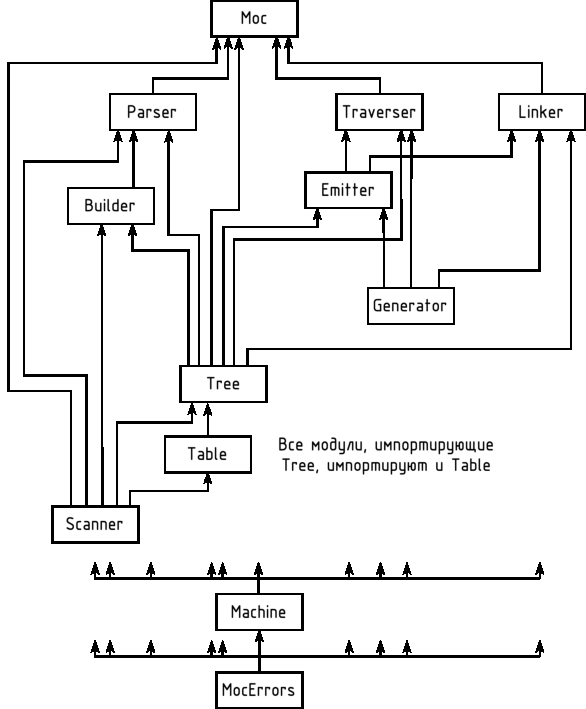
\includegraphics[width=\textwidth,keepaspectratio]{figures/modules.pdf}
\vspace{3mm}
\caption{Граф импорта модулей (стрелка от A к B означает, что модуль B импортирует модуль A).}
\label{fig:ModuleGraph}
\end{figure}

\begin{figure}[H]
\centering
\vspace{15mm}
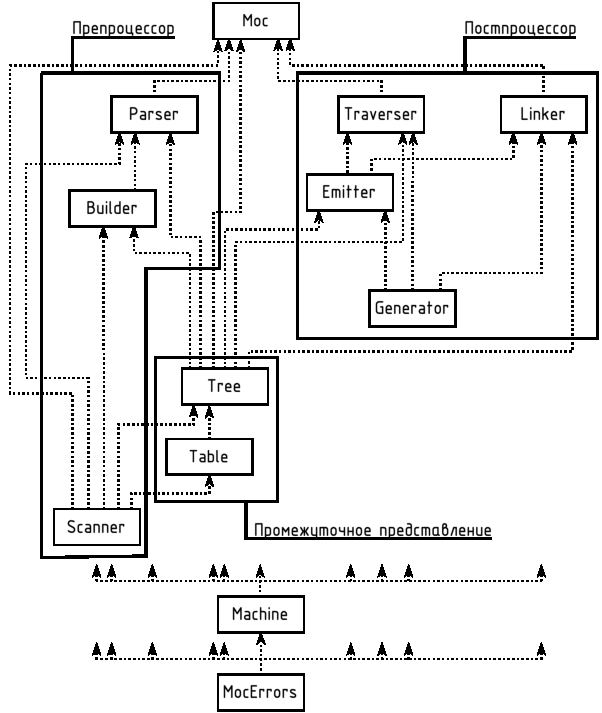
\includegraphics[width=\textwidth,keepaspectratio]{figures/modules2.pdf}
\vspace{3mm}
\caption{Схема разделения модулей на логические группы: препроцессор, постпроцессор и промежуточное представление.}
\label{fig:ModuleGraph2}
\end{figure}

\section{Загрузка текста}

\firstparskip Для начала процесса компиляции необходим предмет компиляции, то есть исходный код на языке программирования высокого уровня. Как правило, он находится в одном или нескольких файлах.

Сначала текст программы необходимо считать из файла и загрузить в оперативную память. Это может быть выполнено как целиком, так и по частям\tire по мере анализа. Язык Оберон спроектирован таким образом, чтобы обеспечивать возможность однопроходной компиляции: в частности, каждый программный объект должен быть объявлен до его использования.

Это правило имеет одно важное исключение, унаследованное ещё от языка Паскаль: при объявлении \textit{указательного} типа допустимо использовать в качестве базового такой тип, который на момент этого объявления ещё не определён. Такое исколючение представляется технически возможным благодаря тому, что на уровне машинной реализации все указатели представляют собой целочисленные значения одной и той же длины, а информация о типе, на который они ссылаются, интерпретируется лишь средствами языка высокого уровня. Другими словами, размер указателя не зависит от базового типа, что позволяет заранее определить структуру данных, содержащую ссылки на ещё не объявленные типы. Яркий пример использования этого исключения\tire объявление рекурсивных типов (см. листинг~\ref{lst:UndefinedPointerBase}).

\vspace{\baselineskip}
\captionsetup{type=listing}
\captionlisting{Рекурсивное объявление типов с использованием указателей}
\label{lst:UndefinedPointerBase}
\begin{modula2long}
TYPE
  Node = POINTER TO NodeDesc;     (* Здесь о типе NodeDesc ещё
                                         ничего не известно *)
  NodeDesc = RECORD
    data: INTEGER;
    next: Node     (* Типы Node и NodeDesc взаимно рекурсивны *)
  END;
\end{modula2long}

\needspace{5\baselineskip}
\subsection{Программный модуль как единица компиляции}

\firstparskip Теоретически важно определить \textit{единицу компиляции}, то есть законченный блок, который достаточен для того, чтобы выполнить его перевод в машинный код. Например, произвольную процедуру нельзя скомпилировать в отрыве от её контекста, потому что в ней, например, может быть обращение к глобальным переменным. Для компиляции необходимо знать их тип. Единицей компиляции в языке Оберон является модуль. Модуль, а не программа, является и единицей загрузки в операционных системах, построенных на базе Оберона (то есть пользователь ОС может загружать и выгружать каждый модуль отдельно от остальных). Наконец, модуль является синтаксическим началом языка Оберон, то есть целевым (или начальным) символом его грамматики~\cite[с.~235]{Sverdlov}\cite[с.~15]{Moldovanova}.

\subsection{Модуль Machine}

В данном компиляторе считывание текста из файла и отдача его в лексический анализатор осуществляется в модуле \code{Machine}\tire модуле, обеспечивающем связь компилятора с вычислительной платформой на которой он запущен. При переносе компилятора на другую платформу или при адаптации его к новому формату файла и т.~д. достаточно будет подправить модуль \code{Machine}. Остальные модули компилятора могут переноситься на новые платформы совершенно без изменений.

Модуль \code{Machine} определяет записной тип \code{Pos} (позиция) с полями \code{line} и \code{col}, означающими номер строки и номер столбца в файле. Предполагается, что файл сохранён в кодировке ASCII или UTF-8. Значение поля \code{col} хранит не количество \textit{байтов} от начала строки, а корректно подсчитывает литеры, что актуально в случае UTF-8.

Модуль экспортирует две переменные типа \code{Pos}: переменная \code{pos}\tire хранит текущую позицию в файле, а переменная \code{errorPos}\tire позицию последней возникшей ошибки. 

В модуле \code{Machine} также определены константы, характеризующие вычислительную платформу, такие как максимальное значение целочисленного типа, ширина экспоненты вещественного числа с плавающей запятой и ширина указательного типа.

\section{Лексический анализатор}

\firstparskip В каждом языке есть алфавит\tire набор элементарных знаков, из которых формируются слова и предложения. Программы записываются, в общем-то, теми же самыми буквами, цифрами и другими литерами, которыми мы пользуемся на письме в естественных языках. Несмотря на это, в случае языков программирования алфавит состоит не из букв, а из \textit{символов} (лексем).

Символы языка неделимы и также произвольно могут быть заменены на другие. Например, \code{BEGIN} и «\,\code{+}\,»\tire символы языка Оберон\tire могли бы быть заменены на \code{НАЧАЛО} и \code{ПЛЮС}, от этого в языке больше ничего бы не поменялось. Вообще набор символов языка программирования конечен, хотя некоторые из них, такие как числа и идентификаторы, представляют целые классы цепочек литер\tire теоретически бесконечные по вариантам своих значений. Например, оба символа \code{paramCount} и \code{x} являются идентификаторами, хотя и различными, а каждый из символов \code{4.6}, \code{0.0} и \code{276.08} представляет собой (с точностью до значения) не что иное как вещественное число. Следовательно, некоторые типы символов связаны с дополнительными данными. Таких «многоликих» символов в языке Оберон несколько, они перечислены в таблице \ref{tab:OberonSymbols}.

\vspace{5mm}
\begin{table}[H]
\centering
\caption{Символы языка Оберон, с которыми связаны дополнительные данные}
\label{tab:OberonSymbols}
\vspace{8pt}
\small
\begin{tabular}{@{} l l l @{}}
\toprule
  \parbox{2.7cm}{\vspace{1mm}\centering\noindent Наименование \\ символа\vspace{1mm}} & Пример & Дополнительные данные \\
\midrule
  \code{ident}  & \code{Out}     & строка (цепь литер) \\
  \code{int}    & \code{217}     & число типа \code{INTEGER} \\
  \code{real}   & \code{15.53}   & число типа \code{REAL} \\
  \code{string} & \code{"Hello"} & строка (цепь литер) и её длина \\
  \code{char}   & \code{61X}     & литера \\
\bottomrule
\end{tabular}
\end{table}

На этапе лексического анализа входной поток литер разбивается (или соединяется) на символы, то есть лексические единицы языка, часто состоящие из многих литер. Лексический анализ ничего не знает о грамматике языка. Всё, что он умеет,\tire разбивать линейный поток литер на линейный поток символов, попутно отбрасывая пробелы, знаки табуляции, переносы строк и комментарии.

В языке Оберон комментарии могут быть вложенными, поэтому лексический анализ учитывает и этот аспект. При этом в Обероне нет «однострочных» комментариев, которые бы работали до конца строки. Единственный вид комментария в Обероне\tire текст, заключённый в скобки со звёздочками: \code{(*}~\ldots~\code{*)}. Такой формат комментариев был ещё в Паскале, наряду с фигурными скобками \code{\{}~\ldots~\code{\}}. В~языке Оберон фигурные скобки используются для указания литералов типа множество\footnote{Речь о литералах типа \code{SET}, см. с.~\pageref{OberonSets} настоящей работы.}.

Если пробелы встречаются внутри строкового литерала (то есть заключены в кавычки), они не отбрасываются анализатором\tire содержимое строки воспринимается буквально и передаётся на следующий этап разбора без изменений. Более того, Оберон не определяет никаких специальных последовательностей внутри строковых литералов. Например, последовательность входных литер «\,\code{"\textbackslash t\textbackslash n"}\,» будет распознана компилятором как строковой литерал, состоящий из 4 литер: «\code{\textbackslash}», «\code{t}», «\code{\textbackslash}» и «\code{n}».

Лексический анализатор выполнен в виде модуля \code{Scanner}. Модуль определяет 66 целочисленных констант, каждая из которых означает некоторый символ, выдаваемый анализатором (см. листинг~\ref{lst:SymbolConstants}). Символ \code{null} не экспортирован, потому что он используется только внутри самого модуля анализатора для пропуска комментариев и определения ошибочных входных литер.

\begin{listing}[H]
\caption{Полный список лексических символов языка Оберон}
\vspace{-17pt}
\label{lst:SymbolConstants}
\begin{modula2}
CONST
  (** Лексические символы **)
  null        =  0;    times*     = 1;      rdiv*      = 2;
  div*        =  3;    mod*      = 4;      and*      = 5;
  plus*       =  6;    minus*    = 7;      or*        = 8;
  eql*        =  9;    neq*      = 10;     lss*       = 11;
  leq*        = 12;    gtr*       = 13;     geq*      = 14;
  in*         = 15;     is*        = 16;     arrow*   = 17;
  period*     = 18;    char*      = 20;    int*       = 21;
  real*       = 22;    false*     = 23;    true*     = 24;
  nil*         = 25;    string*    = 26;    not*      = 27;
  lparen*     = 28;    lbrak*     = 29;    lbrace*   = 30;
  ident*      = 31;     if*        = 32;    while*     = 34;
  repeat*    = 35;    case*      = 36;    for*       = 37;
  comma*    = 40;    colon*      = 41;    becomes* = 42;
  upto*      = 43;    rparen*    = 44;    rbrak*    = 45;
  rbrace*    = 46;    then*      = 47;    of*        = 48;
  do*        = 49;    to*         = 50;    by*       = 51;
  semicolon* = 52;    end*        = 53;    bar*      = 54;
  else*      = 55;    elsif*       = 56;    until*     = 57;
  return*    = 58;    array*      = 60;    record*   = 61;
  pointer*   = 62;    const*      = 63;    type*     = 64;
  var*       = 65;    procedure*  = 66;    begin*    = 67;
  import*    = 68;    module*     = 69;    eot*      = 70;
\end{modula2}
\end{listing}

Кроме того, определены константы $\code{identSize} = 256$ и $\code{stringSize} = 1024$. Это максимальная длина идентификатора и максимальная длина строкового литерала. При превышении длин в исходном коде лексический анализатор выдаёт ошибку. После этого разбор продолжается. Это сделано для того, чтобы компилятор выдавал программисту целый список ошибок, а не останавливался на первой. Такой же подход использован и в синтаксическом анализаторе. В~\cite{WirthCompiler} Вирт указывает, что продолжение разбора входного текста после ошибок\tire важная черта компилятора, необходимое условие удобства его эксплуатации. Но, вместе с тем, это непростая задача, требующая творческого подхода, потому что по сути компилятор в некотором смысле должен корректно проанализировать \textit{некорректно} написанную программу\tire про которую точно известно, что в ней есть ошибка. Недетерминированный и неформализованный характер данной задачи обуславливает сложность её решения.

Определены и типы данных \label{ScannerIdentType}\code{Ident} и \code{StrVal}\tire массивы литер, длиной \code{identSize} и \code{stringSize}.

Основная процедура, экспортированная данным модулем,\tire процедура \code{Get}. Многократный её вызов из другого модуля\tire модуля \code{Parser}\tire и осуществляет собственно лексический разбор текста.

Модуль \code{Scanner} также определяет несколько экспортированных переменных, доступных только для чтения, и одну неэкспортированную переменную \code{ch}.

\begin{listing}[H]
\caption{Глобальные переменные модуля Scanner}
\vspace{-17pt}
\begin{modula2}
VAR
  (** Results of Get **)
  name*: Ident;
  intVal*: INTEGER;
  realVal*: REAL;
  strVal*: StrVal;
  strLen*: INTEGER;

  (** - **)
  ch: CHAR; (** Read-ahead character *)
\end{modula2}
\end{listing}

Глобальная переменная \code{ch} литерного типа используется для реализации метода лексического анализа с заглядыванием вперёд на одну литеру (look ahead). Смысл этого метода в том, что он решает следующую проблему. При считывании из файла одной литеры за другой в общем случае невозможно определить, будет ли следующая литера относиться к текущему лексическому символу или нет. Например, начав работу и считав литеру «$4$» (ASCII-код $52$), лексический анализатор может прийти к выводу, что перед ним начало числа. Считав следующую литеру, например «$7$», начало числа выглядит уже как «$47$».

Но стоит ли читать дальше? Если будет считана очередная цифра (скажем, «$3$»), она будет приписана к числу:
$$x' = 10x +(\mathit{ch}-48),$$
\noindent где $x$\tire старое значение числа ($47$), $\mathit{ch}$\tire ASCII-код считанной литеры, т.~е. цифры «$3$» (ASCII-код $51$), а 48\tire ASCII-код цифры нуль.

Если вместо литеры «$3$» будет считан пробел, то его можно просто отбросить. При следующем вызове разбор начнётся с новой литеры, а пробел при разборе всё равно пропускается.

Но если следующая литера после «$47$» будет «\,\code{<}\,», то перед нами проблема. Просто так отбросить эту литеру нельзя, ведь это часть лексического символа, который должен быть выдан \textit{при~следующем} запуске процедуры \code{Get}. Ситуация осложняется ещё и тем, что литера «\,\code{<}\,» может оказаться как самостоятельным символом\tire знаком меньше ($\code{lss} = 11$), так и первой литерой символа «меньше или равно» («\,\code{<=}\,», $\code{leq} = 12$).

Метод чтения с заглядыванием на одну литеру вперёд решает эту проблему\tire при любом запуске процедуры \code{Get} разбор начинается с литеры, находящейся в глобальной переменной \code{ch}\tire к этому моменту в ней уже находится заранее считанная из файла литера. По окончании работы процедуры, она обязана обеспечить, чтобы в той же глобальной переменной находилась литера, непосредственно следующая за последней из тех, которые были отнесены к текущему лексическому символу. Разумеется, это требование в силе только в том случае, если такая литеры вообще есть. Если достигнут конец файла, в \code{ch} должна быть помещена литра с кодом 0\tire т.~е. значение~\code{0X}\footnote{Буква «X» в конце шестнадцатеричного числа на языке Оберон означает, что данное число\tire литерал типа \codef{CHAR}. Например, \codef{0AX}\tire литера с ASCII-кодом 10, «перевод строки».}.

\section{Нисходящий рекурсивный синтаксический анализатор}

\firstparskip За этапом лексического разбора следует разбор синтаксический. Входными данными для данного этапа разбора выступают лексические символы. Задача синтаксического разбора\tire распознать в них (многократно вложенные друг в друга) конструкции языка. Задача синтаксического разбора сильно упрощена за счёт того, что лексический анализатор выделен в отдельный модуль и на данном этапе совершенно не надо заботиться о пробелах, комментариях, правильном составе идентификаторов и любых других нюансов лексики.

Синтаксический анализатор выполнен в виде модуля \code{Parser}. Входные символы на этом этапе\tire неделимые единицы, возможно, несущие дополнительную информацию. Перед началом разбора синтаксический анализатор обращается к лексическому анализатору за первым символом и помещает его в глобальную переменную \code{sym} (в модуле \code{Parser}). Происходит это посредством вызова \code{Scanner.Get(sym)}. Процедуры анализатора будут в первую очередь обращаться за «следующим» входным символом к этой переменной. Если символ действительно относится к данной процедуре, то после его обработки снова будет вызвана процедура \code{Scanner.Get}. Таким образом, обеспечивается работа анализатора с заглядыванием вперёд на один \textit{символ}. Это похоже на соответствующий приём в модуле \code{Scanner}, где было реализовано заглядывание на одну \textit{литеру} вперёд.

Кроме (нэкспортированной) глобальной переменной \code{sym} модуль \code{Parser} определяет переменную \code{modName} типа \code{Ident}\footnote{См. с.~\pageref{ScannerIdentType} настоящей работы.}, которая содержит имя разбираемого в данный момент модуля. \code{modName} принимает своё значение при разборе начального нетерминала \code{Module}, а в конце разбора этого нетерминала значение сверяется с именем после \code{END}\footnote{В Обероне название модуля и процедуры пишется повторно после закрывающего соответствующую конструкцию слова \codef{END}.}.

Наиболее подходит для Оберона синтаксический разбор методом рекурсивного спуска. Идея этого метода в том, что для каждого нетерминала, выраженного в РБНФ, (иными словами, для каждой конструкции языка) пишется отдельная распознающая процедура. В~ходе разбора соответствующей конструкции процедура считывает из входного потока все символы, производимые данным нетерминалом. Если правила для данного нетерминала содержат в правых частях другие нетерминалы, процедура вызывает соответствующие распознающие процедуры. Данный метод подробно разобран в \cite{WirthCompiler,Sverdlov}.

Важно, чтобы после разбора соответствующей конструкции распознающая процедура оставляла в глобальной переменной \code{sym} символ, следующий сразу за концом данной конструкции.

Рассмотрим часть синтаксиса Оберона, связанную с начальным нетерминалом \code{modulis} (см. листинг~\ref{lst:Syntax:Module}). Полный синтаксис Оберона в формате РБНФ есть в приложении~\ref{appendix:OberonSyntax}.

\begin{listing}[H]
\caption{Модуль\tire начальный нетерминал в РБНФ}
\vspace{-17pt}
\label{lst:Syntax:Module}
\begin{ebnf}
модуль = MODULE ident ";" [СписокИмпорта]
         ПоследовательностьОбъявлений
         [BEGIN ПоследовательностьОператоров]
         END идентификатор ".".

идентификатор = буква {буква | цифра}.
СписокИмпорта = IMPORT импорт {"," импорт} ";".
импорт = [идентификатор ":="] идентификатор.

ПоследовательностьОбъявлений =
        [CONST {ОбъявлениеКонстанты ";"}]
        [TYPE {ОбъявлениеТипа ";"}]
        [VAR {ОбъявлениеПеременных ";"}]
        {ОбъявлениеПроцедуры ";"}.

ПоследовательностьОператоров = оператор {";" оператор}.
\end{ebnf}
\end{listing}

В соответствии с этим фрагментом определения на РБНФ в модуле \code{Parser} определены процедуры \code{Module}, \code{Import}, \code{DeclarationSequence}, \code{ConstDeclaration}, \code{TypeDeclaration}, \code{VariableDeclaration}, \code{ProcedureDeclaration}, \code{Statement} и \code{StatementSequence}.

Аналогично оформлены и другие нетерминалы. Но это соответствие между нетерминалами РБНФ и процедурами не абсолютное: например, нетерминал \code{ImportaSaraksts} не находит выражения в отдельной процедуре\tire его код встроен прямо в процедуру \code{Module}. Это не приводит к дублированию кода или другим проблемам, поскольку нетерминал \code{ImportaSaraksts} используется только в правой стороне определения нетерминала \code{Module}, т.~е. он вообще выделен в отдельный нетерминал для удобства или наглядности определения. По соображениям же программирования бывает лучше снова соединить эти процедуры в одну.

Распознавающая процедура, соответствующая нетерминалу \code{modulis}, показана в листинге~\ref{lst:Parser:Module}. Это функциональная процедура, тип возвращаемого ею значения\tire \code{Tree.Node}\tire будет подробно рассмотрен в гл.~\ref{sec:IntermediateRepresentation} (с.~\pageref{ModuleTree}). При разбиении компилятора на препроцессор и постпроцессор, процедуры синтаксического анализа не запускают процедуры генератора машинного кода напрямую, а создают и возвращают узлы дерева. Эту узлы собираются в единое абстрактное синтаксическое дерево, которое и является результатом работы препроцессора и\tire процедуры \code{Module}.

\captionsetup{type=listing}
\captionlisting{Процедура распознавания начального нетерминала}
\label{lst:Parser:Module}
\begin{modula2long}
(** module = MODULE ident ";" [ImportList]
    DeclarationSequence [BEGIN StatementSequence]
    END ident ".".
    ImportList = IMPORT import {"," import} ";". *)
PROCEDURE Module(): Tree.Node;
VAR module: Tree.Node;
  name: Ident;
  procedures, statementSequence: Tree.Node;
BEGIN
  Skip(S.module);
  IF Check(S.ident) THEN
    Strings.Copy(S.name, modName);
    S.Get(sym); (* ident *)

    (* IMPORT *)
    Skip(S.semicolon);
    IF Skipped(S.import) THEN
      Import;
      WHILE Skipped(S.comma) DO
        Import
      END;
      Skip(S.semicolon)
    END;

    (* CONST, TYPE, VAR and BEGIN *)
    procedures := DeclarationSequence();
    IF Skipped(S.begin) THEN
      statementSequence := StatementSequence()
    END;

    module := Builder.Enter(procedures, statementSequence, NIL);
    Skip(S.end);
    IF Check(S.ident) THEN
      IF S.name # modName THEN
        Machine.Error(Errors.modNameMismatch)
      ELSE
        S.Get(sym); (* ident *)
        Skip(S.period)
      END
    END
  END
RETURN module END Module;
\end{modula2long}

Узел дерева, соответствующий конструкции \code{module}, имеет класс \code{NEnter}. Для его создания используется процедура \code{Enter} модуля-построитель дерева \code{Builder}. Она и создаёт узел соответствующего класса. В~нижнем поддереве этого узла будут находиться процедуры модуля, а в правом поддереве\tire последовательность операторов, выполняемая при инициализации модуля (операторы, находящиеся после главного \code{BEGIN}).

Вспомогательные процедуры \code{Skip}, \code{Skipped} и \code{Check} используются вместо операторов \code{IF} для более удобной записи алгоритма (см. листинг~\ref{lst:SkipSkippedCheck}).

\captionsetup{type=listing}
\captionlisting{Вспомогательные процедуры синтаксического анализатора}
\label{lst:SkipSkippedCheck}
\begin{modula2long}
(** Reports whether sym is the expected symbol.
    If not, reports an error. *)
PROCEDURE Check(expectedSym: INTEGER): BOOLEAN;
BEGIN
  IF sym # expectedSym THEN
    Machine.ErrorExpected(expectedSym, sym)
  END
RETURN sym = expectedSym END Check;

(** Checks that sym is the expected symbol
    and skips it, or reports an error. *)
PROCEDURE Skip(expectedSym: INTEGER);
BEGIN
  IF sym = expectedSym THEN
    S.Get(sym)
  ELSE
    Machine.ErrorExpected(expectedSym, sym)
  END
END Skip;

(** If sym is the expected symbol then skips it and
    returns true, otherwise returns false. *)
PROCEDURE Skipped(expectedSym: INTEGER): BOOLEAN;
VAR ok: BOOLEAN;
BEGIN
  ok := sym = expectedSym;
  IF ok THEN S.Get(sym) END
RETURN ok END Skipped;
\end{modula2long}

Процедура \code{Check} проверяет, является ли текущий символ переданным ей в качестве параметра. В~случае несовпадения выдаётся ошибка компиляции вида «\textit{This expected, but that found}», где «\textit{this}» и «\textit{that}» заменяются конкретными названиями символов. Это происходит в модуле \code{Machine}. Если же символ совпал, он остаётся на месте для дальнейшего анализа\tire это полезно, если это, например, символ \code{int}, \code{real} или \code{string}.

Процедура \code{Skip} работает аналогично процедуре \code{Check}, но пропускает символ в случае совпадения.

Процедура \code{Skipped} используется несколько иначе. Она не выдаёт ошибки, но пропускает символ в случае совпадения. Это удобно в тех случаях в ходе разбора конструкции, когда присутствие символа необязательно, но от этого зависит дальнейший разбор. Например, после прочтения обязательных символов \code{module}, \code{ident} и \code{semicolon}, соответствующих ключевому слову \code{MODULE}, имени модуля и точки с запятой, может следовать ключевое слово \code{IMPORT}, но его присутствие в коде программы необязательно. В~этом месте при разборе используется конструкция \code{IF Skipped(S.import) THEN}.

\needspace{5\baselineskip}
Процедура \code{ErrorExpected} в модуле \code{Machine}, выдающая сообщение об ошибке несоответствия символа, приведена в листинге~\ref{lst:ErrorExpected}.

\captionsetup{type=listing}
\captionlisting{Процедура вывода ошибки несоответствия символа}
\label{lst:ErrorExpected}
\begin{modula2long}
PROCEDURE ErrorExpected*(symExpected, symFound: INTEGER);
BEGIN
  IF BeginError() THEN
    Errors.PrintSymbol(symExpected);
    Out.String(' expected, but ');
    Errors.PrintSymbol(symFound);
    Out.String(' found');
    Out.Ln
  END
END ErrorExpected;
\end{modula2long}

Для вывода конкретных наименований символов используется модуль \code{Errors}, который умеет переводить числа, соответствующие символам, в их строковое выражение.

\needspace{15\baselineskip}
Процедура \code{StatementSequence}, распознающая последовательность операторов, выглядит следующим образом:

\begin{listing}[H]
\caption{Распознающая процедура последовательности операторов}
\vspace{-17pt}
\begin{modula2}
(** StatementSequence = statement {";" statement}. *)
PROCEDURE StatementSequence(): Tree.Node;
VAR first, prev, statement: Tree.Node;
BEGIN
  (* Sync *)
  IF ¬((sym >= S.ident) & (sym <= S.for) OR
       (sym >= S.semicolon))
  THEN
    Machine.Error(Errors.noStatement);
    REPEAT S.Get(sym) UNTIL (sym >= S.ident)
  END;

  WHILE sym = S.semicolon DO S.Get(sym) END;
  first := Statement();
  prev := first;
  WHILE Skipped(S.semicolon) DO
    WHILE sym = S.semicolon DO S.Get(sym) END;
    statement := Statement();
    prev.link := statement;
    prev := statement
  END
RETURN first END StatementSequence;
\end{modula2}
\end{listing}

\needspace{15\baselineskip}
Непосредственно связанная с ней процедура \code{Statement}, распознающая единичный оператор, имеет следующий вид:

\begin{listing}[H]
\caption{Распознающая процедура для оператора}
\vspace{-17pt}
\label{lst:Parser:Statement}
\begin{modula2}
(** statement = [assignment |\textbar| ProcedureCall |\textbar| IfStatement |\textbar|
    CaseStatement |\textbar| WhileStatement |\textbar| RepeatStatement |\textbar|
    ForStatement]. *)
PROCEDURE Statement(): Tree.Node;
VAR statement, designator: Tree.Node;
BEGIN
  IF sym = S.ident THEN (* Assignment or procedure call *)
    designator := Designator();
    IF Skipped(S.becomes) THEN
      statement := Assignment(designator)
    ELSE
      statement := ProcedureCall(designator)
    END
  ELSIF Skipped(S.if) THEN
    statement := IfStatement()
  ELSIF Skipped(S.while) THEN
    statement := WhileStatement()
  ELSIF
    (* ... *)
  END
RETURN statement END Statement;
\end{modula2}
\end{listing}

Аналогично процедурам \code{Module}, \code{StatementSequence} и \code{Statement} выполнены и другие распознающие процедуры.

В Обероне четыре уровня приоритетов операций: \textit{выражение} (expression), \textit{простое выражение} (simple expression), \textit{слагаемое} (term) и \textit{множитель} (factor). Как определение этих нетерминалов в РБНФ, так и соответствующие им процедуры являются рекурсивными. Выражение состоит из одного или двух простых выражений. Простое выражение состоит из одного или более слагаемых. Слагаемое состоит из одного или более множителей.

Наконец, множитель может представлять собой массу различных конструкций, как простых, так и сложных: число, строковой литерал, \code{NIL}, \code{TRUE}, \code{FALSE}, конструкцию отрицания, литерал-множество, идентификатор (возможно, с прикреплённым к нему одним или несколькими указаниями индекса массива или поля записи). Кроме всего прочего, множитель может представлять собой \textit{выражение} в скобках. Таким образом организована косвенная рекурсия из четырёх процедур. Но рекурсия может замкнуться и по другому маршруту: например, при указании индекса в массиве также используется \textit{выражение}.

Возьмём для примера элементарное выражение «$75$». Примем, для определённости, что следующий за этим числом символ\tire точка с запятой (класс \code{semicolon}). Данное выражение элементарное, поскольку оно сводится к одному единственному лексическому символу\tire целому числу $75$. Но, чтобы это узнать, синтаксический анализатор проделывает следующий путь: сначала запускается процедура \code{Expression}, она вызывает \code{SimpleExpression} (в исходном коде видно, что такой вызов\tire первое действие, которое она осуществляет). В~свою очередь, \code{SimpleExpression} вызывает процедуру \code{Term}\footnote{Перед вызовом \codef{Term} процедура \codef{SimpleExpression}, в соответствии с определением соответствующего нетерминала в РБНФ, успевает проверить, нет ли перед ней знака минус или знака плюс. В~нашем примере $\mathit{sym} = \mathit{int}$ и $\mathit{intVal} = 75$.}, а та\tire процедуру \code{Factor}.

Процедура \code{Factor} заходит в ветвь \code{IF}, которая соответствует условию $\mathit{sym} = int$ и с помощью процедуры \code{NewIntConst}, экспортированной модулем \code{Builder}, создаёт узел-константу с классом \code{NConst}, возвращает этот узел и завершается. Таким образом, из \code{Factor} мы попадаем обратно в \code{Term}.

Процедура \code{Term} переходит к вычислению условия оператора \code{WHILE}\footnote{Условие $(\mathit{times} \leqslant \mathit{sym} \leqslant \mathit{and})$ эквивалентно условию $(\mathit{sym} = \mathit{times}) \vee (\mathit{sym} = \mathit{rdiv}) \vee (\mathit{sym} = \mathit{div}) \vee (\mathit{sym} = \mathit{mod}) \vee (\mathit{sym} = \mathit{and})$, то есть в широком смысле всем возможным операциям умножения и деления.}.

\begin{align}
& (\mathit{times} \leqslant \mathit{sym} \leqslant \mathit{and})
\end{align}

Это условие оказывается ложным, поэтому процедура завершается, возвращая в качестве результата узел, полученный из \code{Factor}. И~из \code{Term} мы возвращаемся в \code{SimpleExpression}.

Процедура \code{SimpleExpression} после вызова \code{Term} также переходит к циклу \code{WHILE}\footnote{Условие $(\mathit{plus} \leqslant \mathit{sym} \leqslant \mathit{or})$ эквивалентно условию $(\mathit{sym} = \mathit{plus}) \vee (\mathit{sym} = \mathit{minus}) \vee (\mathit{sym} = \mathit{or})$, то есть в широком смысле всем возможным операциям сложения и вычитания.} с похожим условием.

\begin{align}
& (\mathit{plus} \leqslant \mathit{sym} \leqslant \mathit{or})
\end{align}

И это условие оказывается ложным,\tire и узел, созданный ещё в \code{Factor}, передаётся теперь в качестве результата вызова \code{SimpleExpression} в процедуру \code{Expression}.

Процедура \code{Expression} теперь должна определить, нужно ли вызывать второй \code{SimpleExpression} справа от знака сравнения, т.~е. есть ли этот знак в исходном коде. Поэтому она подряд проверяет три условия, соответствующие трём ветвям оператора \code{IF}\footnote{Условие $(\mathit{eql} \leqslant \mathit{sym} \leqslant \mathit{geq})$ эквивалентно условию $(\mathit{sym} = \mathit{eql}) \vee (\mathit{sym} = \mathit{neq}) \vee (\mathit{sym} = \mathit{lss}) \vee (\mathit{sym} = \mathit{leq}) \vee (\mathit{sym} = \mathit{gtr}) \vee (\mathit{sym} = \mathit{geq})$, т. е. всем возможным операциям сравнения.}:

\begin{align}
& (\mathit{eql} \leqslant \mathit{sym} \leqslant \mathit{geq}) \\
& (\mathit{sym} = \mathit{in}) \\
& (\mathit{sym} = \mathit{is})
\end{align}

Все три условия оказываются ложными, и поэтому процедура \code{Expression} завершается.

\subsection{Модуль Builder}

Важно отметить, что уже на этапе препроцессора должны выполняться некоторые простейшие оптимизации. Дело в том, что при объявлении констант их значение должно быть константным \textit{выражением}, то есть оно не обязательно должно быть литералом того или иного типа\tire оно может быть и более сложным выражением. Но требуется, чтобы все его составные звенья также были константными (см. листинг \ref{lst:ConstExpressions}), и, как следствие, чтобы значение такой константы могло быть вычислено в момент компиляции, а не только в момент исполнения программы. То же самое касается и задания длины массива.

\begin{listing}[H]
\caption{Пример использования константных выражений}
\vspace{-17pt}
\label{lst:ConstExpressions}
\begin{modula2}
CONST
  x = 25;
  y = (x + x) MOD 20;
  z = x * y + x DIV y;

TYPE Array = ARRAY z * 4 DIV 5 + 3 OF INTEGER;
\end{modula2}
\end{listing}

Для этого построитель \code{Builder}, когда ему дают команду создать новый узел\tire операцию «\,\code{+}\,»\tire не спешит сразу создавать его. Сначала он проверяет, не являются ли оба операнда константами (узлами класса \code{NConst}). Если это так, то вместо создания третьего узла и объединения двух поддеревьев модуль построитель возвращает один константный узел, значение которого уже на этом этапе оказывается полностью вычисленным.

\section{Проверка типов}

\firstparskip Оберон\tire язык со строгой типизацией, поэтому компилятор в ходе своей работы должен обеспечивать согласование типов при присваивании, а также при передаче параметров в процедуры.

Если брать только синтаксис языка Оберон, а значит не учитывать контекстную информацию, в частности типы данных, то выражение «\,\code{25 DIV TRUE + "R" - ORD(48)}\,» окажется вполне корректным. Однако оно полностью лишено смысла. Отсюда можно сделать вывод, что синтаксис языка не касается согласования типов.

Проверку типов удобно осуществлять в синтаксическом анализаторе, так как, во-первых, она не сильно усложняет его, а во-вторых, синтаксическому анализатору время от времени нужны знания о типах данных, с которыми он работает. Дело в том, что охрана типа (type guard) в Обероне синтаксически совпадает с вызовом процедуры: и в том, и в другом случае за идентификатором следует открывающая круглая скобка. Если в данном контексте идентификатор обозначает процедуру, то перед нами процедурный вызов. В~противном случае компилятор воспримет это место как охрану типа. Поэтому учёт контекста важно производить уже на этапе синтаксического разбора.

Для проверки корректности типизации в выражениях, подобных $x = y$, синтаксическому анализатору требуется информация о типах \textit{простых выражений} $x$ и~$y$, поскольку необходимо исключить случаи несогласованных сравнений, например, между числом и строкой.

Данный компилятор разделён на препроцессор и постпроцессор, между которыми лежит граница в виде промежуточного представления\tire абстрактного синтаксического дерева. Поэтому к моменту, когда разбор достигает операции сравнения, выражения $x$ и $y$ уже представлены в виде готовых поддеревьев. К~счастью, корневая вершина каждого из них содержит информацию о типе соответствующего простого выражения.

Следует отметить, что каждое из таких поддеревьев\tire будь то $x$ или $y$\tire может представлять собой как простой терминальный узел класса \code{NConst} с числовой константой, так и весьма разветвлённое дерево, включающее вызовы функциональных процедур, разыменование указателей, переход к элементам массивов и прочее. В~любом случае, информация о типе данных сохраняется, в том числе, в корне поддерева, что значительно упрощает синтаксический разбор: нет необходимости повторно углубляться в уже построенные поддеревья.

Если в компиляторе отсутствует явное разделение на препроцессор и постпроцессор и машинный код генерируется непосредственно в процессе синтаксического разбора\tire как это реализовано, например, в компиляторе Вирта~\cite{WirthCompiler} и компиляторе Интер-Оберон~\cite{InterOberon,InterOberonVideo},\tire то синтаксический анализатор вместо узлов типа \code{Tree.Node} оперирует так называемыми предметами\tire записями типа \code{Item}, которые переносят ту же самую информацию, которую несут вершины деревьев в нашем случае. С~точки зрения программной реализации распознающие процедуры тогда передают результат не через \code{RETURN}, а через параметры-переменные. Это позволяет вовсе не использовать динамическую память при синтаксическом разборе\footnote{\ldots если не считать размещаемой в динамической памяти таблицы символов. См. с.~\pageref{sec:SymbolTable} настоящей работы.}.

\section{Промежуточное представление программы}
\label{sec:IntermediateRepresentation}

\firstparskip Два модуля\tire \code{Tree} и \code{Table}\tire составляют границу между препроцессором и постпроцессором. Обычно в компиляторах Оберона эту роль выполняет один модуль. Мы же решили разделить его на два, поскольку эти модули решают различные обособленные задачи.

\subsection{Таблица символов}

\label{sec:SymbolTable}

Модуль \code{Table} имеет такое название, поскольку исторически сложилось, что данные об объявлениях называются в компиляторах «таблицей символов». На самом деле они мало напоминают таблицу\tire скорее, это граф.

В~ходе синтаксического разбора препроцессор заполняет модуль \code{Table} данными об импортированных при компиляции модулях, объявленных константах, типах данных и глобальных переменных. Все эти данные хранятся непосредственно в модуле \code{Table} в виде динамической структуры данных и извлекаются из неё постпроцессором в ходе обхода абстрактного синтаксического дерева.

Всё содержимое таблицы символов модуль \code{Table} удерживает за один указатель\tire \code{topScope}. Тип этого указателя\tire \code{Object}, а базовый его тип\tire \code{ObjectDesc}\footnote{Вообще, сокращение «Desc» означает «descriptor» (описатель).}. Кроме этого, модуль \code{Table} определяет типы \code{ConstVal}, \code{Type} и \code{Module} (см. листинг~\ref{lst:TableTypes}). Последний является расширением типа \code{Object}.

\code{Object} всегда обозначает \textit{именованный} объект.

% Breakable captioned listing (not a float)
\captionsetup{type=listing}
\captionlisting{Структура данных модуля Table}
\label{lst:TableTypes}
\begin{modula2long}
TYPE
  Ident* = Scanner.Ident;
  StrVal* = Scanner.StrVal;

  ConstVal* = POINTER TO ConstValDesc;
  Type* = POINTER TO TypeDesc;
  Object* = POINTER TO ObjectDesc;
  Module* = POINTER TO ModuleDesc;

  ConstExt* = POINTER TO ConstExtDesc;
  ConstExtDesc*= RECORD
    s*: StrVal
  END;
    
  ConstValDesc* = RECORD
    ext*: ConstExt; (** Для строковых констант *)
    intVal*: INTEGER;
    realVal*: REAL;
    setVal*: SET
  END;
    
  TypeDesc* = RECORD 
    form*: INTEGER; (** См. константы Type.form *)
    paramCount*: INTEGER;
    len*: INTEGER;
    size*: INTEGER; (** В байтах *)
    base*: Type;
    dsc*: Object; (** Объект-потомок *)
    typeObj*: Object (** Оригинальный объект,
                         который ввёл тип *)
  END;

  ObjectDesc* = RECORD
    class*: INTEGER; (** См. константы Object.class *)
    name*: Ident;
    dsc*: Object; (** Объект-потомок *)
    type*: Type;
    constVal*: ConstVal;
    next*: Object
  END;

  ModuleDesc* = RECORD(ObjectDesc)
    originalName*: Ident (** Оригинальное имя модуля,
                             а name - это псевдоним *)
  END;
\end{modula2long}

Для каждого базового типа данных определена глобальная переменная (см. листинг~\ref{lst:BaseTypes}). Кроме переменной \code{topScope}, указывающей на вершину графа объектов, определённых в программе, есть ещё две переменные того же типа: \code{universe} и \code{system}. 

\begin{listing}[H]
\caption{Глобальные переменные модуля Table}
\vspace{-17pt}
\label{lst:BaseTypes}
\begin{modula2}
VAR topScope*, universe, system*: Object;
  byteType*, boolType*, charType*, intType*, realType*,
    setType*, nilType*, noType*, strType*: Type;
\end{modula2}
\end{listing}

Переменная \code{universe} указывает на начало области видимости, которая соответствует уровню, на котором находятся встроенные в язык объекты, такие как \code{INTEGER} или \code{BOOLEAN} (предобъявленные базовые типы данных), процедуры увеличения и уменьшения чисел \code{INC} и \code{DEC} или встроенные функции \code{ORD}, \code{CHR} и \code{LEN}.

Переменная \code{system} указывает на закрытую для обычного доступа область видимости. Это содержимое псевдомодуля \code{SYSTEM}: процедура \code{SIZE}, \code{ADR}, \code{PUT} и другие. Они становятся доступны только при обращении к модулю \code{SYSTEM} (разумеется, только после того, как его импортируют). В синтаксическом анализаторе псевдомодуль \code{SYSTEM} обрабатывается отдельной ветвью \code{IF}.

Все эти глобальные переменные получают своё изначальное значение при инициализации модуля \code{Table} (см. листинг~\ref{lst:TableInit}).

\captionsetup{type=listing}
\captionlisting{Инициализация модуля Table}
\label{lst:TableInit}
\begin{modula2long}
BEGIN
  byteType := NewType(Int,       1);
  boolType := NewType(Bool,     1);
  charType := NewType(Char,     1);
  intType   := NewType(Int,      4);
  realType := NewType(Real,     4);
  setType  := NewType(Set,      4);
  nilType   := NewType(NilType,  8);
  noType   := NewType(NoType,  4);
  strType  := NewType(String,    8);

  (* Инициализация объектов универсума *)
  (* Стандартные функции *)
  (* ... *)
  Enter('LEN', SFunc, intType,   1, lenFunc);
  Enter('CHR', SFunc, charType, 1, chrFunc);
  Enter('ORD', SFunc, intType,   1, ordFunc);

  (* Стандартные процедуры *)
  (* ... *)
  Enter('DEC', SProc, noType, 1, decProc);
  Enter('INC', SProc, noType, 1, incProc);

  (* Типы *)
  (* ... *)
  Enter('BOOLEAN', Typ, boolType, 0, 0);
  (* ... *)
  Enter('INTEGER',  Typ,  intType,  0, 0);

  OpenScope;
  topScope.next := system;
  universe := topScope;
  system := NIL;

  (* Инициализация небезопасных объектов
     псевдомодуля SYSTEM *)
  (* Функции *)
  Enter('SIZE', SFunc, intType, 1, sizeFunc);
  Enter('ADR', SFunc, intType, 1, adrFunc);
  (* ... *)
\end{modula2long}

Тип \code{Type} используется для сохранения информации о типах данных. Каждый базовый тип связан с соответствующим экземпляром \code{Type}. Например, глобальная переменная \code{intType} в модуле \code{Table} указывает на такой экземпляр. Когда в программе объявляется переменная, например \code{x} типа \code{INTEGER}, в области видимости \code{topScope} создаётся новый объект \code{x}. Его поле \code{name} заполняется значением \code{"x"}, класс принимает значение \code{Var}, а поле \code{type} начинает указывать туда же, куда указывает глобальная переменная \code{intType}.

У записей типа \code{Type} есть и обратный указатель на \code{Object}\tire это нужно для тех случаев, когда у типа есть псевдонимы. Оригинальное название типа содержится в поле \code{name} записи \code{Object}, на которую указывает поле \code{typeObj} записи типа \code{Type}.

\subsection{Абстрактное синтаксическое дерево}

\label{ModuleTree}

В отличие от модуля \code{Table}, модуль \code{Tree} сам по себе не хранит данных, а только предоставляет структуру данных: запись \code{NodeDesc} и указатель на неё \code{Node} (см. листинг~\ref{lst:TreeNode}). Эта запись имеет указатели \code{left} и \code{right} на другие узлы, таким образом, получается двоичное дерево. Однако для удобства в узел введён ещё один указатель \code{link}, который используется в случае кодирования перечней: последовательностей операторов, последовательностей определения процедур, списка формальных или фактических параметров. Несмотря на наличие в каждом узле до трёх ссылок на другие узлы, в~литературе это дерево называют, однако, двоичным~\cite[с.~12]{OP2y1990} \cite[с.~5---6]{OP2y1991}.

\begin{listing}[H]
\caption{Структура данных модуля Tree}
\vspace{-17pt}
\label{lst:TreeNode}
\begin{modula2}
TYPE
  Node* = POINTER TO NodeDesc;
  NodeDesc* = RECORD
    left*, right*, link*: Node;
    class*: INTEGER;     (** См. константы Node.class *)
    subclass*: INTEGER; (** См. константы Node.subclass *)
    type*: T.Type;
    object*: T.Object;
    constVal*: T.ConstVal
  END;
\end{modula2}
\end{listing}

Поле \code{class} записи \code{Node} может принимать одно из значений, определённых константами (см. листинг~\ref{lst:NodeClassConstants}).

\begin{listing}[H]
\caption{Классы узлов абстрактного синтаксического дерева}
\vspace{-17pt}
\label{lst:NodeClassConstants}
\begin{modula2}
CONST
  (** Значения Node.class **)
  NVar*       =  0;    NVarPar*  =  1;    NField*      = 2;
  NDeref*     =  3;    NIndex*    =  4;    NGuard*    = 5;
  NExpGuard* =  6;    NConst*    =  7;    NType*     = 8;
  NProc*      =  9;    NUpTo*    =  10;    NMonadic*  = 11;
  NDyadic*    = 12;    NCall*      = 13;    NInitTD*    = 14;
  NIf*         = 15;    NCaseElse* = 16;    NCaseDo*  = 17;
  NEnter*     = 18;    NAssign*   = 19;    NIfElse*    = 20;
  NCase*      = 21;    NWhile*    = 22;    NRepeat*  = 23;
  NTrap*      = 28;    NFixup*    = 31;
\end{modula2}
\end{listing}

\needspace{15\baselineskip}
Конструкция \code{IF THEN ELSIF ELSE} представляется в виде абстрактного синтаксического дерева довольно любопытным образом:

1.\hspace{0.5em}Корень всей конструкции\tire узел класса \code{NIfElse}.

2.\hspace{0.5em}Последовательность операторов, находящаяся в ветви \code{ELSE}, выходит наверх, формируя правое поддерево корневого узла.

3.\hspace{0.5em}Левое поддерево корневого узла содержит узел класса \code{NIf}.

4.\hspace{0.5em}Левое поддерево каждого узла \code{NIf} представляет собой условие соответствующей ветви.

5.\hspace{0.5em}Правое поддерево каждого узла \code{NIf} есть последовательность операторов, содержащаяся в соответствующей ветви.

6.\hspace{0.5em}Если в исходном коде после ветви \code{IF} или \code{ELSIF} следует ещё одна ветвь \code{ELSIF}, то связанная с ней конструкция попадает в поле \code{link} предыдущего узла \code{NIf}.

Этот принцип иллюстрируется на рис.~\ref{fig:IfElsif}.

% Повёрнутая страница с примером
\newpage
\begin{center}
\rotatebox{90}{%
\begin{minipage}[c][\textwidth][c]{\textheight}
\centering

\begin{figure}[H]
\centering
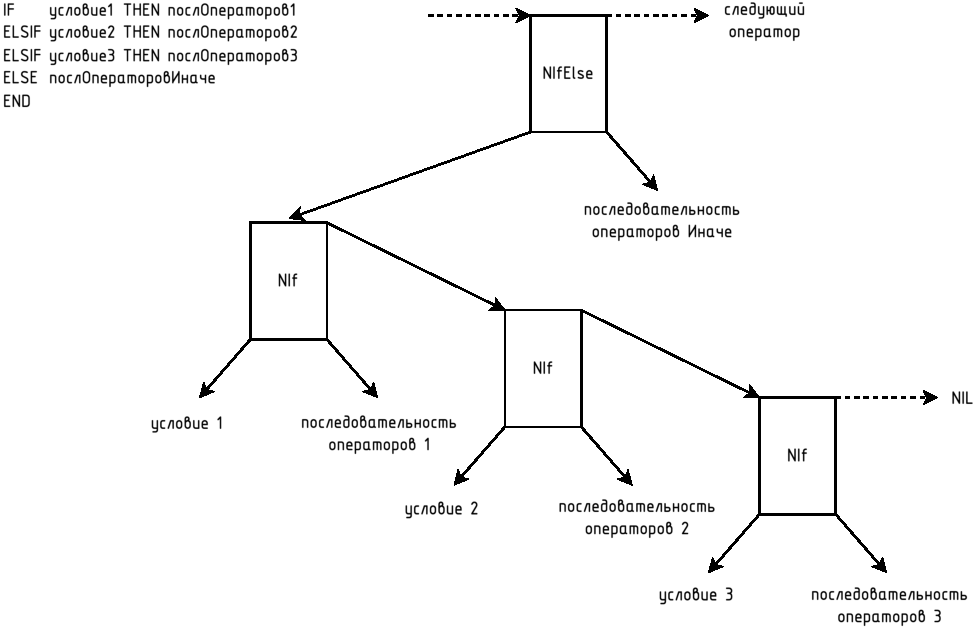
\includegraphics[width=\textheight,height=0.6\textwidth,keepaspectratio]{figures/ifelsif.pdf}
%\vspace{0.5cm}
\caption{Абстрактное синтаксическое дерево конструкции IF THEN ELSIF ELSE}
\label{fig:IfElsif}
\end{figure}

\end{minipage}}%
\end{center}
\newpage

\section{Генератор кода}

\firstparskip Генерация машинного кода относится к постпроцессору компилятора и технически выполнена в виде трёх модулей: обходчика дерева \code{Traverser}, испускателя машинного кода \code{Emitter} и низкоуровневый генератора \code{Generator}.

Обходчик получает подготовленное в препроцессоре абстрактное синтаксическое дерево. Это происходит только в том случае, если на этапе разбора исходного кода не возникло каких-либо ошибок. Общая координация организма компилятора осуществляется главным модулем \code{Moc}, который, собственно, и запускает препроцессор с постпроцессором.

Задача обходчика\tire обойти дерево в определённом порядке и на каждом этапе совершить соответствующий вызов процедуры модуля-испускателя. Испускатель, в свою очередь, вызовет необходимые процедуры генератора, в результате чего в массиве генератора будет набран соответствующий машинный код.

Модуль \code{Generator}, реализующий низкоуровневый генератор кода, и управляемый преимущественно модулем \code{Emitter}, имеет глобальную переменную \,\code{code: ARRAY maxCodeLen OF BYTE}\,, которая накапливает в себе производимый генератором машинный код. Для этого реализованы вспомогательные процедуры \code{Byte}, \code{Word}, \code{DWord}, \code{Set} и \code{String}\tire набор, очень похожий на соответствующий набор в компоновщике\footnote{См. с.~\pageref{Linker} настоящей работы.}. Но если там вывод идёт в файл, то здесь все переданные этим процедурам значения складываются в 
массив \code{code}.

Переменная \code{pc} (program counter) в том же модуле выполняет роль указателя на индекс массива \code{code}, куда будет записан следующий байт, или\tire что то же самое\tire количество байтов, уже записанных в \code{code}.

Модуль \code{Emitter} содержит по одной процедуре на генерацию каждой инструкции в машинном коде. Его процедуры вызываются обходчиком \code{Traverser}.

\section{Компоновщик}

\firstparskip Если в ходе работы постпроцессора ошибок не произошло (в качестве таковых можно предположить сбой постпроцессора или вызов его нереализованных частей), главный модуль вызывает компоновщик, выполненный в виде модуля \code{Linker}. Процедура компоновщика \code{Link} получает в качестве параметра только имя выходного исполнимого файла.

Задача компоновщика заключается в том, чтобы записать различные части исполнимого файла в соответствии с форматом, принятым на целевой вычислительной системе. В~нашем случае это операционная система macOS на базе процессора Apple Silicon, и формат файла называется Mach‑O.

Составные части файла, разумеется, должны быть согласованы между собой. Основной его компонент\tire машинный код целевого процессора\tire обычно размещается в середине файла. К~началу работы компоновщика итоговая длина машинного кода уже известна, а сам он находится в массиве модуля \code{Generator}, отвечающего за низкоуровневую генерацию.

\needspace{15\baselineskip}
Главная процедура компоновщика приведена в листинге~\ref{lst:Linker:Link}).

\captionsetup{type=listing}
\captionlisting{Главная процедура компоновщика}
\label{lst:Linker:Link}
\begin{modula2long}
PROCEDURE Link*(exeFname: ARRAY OF CHAR);
BEGIN
  Strings.Copy(exeFname, fname);
  codeLen := Generator.CodeLength();
  OpenOutputFile;
  IF ¬Machine.hadErrors THEN
    Output;
    IF Machine.hadErrors THEN
      Files.Close(F)
    ELSE
      Files.Register(F);
      ChmodAndSign
    END
  END
END Link;
\end{modula2long}

Для получения длины сгенерированного машинного кода в байтах вызывается функциональная процедура \code{Generator.CodeLength}. Затем последовательно, с проверкой ошибок, вызываются процедуры компоновщика \code{OpenOutputFile}, \code{Output} и \code{ChmodAndSign}.

Процедура \code{OpenOutputFile} (см. листинг~\ref{lst:Linker:OpenOutputFile}) открывает файл на запись. Имя файла было передано из главного модуля. Если файл открыть не удаётся, будет вызвана процедура сообщения об ошибке в модуле \code{Machine}. К~этому моменту модуль \code{Machine} уже будет переведён в фазу постпроцессора, поэтому ошибка будет выведена без указания положения в файле с исходным кодом. Это важно, поскольку ошибки фазы постпроцессора не связаны с конкретным исходным кодом.

\captionsetup{type=listing}
\captionlisting{Процедура компоновщика OpenOutputFile}
\label{lst:Linker:OpenOutputFile}
\begin{modula2long}
PROCEDURE OpenOutputFile;
BEGIN
  F := Files.New(fname);
  IF F = NIL THEN
    Machine.Error(Errors.outputFile)
  ELSE
    Files.Set(r, F, 0)
  END
END OpenOutputFile;
\end{modula2long}

Процедура \code{Output} (см. листинг~\ref{lst:Linker:Output}) осуществляет необходимые вызовы процедур, выводящие части исполнимого файла: заголовок (процедура \code{Header}), команды (процедура \code{Commands}), специфичные для формата \textit{Mach‑O} так называемые цепные фиксации (процедура \code{ChainedFixups}), префиксное дерево экспортированных объектов (процедура \code{ExportsTrie}), разметку процедур (процедура \code{FunctionStarts}) и символьную таблицу (процедура \code{SymbolTable}).

\captionsetup{type=listing}
\captionlisting{Процедура компоновщика Output}
\label{lst:Linker:Output}
\begin{modula2long}
PROCEDURE Output;
BEGIN
  Header;
  Commands;

  (* Zero-out until position 4000H - codeSpace *)
  Zeros(4000H - codeSpace - Files.Pos(r));
  (* Machine code *)
  Generator.Output(r);
  (* Unwind Info *)
  Zeros(codeSpace - codeLen);

  ChainedFixups;
  ExportsTrie;
  FunctionStarts;
  SymbolTable
END Output;
\end{modula2long}

Процедура \code{Commands} вызывает 16 других процедур: \code{Command0}, \code{Command1} и т.~д. (см. листинг~\ref{lst:Linker:Commands}).

\begin{listing}[H]
\caption{Процедура компоновщика Commands}
\vspace{-17pt}
\label{lst:Linker:Commands}
\begin{modula2}
(** Outputs Mach‑O commands to the file. *)
PROCEDURE Commands;
BEGIN
  Command0;
  Command1;
  (* ... *)
  Command15
END Commands;
\end{modula2}
\end{listing}

Из-за требований выравнивания в исполнимом файле присутствуют значительные области, заполненные нулями. Например, секция «unwind info», содержащая отладочную информацию, в текущей версии компилятора заполняется нулями, что не влияет на корректность работы скомпилированной программы.

Процедура \code{ChmodAndSign} (см. листинг~\ref{lst:Linker:ChmodAndSign}) выполняет два ключевых действия, необходимых для успешного запуска полученного исполнимого файла в операционной системе \textit{macOS}.

\begin{listing}[H]
\caption{Процедура компоновщика ChmodAndSign}
\vspace{-17pt}
\label{lst:Linker:ChmodAndSign}
\begin{modula2}
PROCEDURE ChmodAndSign;
VAR s: ARRAY 1024 OF CHAR;
  err: INTEGER;
BEGIN
  (* Chmod *)
  s := 'chmod +x ';
  Strings.Append(fname, s);
  err := Machine.Exec(s);
  IF err # 0 THEN
    Machine.Error(Errors.chmodFailed)
  ELSE
    (* Sign *)
    s := 'codesign -s - -f --timestamp=none ';
    Strings.Append(fname, s);
    err := Machine.Exec(s);
    IF err # 0 THEN
      Machine.Error(Errors.signFailed)
    END
  END
END ChmodAndSign;
\end{modula2}
\end{listing}

Во-первых, она вызывает команду \code{chmod} с параметром «\,\code{+x}\,», помечая файл в файловой системе как исполнимый. Это действие обязательно для всех UNIX-подобных систем. В~операционных системах Windows и DOS подобный шаг не требуется, поскольку исполнимость файла определяется по его расширению (\code{.EXE}, \code{.COM}, \code{.BAT}).

Во-вторых, процедура \code{ChmodAndSign} снабжает сгенерированный исполнимый файл цифровой подписью. Для этого она вызывает внешнюю утилиту \code{codesign}, которая доступна на всех современных версиях macOS. Без цифровой подписи запуск исполнимого файла будет заблокирован операционной системой. При этом, в целях безопасности, пользователю не будет отображено явное сообщение об ошибке.

Базовая подпись с помощью утилиты \code{codesign} может быть выполнена без участия в программе разработчика Apple, однако такая подпись не позволит обойти защиту Gatekeeper при распространении программ за пределами системы.

\label{Linker}

Компоновщик реализует вспомогательные процедуры \code{Byte}, \code{Word}, \code{DWord}, \code{QWord}, \code{Set}, \code{String} и \code{Zeros} (см. листинг~\ref{lst:Linker:HelperProcedures}), которые позволяют удобно осуществлять запись двоичных данных в файл.

% Breakable captioned listing (not a float)
\captionsetup{type=listing}
\captionlisting{Пример вспомогательных процедур компоновщика}
\label{lst:Linker:HelperProcedures}
\begin{modula2long}
(** Выводит 1 байт в файл. *)
PROCEDURE Byte(x: BYTE);
BEGIN
  Files.Write(r, x)
END Byte;

(** Выводит двойное слово = 4 байта в файл.
    Порядок байтов от младшего к старшему. *)
PROCEDURE DWord(x: INTEGER);
BEGIN
  Byte(x MOD 100H);
  Byte(x DIV 100H MOD 100H);
  Byte(x DIV 10000H MOD 100H);
  Byte(x DIV 1000000H MOD 100H)
END DWord;

(** Выводит множество в файл как 4 байта.
    Порядок байтов от младшего к старшему. *)
PROCEDURE Set(x: SET);
BEGIN
  DWord(ORD(x))
END Set;

(** Выводит строку в файл (однобайтовые литеры)
    с последующим добавлением нулевых байтов до
    достижения общего количества в n байт. Если n
    меньше длины строки, строка не усекается. *)
PROCEDURE String(s: ARRAY OF CHAR; n: INTEGER);
VAR i: INTEGER;
BEGIN
  i := 0;
  WHILE s[i] # 0X DO
    Byte(ORD(s[i]));
    INC(i)
  END;
  WHILE i < n DO
    Byte(0);
    INC(i)
  END
END String;

(** Выводит n нулевых байтов в файл. *)
PROCEDURE Zeros(n: INTEGER);
BEGIN
  WHILE n > 0 DO
    Byte(0);
    DEC(n)
  END
END Zeros;
\end{modula2long}

С процедуры \code{Header} начинается запись в исполнимый файл. Она представлена в~листинге~\ref{lst:Linker:Header}. Все записывающие процедуры компоновщика выглядят подобным образом. Они построены с использованием документации формата Mach‑O и по результатам экспериментальных данных\footnote{См. гл.~\ref{sec:MachOExperiment} на с.~\pageref{sec:MachOExperiment} настоящей работы.}.

\captionsetup{type=listing}
\captionlisting{Процедура вывода заголовка файла Mach‑O}
\label{lst:Linker:Header}
\begin{modula2long}
(** Выводит первые 32 байта - заголовок Mach‑O - в файл. *)
PROCEDURE Header;
BEGIN
  (* Магическое число FEED-FACF,
  порядок байтов от младшего к старшему *)
  Byte(0CFH); Byte(0FAH); Byte(0EDH); Byte(0FEH);
  (* Тип ЦПУ = ARM64 *)
  DWord(100000CH);
  (* Подтип ЦПУ = ARM64_ALL *)
  DWord(0);
  (* Тип файла = MH_EXECUTE *)
  DWord(2);
  (* Количество команд загрузки *)
  DWord(15);
  (* Размер команд загрузки в байтах *)
  DWord(744-16);
  (* Флаги = {NOUNDEFS, DYLDLINK, TWOLEVEL, PIE} *)
  Set({0, 2, 7, 21});
  (* Зарезервировано = 0 *)
  DWord(0)
END Header;
\end{modula2long}

\needspace{8\baselineskip}
\subsection{Использование типа SET}

\firstparskip Обыкновенно флаги обозначаются в виде целого числа в шестнадцатеричной записи и составляются с помощью поразрядной операции ИЛИ:

\begin{center}
\code{0x00200085 = 0x1 | 0x4 | 0x80 | 0x200000}
\end{center}

Запись числа в виде \code{0x200000} не несёт никакой смысловой нагрузки, кроме того, что это константа, которая подлежит сцеплению с другими подобными константами посредством поразрядных операций.

\label{OberonSets}

В Обероне, а ранее в Модуле‑2, существует тип \code{SET}. Это не тот же тип \code{SET}, который был в Паскале. В~Обероне он определяется как множество небольших целых чисел~\cite[с.~29]{WirthPIO}. Количество этих чисел фактически определяется архитектурой целевой вычислительной системы, так как важно добиться, чтобы операции над множествами могли быть эффективно реализованы как поразрядные (битовые) операции. Характерная для современных систем мощность такого множества равна 32. На более старых системах\tire 16, на некоторых новых\tire 64. Чаще всего она равна машинному слову в битах. Идея типа данных, который бы на более высоком уровне абстракции использовал компактное представление массива булевых значений как битовых множеств, используя математически привлекательные концепции.

Никлаус Вирт указывает, что идея этого типа данных принадлежит Чарльзу Энтони Ричарду Хоару~\cite{WirthSet}. Она возникла из попытки поднять такие типы, как Bits и Bitset, на более высокий уровень математически привлекательной абстракции.

Синтаксически в языке Оберон значение (литерал) типа \code{SET} задаётся с помощью фигурных скобок:

\begin{center}
\code{\{0, 1, 5..8, 15\}}
\end{center}

На машинном уровне такое множество будет представлять собой 4 байта памяти, в которых биты-единицы будут обозначать присутствие соответствующего элемента в множестве.

Таким образом, для представления флагов \code{0x00200085} в Обероне будет использована запись $\{0, 2, 7, 21\}$. Такая запись делает наглядным и тот факт, что флагов четыре. По записи \code{0x00200085} это не сразу видно, так как цифра 5 обозначает два флага ($4 + 1$).

Фактически, каждое число в фигурных скобках означает количество нулей, которое надо отступить справа в записи числа в его двоичной форме, прежде чем поставить единицу. Или, что то же самое, число два, возведённое в степень номера элемента. Таким образом, множество $\{0\}$ означает число \code{0x00000001}, множество $\{1\}$\tire число \code{0x00000002}, множество $\{2\}$\tire \code{0x00000004} и так далее. Удобство множеств по сравнению с шестнадцатеричными числовыми флагами становится особенно наглядным при использовании больших чисел. Число \code{0x00200000} в виде множества представляется как короткое~$\{21\}$.

\section{Особенности архитектуры Apple~Silicon}

\firstparskip Как уже указывалось ранее, исполнимые файлы в операционной системе macOS имеют формат Mach‑O. Ключевой составляющей исполнимого файла является сегмент, содержащий машинный код, непосредственно предназначенный для исполнения на целевой архитектуре. Рассмотрим принципы построения этого машинного кода.

Архитектура ARM64, лежащая в основе процессоров Apple Silicon, использует фиксированный размер инструкции: каждая инструкция занимает ровно 4 байта, то есть 32 бита. Это свойство отличает её от архитектур с переменной длиной инструкций (например, x86), и существенно упрощает как аппаратное декодирование команд, так и анализ машинного кода человеком. Следует отметить, что 64-битная разрядность архитектуры относится не к длине инструкции, а к ширине регистров общего назначения и адресного пространства. Таким образом, инструкции остаются компактными, несмотря на расширенные возможности.

Фиксированная длина инструкций в ARM64 упрощает задачу визуального анализа: каждое двойное слово (4 байта) в шестнадцатеричном выводе машинного кода можно с уверенностью интерпретировать как инструкцию. Для сравнения, архитектура x86 и её 64-битное расширение x86\_64 используют переменную длину инструкций\tire от 1 до 15 байт~\cite{x86and64},\tire что приводит к сложности синхронизации при анализе кода с произвольного адреса, так как делает границы между инструкциями неочевидными.

Примером может служить следующий фрагмент кода ARM64:

{\small\begin{verbatim}
  9100 0400    mov x0, #0x20
  D280 0021    mov x1, #0x1
\end{verbatim}}

Здесь легко увидеть, что каждая строка представляет собой ровно одну инструкцию\tire 4 байта, 8 шестнадцатеричных цифр.

Кроме того, ARM64 построена по принципам RISC (Reduced Instruction Set Computer), что означает ограниченный набор инструкций, более простое и предсказуемое их поведение, отсутствие скрытых побочных эффектов и ориентацию на однотипные форматы команд. Это делает архитектуру особенно удобной для компиляторов, которые могут с высокой степенью детерминированности формировать машинный код без необходимости глубокого анализа сложных инструкций или их комбинаций, как в случае CISC-архитектур (к~которым относится, например, x86).

ARM64 в контексте проектирования компилятора предоставляет значительные преимущества: как в части генерации кода, так и в части анализа его корректности, особенно на этапе отладки или обучения.

\subsection{Инструкции, регистры и соглашения}

\firstparskip Архитектура ARM64 использует набор инструкций A64, введённый в спецификации ARMv8-A. A64 является RISC-набором инструкций, в котором каждая команда выполняет простую операцию. Инструкции делятся на несколько категорий:

1.\hspace{0.5em}Арифметико-логические операции: \code{ADD}, \code{SUB}, \code{AND}, \code{ORR}, \code{EOR}, \code{LSL}, \code{LSR}, \code{ASR}.

2.\hspace{0.5em}Операции с ОЗУ: \code{LDR}, \code{STR}, \code{LDUR}, \code{STUR}, \code{LDP}, \code{STP}.

3.\hspace{0.5em}Управление потоком исполнения: \code{B}, \code{BL}, \code{RET}, \code{BR}, \code{CBZ}, \code{CBNZ}, \code{TBZ}, \code{TBNZ}.

4.\hspace{0.5em}Системные инструкции: \code{MSR}, \code{MRS}, \code{NOP}, \code{ISB}, \code{DSB}, \code{DMB}.

ARM64 предоставляет 31 универсальный 64-битный регистр общего назначения (\code{X0}---\code{X30}) и специальный регистр \code{SP} (stack pointer). Также доступны 32 векторных регистра (\code{V0}–\code{V31}) для операций с плавающей запятой и SIMD\footnote{SIMD означает Single Instruction, Multiple Data\tire одна инструкция, множество данных.}.

В соответствии с AAPCS64 (Procedure Call Standard for the ARM 64-bit Architecture), параметры функций передаются через регистры \code{X0}---\code{X7}, а возвращаемое значение\tire через \code{X0}. Регистры \code{X19}---\code{X28} являются сохраняемыми вызываемой процедурой (callee-saved) и должны быть восстановлены к моменту возврата из процедуры. Регистр \code{X30} (\code{LR}) используется для хранения адреса возврата~\cite{AAPCS64}.

\needspace{14\baselineskip}
\paragraph{Пример.} Рассмотрим простую функцию на языке Оберон:

\begin{modula2}
PROCEDURE Add(a, b: INTEGER): INTEGER;
RETURN a + b END Add;
\end{modula2}

Компилятор может транслировать её в следующий A64-код:

{\samepage
{\small\begin{verbatim}
add:
    ADD X0, X0, X1
    RET
\end{verbatim}}

Здесь параметры \code{a} и \code{b} передаются через \code{X0} и \code{X1}, результат возвращается в \code{X0}.
}

\subsection{Особенности системных вызовов на macOS}

\firstparskip Архитектура системных вызовов в macOS построена на основе ядра XNU (X is Not Unix), сочетающего элементы Mach, BSD и IOKit. Несмотря на внешнее сходство с Unix-подобными системами, системные вызовы macOS имеют ряд отличий, как в интерфейсе, так и в реализации.

На архитектуре ARM64 системные вызовы осуществляются с помощью инструкции \code{svc \#0} (Supervisor Call). Эта инструкция инициирует переход в привилегированный режим и передаёт управление ядру. Номер системного вызова и его аргументы передаются в регистрах согласно соглашению AAPCS64, принятому в среде Darwin.

Для системных вызовов в macOS используются правила, идентичные обычным процедурным вызовам:

1) регистр \code{X16} содержит номер системного вызова;

2) аргументы передаются в регистрах \code{X0}---\code{X7};

3) возвращаемое значение помещается в \code{X0};

4) ошибки указываются через значение в \code{X0} и код \code{errno}.

\needspace{16\baselineskip}
\textbf{Пример.} Вызов функции \code{write(fd, buffer, size)} на уровне системного интерфейса выглядит следующим образом:

\begin{asm}
mov  x0, #1           ; дескриптор (stdout)
adr  x1, buffer        ; указатель на буфер
mov  x2, #13          ; длина
mov  x16, #0xFFFF    ; системный селектор (магическое
                       ;                        значение для Apple)
mov  x8, #0x2000004 ; номер системного вызова write
svc  #0               ; собственно вызов
\end{asm}

Здесь \code{0x2000004}\tire это системный номер функции \code{write} в пространстве вызовов macOS. Префикс \code{0x2000000} означает, что это системный вызов BSD (в отличие от Mach или IOKit).

В отличие от Linux, где системные вызовы обычно реализованы через \code{svc \#0} с номерами без префикса (например, \code{write = 64} на ARM64), macOS использует уникальную схему нумерации и дополнительные селекторы. Более того, взаимодействие с ядром в macOS часто происходит не напрямую, а через обёртки в \code{libSystem.dylib}, которые реализуют стандарт POSIX API.

Для генерации нативного кода под macOS компилятор должен учитывать особенности соглашения вызова системных функций, специфику нумерации и структуру передачи параметров. Неправильная реализация интерфейса системных вызовов приводит к ошибкам исполнения или некорректному взаимодействию с ядром. В~связи с этим понимание механизма системных вызовов Darwin ABI имеет ключевое значение при проектировании постпроцессора компилятора.

\needspace{16\baselineskip}
\section{Исследование формата файла Mach‑O}

\label{sec:MachOExperiment}

\firstparskip

Рассмотрим исполнимый файл «\code{01\_exit}», который можно получить из объектного файла при помощи следующей команды:

{\small\begin{verbatim}
ld 01_exit.o -o 01_exit -lSystem -syslibroot
    `xcrun -sdk macosx --show-sdk-path` -e _start
\end{verbatim}}

Воспользуемся для исследования инструментом «MachO\-View»\tire графической программой, отображающей содержимое файлов Mach‑O в удобном виде. Первые 32 байта представляют собой заголовок Mach-0: (см. рис.~\ref{fig:MachOHeader}).

\begin{figure}[H]
\centering
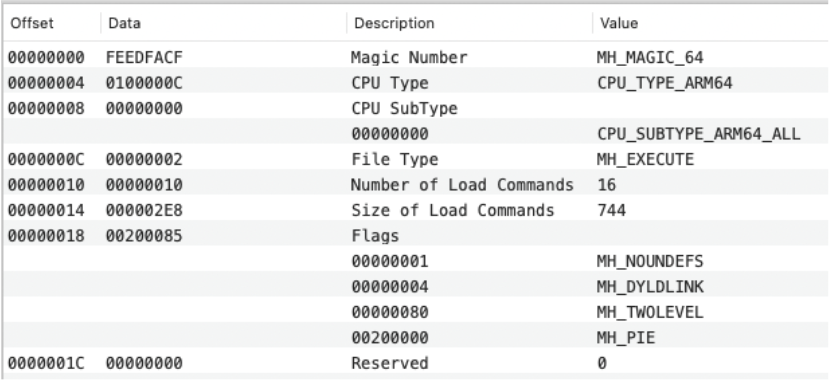
\includegraphics[width=\textwidth]{figures/machoheader.png}
\caption{Заголовок Mach‑O}
\label{fig:MachOHeader}
\end{figure}

Заголовок Mach64 (первые 32 байта).

По смещению $1\,016$ видим количество команд загрузки, а именно $16$. В~простейшем \textit{объектном} файле их было бы $4$. По смещению $1\,416$ видим значение $744$. Это суммарный размер всех команд загрузки в байтах.

Если в объектном файле все флаги были бы сняты (значение \code{Flags} было равно нулю), то в исполнимом файле оно равно $20\,008\,516$, что соответствует четырём флагам со значениями $2^0$, $2^2$, $2^7$ и $2^{21}$. Вот их значения:

\par\vspace{\baselineskip}\noindent
$2^0$\;=\;\code{NOUNDEFS}~---~файл не содержит неопределённых символов; \\
$2^2$\;=\;\code{DYLDLINK}\;---\;файл собран для работы с динамическим компоновщиком; \\
$2^7$\;=\;\code{TWOLEVEL}\;---\;используется двухуровневая система именования символов; \\
$2^{21}$\;=\;\code{PIE}\;---\;исполнимый файл является позиционно-незави\-си\-мым.

\paragraph{Двухуровневая система именования символов.}

В отличие от системы плоского пространства имён (Flat Namespace) двухуровневая система именования символов (Two-Level Name\-space) в Mach‑O позволяет избежать конфликтов между библиотеками (фреймворками), если они определяют символы с одинаковыми именами, поскольку двухуровневая система с каждым символом соотносит конкретную динамическую библиотеку.

\paragraph{Команды загрузки.}

После заголовка в файле Mach‑O идёт указанное количество команд загрузки. Некоторые команды определяют целые сегменты в ОЗУ, а другие несут вспомогательную информацию. В~исполнимом файле, который мы рассматриваем, объявлено 3 сегмента.

Первый из них\tire «\,\code{\_\_PAGEZERO}» (см. рис.~\ref{fig:Command0})\tire занимает в виртуальной памяти 4~Гбайт и, в общем-то, в этом и заключается его предназначение. Он явно закрывает эту память от доступа со стороны приложения, т.~к. не определяет в сегменте ни одной секции.

\begin{figure}[H]
\centering
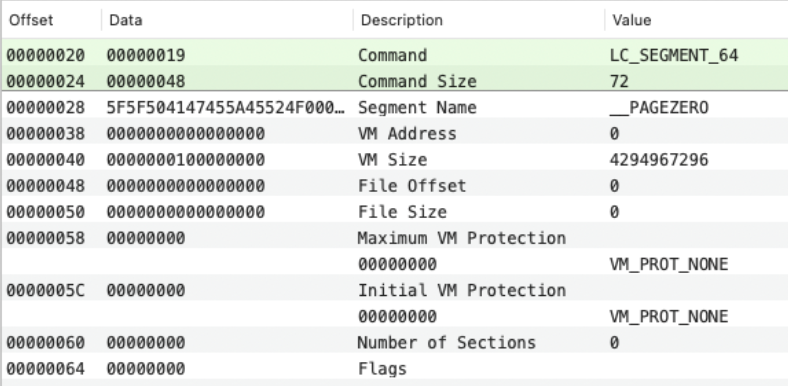
\includegraphics[width=\textwidth]{figures/command0.png}
\caption{Сегмент №~0}
\label{fig:Command0}
\end{figure}

Второй сегмент носит имя «\,\code{\_\_TEXT}» (см. рис.~\ref{fig:Command1}) и в нашем случае занимает $88$ байта. Содержимое этого фрагмента памяти будет заполнено $88$ байтами из файла по смещению $16\,296$.

\begin{figure}[H]
\centering
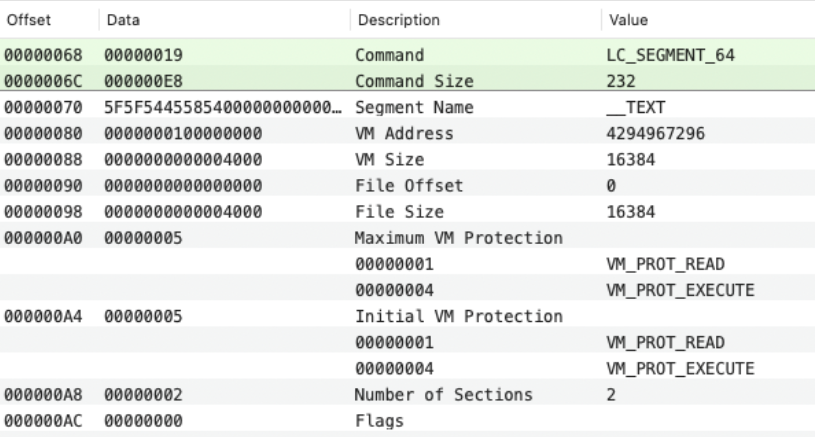
\includegraphics[width=\textwidth]{figures/command1.png}
\caption{Сегмент №~1}
\label{fig:Command1}
\end{figure}

Третий сегмент носит имя «\,\code{\_\_LINKEDIT}» (см. рис.~\ref{fig:Command2}) и выполняет массу служебных релей. В нашем случае данный сегмент занимает $16\,384$ байта. Содержимое этого сегмента памяти будет заполнено первыми $16\,384$ байтами из файла.

\begin{figure}[H]
\centering
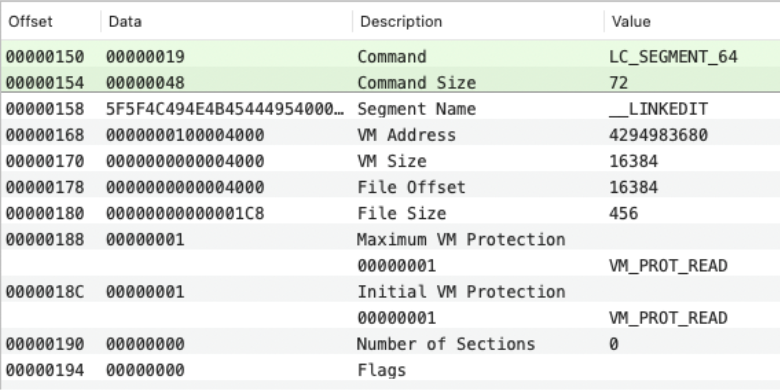
\includegraphics[width=\textwidth]{figures/command2.png}
\caption{Сегмент №~2}
\label{fig:Command2}
\end{figure}

Рассматривая команды загрузки Mach‑O одну за другой, внося изменения в бинарный файл, можно изучить этот формат на практике, что и было сделано при изготовлении данного компилятора.

\section*{Заключение}
\addcontentsline{toc}{section}{Заключение}

В ходе выполненной работы была достигнута поставленная цель\tire создан нативный компилятор языка Оберон для процессоров Apple Silicon (ARM64) под macOS, полностью реализующий все этапы преобразования исходного кода: лексический и синтаксический анализ, проверку типов, построение промежуточного представления, генерацию машинного кода и компоновку исполняемого файла в формате Mach‑O.

Для начального «раскручивания» компилятора на macOS/ARM64 была портирована среда Free Oberon и транслятор Оберона в Си Ofront+, при этом были исправлены ошибки в передаче REAL-параметров по ABI ARM64. В результате получен работоспособный прототип, пригодный не только для практического использования, но и для дальнейшего развития\tire в том числе готовый к перенацеливанию на другие архитектуры, внедрения оптимизаций и расширения функциональности.

Разработанный инструмент может служить наглядным учебным материалом при изучении технологий построения компиляторов и особенностей ARM64-машинного кода, а его исходные тексты легко интегрируются в открытые образовательные и исследовательские проекты.

В перспективе целесообразно расширить возможности компилятора за счёт:

1) внедрения фаз оптимизации кода;

2) поддержки различных диалектов Оберон;

3) автоматизации процесса сборки под различные ОС и аппаратные платформы;

4) проведения сравнительных тестов производительности (бенчмарков);

5) создание автоматической системы распространения компонентов.

Таким образом, работа не только закрыла пробел в экосистеме Оберона на Apple Silicon, но и заложила прочную основу для её дальнейшего развития и применения в образовательных и исследовательских целях.

Исходный код компилятора опубликован в GitHub-репозитории \href{https://github.com/kekcleader/moc}{github.com/kekcleader/moc}
и на сайте
\href{https://moc.oberon.org}{moc.oberon.org}.


\clearpage\literatura{bibliography}

\newpage

\appendix
\appsection{Синтаксис Оберона}
\label{appendix:OberonSyntax}

\newenvironment{hanging}{
  \begin{list}{}{
    \setlength{\leftmargin}{2em}
    \setlength{\itemindent}{-2em}
    \setlength{\parsep}{0pt}
  }
  \item[]
}{
  \end{list}
}


%\begin{flushleft}
%{\setlength{\parindent}{0pt}
{\small
\begin{verbatim}
буква = "A" | "B" | ... | "Z" | "a" | "b" | ... | "z".
цифра = "0" | "1" | "2" | "3" | "4" | "5" | "6" | "7" |
        "8" | "9".
шестнЦифра = цифра | "A" | "B" | "C" | "D" | "E" | "F".
идент = буква {буква | цифра}.
уточнИдент = [идент "."] идент.
идентОпр = идент ["*"].
целое = цифра {цифра} | цифра {шестнЦифра} "H".
вещественное = цифра {цифра} "." {цифра} [порядок].
порядок = ("E") ["+" | "-"] цифра {цифра}.
число = целое | вещественное.
строка = """ {литера} """ | цифра {шестнЦифра} "X".
ОбъявлениеКонстанты = идентОпр "=" КонстантноеВыражение.
КонстантноеВыражение = выражение.
ОбъявлениеТипа = идентОпр "=" тип.
тип = уточнИдент | ТипМассив | ТипЗапись | ТипУказатель |
      ПроцедурныйТип.
ТипМассив = ARRAY длина {"," длина} OF тип.
длина = КонстантноеВыражение.
ТипЗапись = RECORD ["(" БазовыйТип ")"]
            [ПоследСпискаПолей] END.
БазовыйТип = уточнИдент.
ПоследСпискаПолей = СписокПолей {";" СписокПолей}.
СписокПолей = СписокИдент ":" тип.
СписокИдент = идентОпр {"," идентОпр}.
ТипУказатель = POINTER TO тип.
ПроцедурныйТип = PROCEDURE [ФормальныеПараметры].
ОбъявлениеПеременных = СписокИдент ":" тип.
выражение = ПростоеВыражение [отношение ПростоеВыражение].
отношение = "=" | "#" | "<" | "<=" | ">" | ">=" | IN | IS.
ПростоеВыражение = ["+"|"-"] выражение
                   {ОперацияСложения выражение}.
ОперацияСложения = "+" | "-" | OR.
выражение = множитель {ОперацияУмножения множитель}.
ОперацияУмножения = "*" | "/" | DIV | MOD | "&".
множитель = число | строка | NIL | TRUE | FALSE |
множество | обозначение [ФактическиеПараметры] |
"(" выражение ")" | "¬" множитель.
обозначение = уточнИдент {селектор}.
селектор = "." идент | "[" СписокВыражений "]" |
           "↑" | "(" уточнИдент ")".
множество = "{" [элемент {"," элемент}] "}".
элемент = выражение [".." выражение].
СписокВыражений = выражение {"," выражение}.
ФактическиеПараметры = "(" [СписокВыражений] ")".
оператор = [присваивание | ВызовПроцедуры  |
            ОператорЕсли | ОператорВыбора  |
            ОператорПока | ОператорПовтора | ОператорFor].
присваивание = обозначение ":=" выражение
ВызовПроцедуры = обозначение [ФактическиеПараметры].
ПослОператоров = оператор {";" оператор}.
ОператорЕсли = IF выражение THEN ПослОператоров
               {ELSIF выражение THEN ПослОператоров}
               [ELSE ПослОператоров] END.
ОператорВыбора = CASE выражение OF вариант
                 {" | " вариант} END.
вариант = [СписокМетокВарианта ":" ПослОператоров].
СписокМетокВарианта = МеткиВарианта {"," МеткиВарианта }.
МеткиВарианта = метка [".." метка].
метка = целое | строка | уточнИдент.
ОператорПока = WHILE выражение DO ПослОператоров
               {ELSIF выражение DO ПослОператоров} END.
ОператорПовтора = REPEAT ПослОператоров UNTIL выражение.
ОператорFor = FOR идент ":=" выражение TO выражение
[BY КонстантноеВыражение] DO ПослОператоров END.
ОбъявлениеПроцедуры = ЗаголовокПроцедуры ";"
                      ТелоПроцедуры идент.
ЗаголовокПроцедуры = PROCEDURE идентОпр
                     [ФормальныеПараметры].
ТелоПроцедуры = ПослОбъявлений [BEGIN ПослОператоров]
[RETURN выражение] END.
ПослОбъявлений = [CONST {ОбъявлениеКонстант ";"}]
                 [TYPE {ОбъявлениеТипов ";"}]
                 [VAR {ОбъявлениеПеременных ";"}]
                 {ОбъявлениеПроцедуры ";"}.
ФормальныеПараметры = "(" [СекцияФП {";" СекцияФП }] ")"
                      [":" уточнИдент].
СекцияФП = [VAR] идент {"," идент} ":" ФормалныйТип.
ФормалныйТип = {ARRAY OF} уточнИдент.
модуль = MODULE идент ";" [СписокИмпорта] ПослОбъявлений
         [BEGIN ПослОператоров] END идент ".".
СписокИмпорта = IMPORT импорт {"," импорт} ";".
импорт = [идент ":="] идент.
\end{verbatim}
}
%}
%\end{flushleft}


\newpage

\appendix
\appsection{Исходный~код~компилятора}
\label{appendix:CompilerSource}

% Переопределяем окружение modula2long с меньшим шрифтом для приложения
\renewenvironment{modula2long}{\VerbatimEnvironment\begin{minted}[linenos,numbersep=8pt,fontsize=\small,frame=lines,framesep=6pt,style=bw,breaklines=true,breakanywhere=true,encoding=utf8,xleftmargin=0pt,xrightmargin=0pt,texcomments=false,mathescape=false,commandchars=none]{text}}{\end{minted}}

\addcontentsline{toc}{subsection}{Модуль Moc (главный модуль)}
\captionsetup{type=listing}
\captionlisting{Полный исходный текст модуля Moc (главный модуль)}
\label{lst:ModuleMoc}
\vspace{10pt}
\begin{modula2long}
MODULE Moc;
IMPORT Out, Args, Strings, Machine, Parser,
        Scanner, Traverser, Table, Tree, Linker;
CONST
  version = '1.0.0-alpha.1';

PROCEDURE Welcome;
BEGIN
  Out.String('Mac Oberon Compiler version ');
  Out.String(version); Out.Ln;
  Out.String('Copyright (c) 2025');
  Out.String(' by Arthur Yefimov.'); Out.Ln
END Welcome;

PROCEDURE Usage;
VAR s: ARRAY 256 OF CHAR;
BEGIN
  Out.String('Usage:'); Out.Ln; Args.Get(0, s);
  Out.String(' '); Out.String(s);
  Out.String(' {parameter} sourceFile'); Out.Ln; Out.Ln;
  Out.String('Parameters:'); Out.Ln;
  Out.String(' -o outputFile    Specify an executable file name'); Out.Ln;
  Out.String(' --debug          Enable debug output'); Out.Ln; Out.Ln
END Usage;

(** Finds period and truncates the string there. Puts the result in exe.
    'Module.Mod' -> 'Module'.
    If period is not found, the result is an empty string. *)
PROCEDURE SourceToExeFname(fname: ARRAY OF CHAR;
                                VAR exe: ARRAY OF CHAR);
VAR i: INTEGER;
BEGIN
  i := 0;
  WHILE (fname[i] # 0X) & (fname[i] # '.') DO
    exe[i] := fname[i];
    INC(i)
  END;
  IF fname[i] = 0X THEN i := 0 END;
  exe[i] := 0X
END SourceToExeFname;

PROCEDURE ParseArgs(VAR mainFname, exeFname: ARRAY OF CHAR);
VAR i, count: INTEGER;
  s: ARRAY 256 OF CHAR;
  ok: BOOLEAN;
BEGIN
  ok := TRUE;
  mainFname := '';
  exeFname := '';
  i := 1;
  count := Args.Count();
  WHILE i <= count DO
    Args.Get(i, s);
    IF s = '-o' THEN
      Args.Get(i + 1, exeFname);
      INC(i)
    ELSIF s = '--debug' THEN
      Machine.SetDebug(TRUE)
    ELSIF mainFname = '' THEN
      Strings.Copy(s, mainFname)
    ELSE
      ok := FALSE
    END;
    INC(i)
  END;
  IF ¬ok THEN
    Out.String('Error while parsing command line arguments. ');
    Usage
  ELSIF exeFname = '' THEN
    SourceToExeFname(mainFname, exeFname)
  END
END ParseArgs;

PROCEDURE Run(mainFname, exeFname: ARRAY OF CHAR);
VAR module: Tree.Node;
BEGIN
  IF ¬Machine.OpenSourceFile(mainFname) THEN
    Out.String('Could not open source file "');
    Out.String(mainFname); Out.String('".'); Out.Ln
  ELSE
    module := Parser.Parse();
    IF ¬Machine.hadErrors THEN
      Machine.BackendPhase;
      IF Machine.debugFrontend THEN
        Out.String('--- Abstract Syntax Tree ---'); Out.Ln;
        Tree.Print(module, 0);
        Out.String('--- Symbol Table ---'); Out.Ln;
        Table.Print(Table.topScope, 0)
      END;

      Traverser.SetAddressesAndSizes(Table.topScope);
      IF ¬Machine.hadErrors THEN
        Traverser.Traverse(module);
        IF ¬Machine.hadErrors THEN
          Linker.Link(exeFname)
        END
      END
    END
  END
END Run;

PROCEDURE PraseAndRun;
VAR
  mainFname, exeFname: ARRAY 256 OF CHAR;
BEGIN
  ParseArgs(mainFname, exeFname);
  IF mainFname # '' THEN
    Run(mainFname, exeFname)
  ELSE
    Out.String('No file specified.'); Out.Ln
  END
END PraseAndRun;

PROCEDURE Do*;
BEGIN
  IF Args.Count() = 0 THEN
    Welcome;
    Usage
  ELSE
    PraseAndRun
  END
END Do;

BEGIN
  Do
END Moc.
\end{modula2long}


\addcontentsline{toc}{subsection}{Модуль Machine (загрузка текста)}
\captionsetup{type=listing}\captionlisting{Полный исходный текст модуля Machine (загрузка текста)}\begin{modula2long}
MODULE Machine;
IMPORT Out, Errors := MocErrors, Files, Utf8, Platform, SYSTEM;

CONST
  maxInt* = 2147483647; (** Maximum integer value, 32-bit *)
  maxExp* = 38; (** Maximum exponent of a real value *)

  pointerSize* = 8; (** In bytes *)

  debugFrontend* = TRUE;

  compilerName* = 'moc';

  (** compilationPhase values **)
  frontend* = 1;
  backend*  = 2;

TYPE
  SHORTCHAR = SYSTEM.CHAR8;

  Pos* = RECORD
    line*, col*: INTEGER
  END;

VAR
  fname: ARRAY 256 OF CHAR;
  r: Files.Rider;
  prevChar: CHAR;
  pos*: Pos; (** Current position in the source file being read *)
  errorPos*: Pos; (** Position of the last error. If no errors, line = -1 *)
  hadErrors*: BOOLEAN; (** TRUE after a call to Error *)

  debug: BOOLEAN;
  compilationPhase: INTEGER; (** For proper error output, see constants *)

(** Begins output of an error if its position is different from the last one.
    Returns true on success and false if the position is the same. *)
PROCEDURE BeginError(): BOOLEAN;
VAR ok: BOOLEAN;
BEGIN
  hadErrors := TRUE;
  ok := TRUE;
  IF compilationPhase = backend THEN
    Out.String(compilerName);
    Out.String(': error: ')
  ELSIF (pos.line # errorPos.line) OR (pos.col # errorPos.col) THEN
    Out.String(fname); Out.Char(':');
    Out.Int(pos.line, 0); Out.Char(':');
    Out.Int(pos.col, 0); Out.String(': error: ');
    errorPos := pos
  ELSE
    ok := FALSE
  END
RETURN ok END BeginError;

PROCEDURE Error*(errno: INTEGER);
VAR s: ARRAY 256 OF CHAR;
BEGIN
  IF BeginError() THEN
    Errors.Message(errno, s);
    Out.String(s); Out.Ln
  END
END Error;

PROCEDURE ErrorExpected*(symExpected, symFound: INTEGER);
BEGIN
  IF BeginError() THEN
    Errors.PrintSymbol(symExpected);
    Out.String(' expected, but ');
    Errors.PrintSymbol(symFound);
    Out.String(' found');
    Out.Ln
  END
END ErrorExpected;

PROCEDURE ErrorExpectedMsg*(errno, symFound: INTEGER);
VAR s: ARRAY 256 OF CHAR;
BEGIN
  IF BeginError() THEN
    Errors.Message(errno, s);
    Out.String(s);
    Out.String(', but ');
    Errors.PrintSymbol(symFound);
    Out.String(' found');
    Out.Ln
  END
END ErrorExpectedMsg;

PROCEDURE NotImplemented*(feature: ARRAY OF CHAR);
VAR s: ARRAY 256 OF CHAR;
BEGIN
  IF BeginError() THEN
    Errors.Message(Errors.notImplemented, s);
    Out.String(s); Out.String(': ');
    Out.String(feature); Out.Ln
  END
END NotImplemented;

(** Returns next character from the file opened. On end of file return 0X.
    Keeps track of the current position in the file in terms of line:column. *)
PROCEDURE Read*(VAR ch: CHAR);
BEGIN
  IF r.eof THEN
    ch := 0X
  ELSE
    IF prevChar = 0AX THEN
      INC(pos.line);
      pos.col := 1
    ELSE
      INC(pos.col)
    END;
    Files.ReadChar(r, prevChar);
    ch := prevChar
  END
END Read;

PROCEDURE OpenSourceFile*(filename: ARRAY OF CHAR): BOOLEAN;
VAR F: Files.File;
BEGIN
  F := Files.Old(filename);
  IF F = NIL THEN
    fname := ''
  ELSE
    fname := filename;
    Files.Set(r, F, 0);
    prevChar := 0X
  END;
  pos.line := 1;
  pos.col := 1;
  errorPos.line := -1;
  hadErrors := F = NIL;
  compilationPhase := frontend
RETURN ¬hadErrors END OpenSourceFile;

PROCEDURE Exec*(command: ARRAY OF CHAR): INTEGER;
VAR z: ARRAY 4096 OF SHORTCHAR;
BEGIN
  Utf8.Encode(command, z);
RETURN  Platform.System(z) END Exec;

PROCEDURE BackendPhase*;
BEGIN
  compilationPhase := backend
END BackendPhase;

PROCEDURE SetDebug*(value: BOOLEAN);
BEGIN
  debug := value
END SetDebug;

BEGIN
  debug := FALSE
END Machine.
\end{modula2long}

\needspace{15\baselineskip}

\addcontentsline{toc}{subsection}{Модуль Scanner (лексический анализатор)}
\captionsetup{type=listing}\captionlisting{Полный исходный текст модуля Scanner (лексический анализатор)}\begin{modula2long}
MODULE Scanner;
IMPORT Out, Machine, Errors := MocErrors;

CONST
  identSize = 256;
  stringSize = 1024;

  uptoChar = 7FX; (** Used as a fix for double dot right after a digit *)

  (** Lexical symbols **)
  null        =  0;      times*      =  1;      rdiv*     =  2;      div*     =  3;
  mod*       =  4;      and*       =  5;      plus*     =  6;      minus*  =  7;
  or*         =  8;      eql*       =  9;      neq*      = 10;      lss*     = 11;
  leq*        = 12;      gtr*       = 13;      geq*       = 14;     in*       = 15;
  is*         = 16;      arrow*     = 17;      period*    = 18;     char*    = 20;
  int*        = 21;      real*       = 22;     false*     = 23;     true*    = 24;
  nil*         = 25;     string*     = 26;     not*       = 27;     lparen*  = 28;
  lbrak*      = 29;     lbrace*     = 30;     ident*     = 31;      if*       = 32;
  while*      = 34;     repeat*    = 35;      case*     = 36;      for*     = 37;
  comma*    = 40;      colon*     = 41;      becomes* = 42;      upto*    = 43;
  rparen*    = 44;      rbrak*    = 45;      rbrace*   = 46;      then*   = 47;
  of*        = 48;      do*        = 49;      to*       = 50;      by*      = 51;
  semicolon* = 52;      end*       = 53;      bar*      = 54;     else*     = 55;
  elsif*      = 56;      until*      = 57;      return*   = 58;     array*    = 60;
  record*    = 61;      pointer*    = 62;      const*    = 63;     type*     = 64;
  var*       = 65;      procedure* = 66;      begin*    = 67;      import*  = 68;
  module*    = 69;      eot*       = 70;

TYPE
  Ident* = ARRAY identSize OF CHAR;
  StrVal* = ARRAY stringSize OF CHAR;

VAR
  (** Results of Get **)
  name*: Ident;
  intVal*: INTEGER;
  realVal*: REAL;
  strVal*: StrVal;
  strLen*: INTEGER;

  (** - **)
  ch: CHAR; (** Read-ahead character *)

(** Converts an uppercase hexadecimal digit to an integer. *)
PROCEDURE HexToInt(c: CHAR): INTEGER;
VAR n: INTEGER;
BEGIN
  IF ('0' <= c) & (c <= '9') THEN
    n := ORD(c) - ORD('0')
  ELSIF ('A' <= c) & (c <= 'F') THEN
    n := ORD(c) - (ORD('A') + 10)
  ELSE
    ASSERT(FALSE)
  END
RETURN n END HexToInt;

(** Reports whether ch is a decimal digit. *)
PROCEDURE IsDigit(): BOOLEAN;
RETURN ('0' <= ch) & (ch <= '9')
END IsDigit;

(** Reports whether ch is an uppercase hexadecimal digit (0..F). *)
PROCEDURE IsHex(): BOOLEAN;
RETURN IsDigit() OR ('A' <= ch) & (ch <= 'F')
END IsHex;

(** Reports whether ch is a letter. *)
PROCEDURE IsAlpha(): BOOLEAN;
RETURN ('A' <= ch) & (ch <= 'Z') OR
       ('a' <= ch) & (ch <= 'z') OR
       (ch = '_')
END IsAlpha;

(** Reports whether ch is a letter or a number. *)
PROCEDURE IsAlphaNum(): BOOLEAN;
RETURN IsAlpha() OR IsDigit()
END IsAlphaNum;

(** Examines name and returns one of keyword lexical symbol constants,
    or ident if name is not a keyword. Uses the passed in actual length
    of name for speed. *)
PROCEDURE IdentifyKeyword(len: INTEGER): INTEGER;
VAR sym: INTEGER;
BEGIN
  sym := ident;
  IF len = 2 THEN
    IF    name = "OR" THEN sym := or
    ELSIF name = "IN" THEN sym := in
    ELSIF name = "IS" THEN sym := is
    ELSIF name = "IF" THEN sym := if
    ELSIF name = "OF" THEN sym := of
    ELSIF name = "DO" THEN sym := do
    ELSIF name = "TO" THEN sym := to
    ELSIF name = "BY" THEN sym := by
    END
  ELSIF len = 3 THEN
    IF    name = "END" THEN sym := end
    ELSIF name = "VAR" THEN sym := var
    ELSIF name = "NIL" THEN sym := nil
    ELSIF name = "DIV" THEN sym := div
    ELSIF name = "MOD" THEN sym := mod
    ELSIF name = "FOR" THEN sym := for
    END
  ELSIF len = 4 THEN
    IF    name = "THEN" THEN sym := then
    ELSIF name = "ELSE" THEN sym := else
    ELSIF name = "TRUE" THEN sym := true
    ELSIF name = "TYPE" THEN sym := type
    ELSIF name = "REAL" THEN sym := real
    ELSIF name = "CASE" THEN sym := case
    END
  ELSIF len = 5 THEN
    IF    name = "ELSIF" THEN sym := elsif
    ELSIF name = "FALSE" THEN sym := false
    ELSIF name = "CONST" THEN sym := const
    ELSIF name = "WHILE" THEN sym := while
    ELSIF name = "ARRAY" THEN sym := array
    ELSIF name = "BEGIN" THEN sym := begin
    ELSIF name = "UNTIL" THEN sym := until
    END
  ELSIF len = 6 THEN
    IF    name = "RETURN" THEN sym := return
    ELSIF name = "RECORD" THEN sym := record
    ELSIF name = "REPEAT" THEN sym := repeat
    ELSIF name = "IMPORT" THEN sym := import
    ELSIF name = "MODULE" THEN sym := module
    END
  ELSIF (len = 7) & (name = "POINTER")   THEN sym := pointer
  ELSIF (len = 9) & (name = "PROCEDURE") THEN sym := procedure
  END
RETURN sym END IdentifyKeyword;

(** Skips a possibly nested comment. Precondition: ch = '*'. *)
PROCEDURE SkipComment;
VAR prevCh: CHAR;
BEGIN
  prevCh := 0X;
  Machine.Read(ch);
  WHILE (ch # 0X) & ¬((prevCh = '*') & (ch = ')')) DO
    prevCh := ch;
    Machine.Read(ch);
    IF (prevCh = '(') & (ch = '*') THEN (* Nested comment *)
      SkipComment
    END
  END;
  IF ch # 0X THEN Machine.Read(ch) END
END SkipComment;

PROCEDURE ReadNumber(VAR sym: INTEGER);
VAR i, len: INTEGER;
  ok: BOOLEAN;
  err: INTEGER;
  digits: ARRAY 16 OF INTEGER;

  PROCEDURE DecimalToInt(digits: ARRAY OF INTEGER; len: INTEGER);
  VAR i: INTEGER;
    err: INTEGER;
  BEGIN
    err := Errors.none;
    intVal := 0;
    i := 0;
    REPEAT
      IF digits[i] >= 10 THEN
        err := Errors.badInt
      ELSE
        (* Overflow check *)
        IF intVal > (Machine.maxInt - digits[i]) DIV 10 THEN
          err := Errors.intOverflow
        ELSE
          intVal := intVal * 10 + digits[i]
        END
      END;
      INC(i)
    UNTIL i = len;
    IF err # Errors.none THEN
      intVal := 0;
      Machine.Error(err)
    END
  END DecimalToInt;

  (** Returns 10 in the power of e. *)
  PROCEDURE Ten(e: INTEGER): REAL;
  VAR x, t: REAL;
  BEGIN
    x := 1.0;
    t := 10.0;
    WHILE e > 0 DO
      IF ODD(e) THEN x := t * x END;
      t := t * t;
      e := e DIV 2
    END
  RETURN x END Ten;

  PROCEDURE ReadReal(digits: ARRAY OF INTEGER; len: INTEGER);
  VAR i, exponent, scale: INTEGER;
    negE: BOOLEAN;
    ok: BOOLEAN;
  BEGIN
    ok := TRUE;
    realVal := 0.0;
    exponent := 0;
    (* Integer part *)
    i := 0;
    REPEAT
      IF digits[i] >= 10 THEN
        ok := FALSE
      ELSE
        realVal := realVal * 10.0 + FLT(digits[i])
      END;
      INC(i)
    UNTIL i = len;
    IF ¬ok THEN
      realVal := 0.0;
      Machine.Error(Errors.badReal)
    END;
    (* Fraction part *)
    WHILE IsDigit() DO
      realVal := realVal * 10.0 + FLT(ORD(ch) - ORD('0'));
      DEC(exponent);
      Machine.Read(ch)
    END;
    (* Scale factor *)
    IF (ch = 'E') OR (ch = 'D') THEN
      Machine.Read(ch);
      scale := 0; 
      IF ch = '-' THEN
        Machine.Read(ch);
        negE := TRUE
      ELSE
        negE := FALSE;
        IF ch = '+' THEN Machine.Read(ch) END
      END;
      IF ¬IsDigit() THEN
        Machine.Error(Errors.noDigit)
      ELSE
        REPEAT
          scale := scale * 10 + ORD(ch) - ORD('0');
          Machine.Read(ch)
        UNTIL ¬IsDigit();
        IF negE THEN DEC(exponent, scale) ELSE INC(exponent, scale) END
      END
    END;
    IF exponent < 0 THEN
      IF exponent >= -Machine.maxExp THEN
        realVal := realVal / Ten(-exponent)
      ELSE
        realVal := 0.0
      END
    ELSIF exponent > 0 THEN
      IF exponent <= Machine.maxExp THEN
        realVal := Ten(exponent) * realVal
      ELSE
        Machine.Error(Errors.largeExponent);
        realVal := 0.0
      END
    END
  END ReadReal;

BEGIN
  ok := TRUE;
  len := 0;
  REPEAT
    IF len # LEN(digits) THEN
      digits[len] := HexToInt(ch);
      INC(len)
    ELSE
      ok := FALSE
    END;
    Machine.Read(ch)
  UNTIL ¬IsHex();
  IF ¬ok THEN
    Machine.Error(Errors.manyDigits)
  END;
  IF (ch = 'H') OR (ch = 'X') THEN (* Hexadecimal integer or char *)
    ok := TRUE;
    intVal := 0;
    i := 0;
    REPEAT (* TODO Allow negative two's compliment HEX constants *)
      (* Overflow check *)
      IF intVal > (Machine.maxInt - digits[i]) DIV 16 THEN
        ok := FALSE
      ELSE
        intVal := intVal * 16 + digits[i]
      END;
      INC(i)
    UNTIL i = len;
    IF ¬ok THEN
      intVal := 0;
      Machine.Error(Errors.intOverflow)
    END;
    IF ch = 'X' THEN sym := char ELSE sym := int END;
    Machine.Read(ch)
  ELSIF ch = '.' THEN (* Real number or integer + upto *)
    Machine.Read(ch);
    IF ch = '.' THEN (* Upto (..) right after a digit *)
      ch := uptoChar; (* Fix for Get to read upto symbol instead of period *)
      DecimalToInt(digits, len);
      sym := int
    ELSE
      ReadReal(digits, len);
      sym := real
    END
  ELSE (* Decimal integer *)
    DecimalToInt(digits, len);
    sym := int
  END
END ReadNumber;

PROCEDURE Get*(VAR sym: INTEGER);
VAR i: INTEGER;
  closeCh: CHAR;
  ok, comment: BOOLEAN;
BEGIN
  REPEAT
    sym := null;
    comment := FALSE;
    WHILE (ch # 0X) & (ch <= ' ') DO Machine.Read(ch) END;
    IF ch = 0X THEN
      sym := eot
    ELSIF IsAlpha() THEN (* Also '_' *)
      name[0] := ch;
      Machine.Read(ch);
      ok := TRUE;
      i := 1;
      WHILE IsAlphaNum() DO
        IF i = LEN(name) - 1 THEN
          ok := FALSE
        ELSE
          name[i] := ch;
          INC(i)
        END;
        Machine.Read(ch)
      END;
      name[i] := 0X;
      IF ¬ok THEN
        Machine.Error(Errors.longIdent);
        name := ''
      END;
      sym := IdentifyKeyword(i)
    ELSIF IsDigit() THEN
      ReadNumber(sym)
    ELSIF (ch = '"') OR (ch = "'") THEN
      closeCh := ch;
      Machine.Read(ch);
      ok := TRUE;
      strLen := 0;
      WHILE (ch >= ' ') & (ch # closeCh) DO
        IF strLen = LEN(strVal) - 1 THEN
          ok := FALSE
        ELSE
          strVal[strLen] := ch;
          INC(strLen)
        END;
        Machine.Read(ch)
      END;
      strVal[strLen] := 0X;
      IF ch < ' ' THEN
        Machine.Error(Errors.unclosedStr);
        strVal := '';
        strLen := 0
      ELSE
        Machine.Read(ch);
        IF ¬ok THEN
          Machine.Error(Errors.longStr);
          strVal := '';
          strLen := 0
        END
      END;
      sym := string
    ELSIF ch < '0' THEN (* '!'..'/' *)
      IF    ch = '#' THEN Machine.Read(ch); sym := neq
      ELSIF ch = '&' THEN Machine.Read(ch); sym := and
      ELSIF ch = '(' THEN
        Machine.Read(ch);
        IF ch = '*' THEN
          SkipComment;
          comment := TRUE
        ELSE
          sym := lparen
        END
      ELSIF ch = ')' THEN Machine.Read(ch); sym := rparen
      ELSIF ch = '*' THEN Machine.Read(ch); sym := times
      ELSIF ch = '+' THEN Machine.Read(ch); sym := plus
      ELSIF ch = ',' THEN Machine.Read(ch); sym := comma
      ELSIF ch = '-' THEN Machine.Read(ch); sym := minus
      ELSIF ch = '.' THEN
        Machine.Read(ch);
        IF ch = '.' THEN Machine.Read(ch); sym := upto ELSE sym := period END
      ELSIF ch = '/' THEN Machine.Read(ch); sym := rdiv
      END (* ELSE ! $ % *)
    ELSIF ch < 'A' THEN (* ':'..'@' *)
      IF ch = ':' THEN
        Machine.Read(ch);
        IF ch = '=' THEN Machine.Read(ch); sym := becomes ELSE sym := colon END
      ELSIF ch = ';' THEN Machine.Read(ch); sym := semicolon
      ELSIF ch = '<' THEN
        Machine.Read(ch);
        IF ch = '=' THEN Machine.Read(ch); sym := leq ELSE sym := lss END
      ELSIF ch = '=' THEN Machine.Read(ch); sym := eql
      ELSIF ch = '>' THEN
        Machine.Read(ch);
        IF ch = '=' THEN Machine.Read(ch); sym := geq ELSE sym := gtr END
      END (* ELSE ? @ *)
    ELSIF ch < 'a' THEN (* '['..'`' *)
      IF    ch = '[' THEN Machine.Read(ch); sym := lbrak
      ELSIF ch = ']' THEN Machine.Read(ch); sym := rbrak
      ELSIF ch = '↑' THEN Machine.Read(ch); sym := arrow
      END (* ELSE \ ` *)
    ELSIF ch = '{' THEN Machine.Read(ch); sym := lbrace
    ELSIF ch = '|' THEN Machine.Read(ch); sym := bar
    ELSIF ch = '}' THEN Machine.Read(ch); sym := rbrace
    ELSIF ch = '¬' THEN Machine.Read(ch); sym := not
    ELSIF ch = uptoChar THEN Machine.Read(ch); sym := upto
    END;
    IF ¬comment & (sym = null) THEN
      Machine.Read(ch);
      Machine.Error(Errors.badChar)
    END
  UNTIL sym # null (* Comment *)
END Get;

PROCEDURE Init*;
BEGIN
  Machine.Read(ch)
END Init;

END Scanner.
\end{modula2long}


\addcontentsline{toc}{subsection}{Модуль Parser (синтаксический анализатор)}
\captionsetup{type=listing}\captionlisting{Полный исходный текст модуля Parser (синтаксический анализатор)}\begin{modula2long}
MODULE Parser;
IMPORT Out, Strings, Table, Tree, Machine, S := Scanner, Builder,
  Errors := MocErrors, Kernel;

TYPE
  Ident = S.Ident;

VAR
  sym: INTEGER; (** Read-ahead symbol *)

  modName: Ident;
  dummy: Table.Object;

PROCEDURE TestScanner;
BEGIN
  WHILE sym # S.eot DO
    IF sym = S.string THEN
      Out.String('string [');
      Out.Int(S.strLen, 0); Out.String("] '");
      Out.String(S.strVal); Out.Char("'")
    ELSIF sym = S.int THEN
      Out.String('int ');
      Out.Int(S.intVal, 0)
    ELSIF sym = S.real THEN
      Out.String('real ');
      Out.Real(S.realVal, 0)
    ELSIF sym = S.ident THEN
      Out.String('ident ');
      Out.String(S.name)
    ELSE
      Errors.PrintSymbol(sym)
    END;
    S.Get(sym);
    Out.Ln
  END;
  Out.String('eot'); Out.Ln
END TestScanner;

(** Reports whether sym is the expected symbol. If not, reports an error. *)
PROCEDURE Check(expectedSym: INTEGER): BOOLEAN;
BEGIN
  IF sym # expectedSym THEN
    Machine.ErrorExpected(expectedSym, sym)
  END
RETURN sym = expectedSym END Check;

(** Checks that sym is the expected symbol and skips it, or reports an error. *)
PROCEDURE Skip(expectedSym: INTEGER);
BEGIN
  IF sym = expectedSym THEN
    S.Get(sym)
  ELSE
    Machine.ErrorExpected(expectedSym, sym)
  END
END Skip;

(** If sym is the expected symbol then skips it and returns true,
    otherwise returns false. *)
PROCEDURE Skipped(expectedSym: INTEGER): BOOLEAN;
VAR ok: BOOLEAN;
BEGIN
  ok := sym = expectedSym;
  IF ok THEN S.Get(sym) END
RETURN ok END Skipped;

PROCEDURE StandardProcedureCall(x: Tree.Node): Tree.Node;
BEGIN
  Machine.NotImplemented('standard procedure call')
RETURN x END StandardProcedureCall;

(** qualident = [ident "."] ident. *)
PROCEDURE Qualident(): Table.Object;
VAR object: Table.Object;
BEGIN
  object := Table.ThisObject(S.name);
  S.Get(sym); (* ident *)
  IF object = NIL THEN
    Machine.Error(Errors.undefinedIdent);
    object := dummy
  END;

  IF (object.class = Table.Mod) & Skipped(S.period) THEN
    IF ¬Check(S.ident) THEN
      object := dummy
    ELSE
      object := Table.ThisImport(object, S.name);
      S.Get(sym); (* ident *)
      IF object = NIL THEN
        Machine.Error(Errors.undefinedIdent);
        object := dummy
      END
    END
  END
RETURN object END Qualident;

PROCEDURE ↑ Expression(): Tree.Node;

(** designator = qualident {selector}.
     selector = "." ident | "[" ExpList "]" | "↑" | "(" qualident ")". *)
PROCEDURE Designator(): Tree.Node;
VAR designator: Tree.Node;
  qualident: Table.Object;
BEGIN
  qualident := Qualident();
  designator := Builder.NewLeaf(qualident);
  IF designator.class # Table.SProc THEN
    (* Selectors *)
    WHILE sym = S.lbrak DO (* Array index *)
      Machine.NotImplemented('array index');
      REPEAT S.Get(sym) UNTIL (sym = S.eot) OR (sym = S.rbrak);
      S.Get(sym) (* rbrak, TODO *)
    ELSIF sym = S.period DO (* Record field *)
      S.Get(sym); (*TODO*)
      Machine.NotImplemented('record field')
    ELSIF sym = S.arrow DO (* Pointer dereference *)
      S.Get(sym); (*TODO*)
      Machine.NotImplemented('pointer dereference')
    ELSIF (sym = S.lparen) & (* Type guard *)
          (designator.type.form IN {Table.Record, Table.Pointer})
    DO
      Machine.NotImplemented('type guard');
      REPEAT S.Get(sym) UNTIL (sym = S.eot) OR (sym = S.rparen);
      Skip(S.rparen) (*TODO*)
    END
  END
RETURN designator END Designator;

(** ActualParameters = "(" [ExpList] ")".
     ExpList = expression {"," expression}.
     Precondition: sym = S.lparen *)
PROCEDURE ActualParameters(procedure: Tree.Node;
  formal: Table.Object): Tree.Node;
VAR actual, list, last: Tree.Node;
  n, paramCount: INTEGER;
BEGIN
  Skip(S.lparen);
  n := 0;
  paramCount := procedure.object.type.paramCount;
  IF sym # S.rparen THEN
    actual := Expression();
    IF formal = NIL THEN
      Machine.Error(Errors.manyArguments);
    ELSE
      Builder.Param(actual, formal);
      list := actual;
      last := list;
      formal := formal.next;
      INC(n);
      WHILE Skipped(S.comma) DO
        actual := Expression();
        IF formal # NIL THEN
          Builder.Param(actual, formal);
          last.link := actual;
          formal := formal.next;
        END;
        INC(n)
      END
    END
  END;
  IF n < paramCount THEN
    Machine.Error(Errors.fewArguments)
  ELSIF n > paramCount THEN
    Machine.Error(Errors.manyArguments)
  END;
  Skip(S.rparen)
RETURN list END ActualParameters;

(** ProcedureCall = designator [ActualParameters].
     Precondition: designator already read. *)
PROCEDURE ProcedureCall(designator: Tree.Node): Tree.Node;
VAR formalParams: Table.Object;
  actualParams, x: Tree.Node;
BEGIN
  IF (designator.class # Tree.NProc) OR
     (designator.object.type.form # Table.Proc) THEN
    Machine.Error(Errors.notProcedure)
  ELSIF designator.object.constVal.intVal > 0 THEN (* Standard procedure *)
    IF designator.object.class = Table.SFunc THEN
      Machine.Error(Errors.procCallFunc)
    ELSE (* class = SProc *)
      x := StandardProcedureCall(designator)
    END
  ELSE (* Non-standard procedure *)
    formalParams := Builder.PrepareCall(designator);
    IF sym = S.lparen THEN
      actualParams := ActualParameters(designator, formalParams)
    END;
    IF designator.type.base.form # Table.NoType THEN
      Machine.Error(Errors.procCallFunc)
    END;
    x := Builder.Call(designator, actualParams, formalParams)
  END
RETURN x END ProcedureCall;

(** factor = number | string | NIL | TRUE | FALSE |
    set | designator [ActualParameters] | "(" expression ")" | "¬" factor. *)
PROCEDURE Factor(): Tree.Node;
VAR x, y: Tree.Node;
  op: INTEGER;
  qualident, formalParams: Table.Object;
  actualParams: Tree.Node;
BEGIN
  (* Sync *)
  IF (sym < S.char) OR (sym > S.ident) THEN
    Machine.ErrorExpectedMsg(Errors.noExpression, sym);
    REPEAT S.Get(sym) UNTIL (sym >= S.char) & (sym <= S.for) OR (sym >= S.then)
  END;

  IF sym = S.ident THEN
    x := Designator();
    IF (x.class = Tree.NProc) & (x.object.class = Table.SFunc) THEN
      x := StandardProcedureCall(x)
    ELSIF Skipped(S.lparen) & (x.type.form = Table.Proc) &
          (x.type.base.form # Table.NoType)
    THEN
      formalParams := Builder.PrepareCall(x);
      actualParams := ActualParameters(x, formalParams);
      Skip(S.rparen);
      x := Builder.Call(x, actualParams, formalParams)
    END
  ELSIF sym = S.int THEN
    x := Builder.NewIntConst(S.intVal);
    S.Get(sym)
  ELSIF sym = S.char THEN
    x := Builder.NewIntConst(S.intVal);
    x.type := Table.charType;
    S.Get(sym)
  ELSIF sym = S.real THEN
    x := Builder.NewRealConst(S.realVal);
    S.Get(sym)
  ELSIF Skipped(S.not) THEN
    x := Factor();
    x := Builder.MonadicOperator(S.not, x)
  (*TODO true, false, string, nil, etc.*)
  ELSIF Skipped(S.lparen) THEN (* Subexpression *)
    x := Expression();
    Skip(S.rparen)
  ELSE
    Machine.Error(Errors.noFactor);
    S.Get(sym);
    x := Builder.NewIntConst(0)
  END
RETURN x END Factor;

(** term = factor {MulOperator factor}.
     MulOperator = "*" | "/" | DIV | MOD | "&". *)
PROCEDURE Term(): Tree.Node;
VAR x, y: Tree.Node;
  op: INTEGER;
BEGIN
  x := Factor();
  (* {MulOperator factor} *)
  WHILE (S.times <= sym) & (sym <= S.and) DO
    op := sym;
    S.Get(sym); (* op *)
    y := Factor();
    x := Builder.DyadicOperator(op, x, y)
  END
RETURN x END Term;

(** SimpleExpression = ["+" | "-"] term {AddOperator term}.
     AddOperator = "+" | "-" | OR. *)
PROCEDURE SimpleExpression(): Tree.Node;
VAR x, y: Tree.Node;
  op: INTEGER;
BEGIN
  (* ["+" | "-"] term *)
  IF sym = S.minus THEN
    S.Get(sym);
    x := Term();
    x := Builder.MonadicOperator(S.minus, x)
  ELSE
    IF sym = S.plus THEN S.Get(sym) END;
    x := Term()
  END;
  (* {AddOperator term} *)
  WHILE (S.plus <= sym) & (sym <= S.or) DO
    op := sym;
    S.Get(sym); (* op *)
    y := Term();
    x := Builder.DyadicOperator(op, x, y)
  END
RETURN x END SimpleExpression;

(** expression = SimpleExpression [relation SimpleExpression].
     relation = "=" | "#" | "<" | "<=" | ">" | ">=" | IN | IS. *)
PROCEDURE Expression(): Tree.Node;
VAR x, y: Tree.Node;
  relation: INTEGER;
BEGIN
  x := SimpleExpression();
  IF (S.eql <= sym) & (sym <= S.geq) THEN
    relation := sym;
    S.Get(sym); (* relation *)
    y := SimpleExpression();
    x := Builder.DyadicOperator(relation, x, y)
  ELSIF sym = S.in THEN
    Machine.NotImplemented('operator IN')
  ELSIF sym = S.is THEN
    Machine.NotImplemented('operator IS')
  END
RETURN x END Expression;

(** assignment = designator ":=" expression.
     Precondition: designator and ":=" already read. *)
PROCEDURE Assignment(designator: Tree.Node): Tree.Node;
VAR assign, expr: Tree.Node;
BEGIN
  expr := Expression();
  assign := Tree.NewNode(Tree.NAssign);
  assign.subclass := Tree.assign;
  assign.left := designator;
  assign.right := expr
RETURN assign END Assignment;

(** IfStatement = IF expression THEN StatementSequence
    {ELSIF expression THEN StatementSequence}
    [ELSE StatementSequence] END. *)
PROCEDURE IfStatement(): Tree.Node;
VAR if: Tree.Node;
BEGIN

RETURN if END IfStatement;

(** WhileStatement = WHILE expression DO StatementSequence
    {ELSIF expression DO StatementSequence} END. *)
PROCEDURE WhileStatement(): Tree.Node;
VAR while: Tree.Node;
BEGIN

RETURN while END WhileStatement;

(** RepeatStatement = REPEAT StatementSequence UNTIL expression. *)
PROCEDURE RepeatStatement(): Tree.Node;
VAR repeat: Tree.Node;
BEGIN

RETURN repeat END RepeatStatement;

(** statement = [assignment | ProcedureCall | IfStatement | CaseStatement |
    WhileStatement | RepeatStatement | ForStatement]. *)
PROCEDURE Statement(): Tree.Node;
VAR statement, designator: Tree.Node;
BEGIN
  IF sym = S.ident THEN (* Assignment or procedure call *)
    designator := Designator();
    IF Skipped(S.becomes) THEN
      statement := Assignment(designator)
    ELSE
      statement := ProcedureCall(designator)
    END
  ELSIF Skipped(S.if) THEN
    statement := IfStatement()
  ELSIF Skipped(S.while) THEN
    statement := WhileStatement()
  ELSIF sym = S.case THEN
    Machine.NotImplemented('case statement')
  ELSIF sym = S.repeat THEN
    Machine.NotImplemented('repeat statement')
  ELSIF sym = S.for THEN
    Machine.NotImplemented('for statement')
  END
RETURN statement END Statement;

(** StatementSequence = statement {";" statement}. *)
PROCEDURE StatementSequence(): Tree.Node;
VAR first, prev, statement: Tree.Node;
BEGIN
  (* Sync *)
  IF ¬((sym >= S.ident) & (sym <= S.for) OR (sym >= S.semicolon)) THEN
    Machine.Error(Errors.noStatement);
    REPEAT S.Get(sym) UNTIL (sym >= S.ident)
  END;

  WHILE sym = S.semicolon DO S.Get(sym) END;
  first := Statement();
  prev := first;
  WHILE Skipped(S.semicolon) DO
    WHILE sym = S.semicolon DO S.Get(sym) END;
    statement := Statement();
    prev.link := statement;
    prev := statement
  END
RETURN first END StatementSequence;

(** ConstExpression = expression. *)
PROCEDURE ConstExpression(): Tree.Node;
VAR const: Tree.Node;
BEGIN
  const := Expression();
  IF const.class # Tree.NConst THEN
    Machine.Error(Errors.notConstant);
    const := Builder.NewIntConst(0)
  END
RETURN const END ConstExpression;

(** ConstDeclaration = identdef "=" ConstExpression.
     identdef = ident. *)
PROCEDURE ConstDeclaration;
VAR expr: Tree.Node;
  obj: Table.Object;
BEGIN
  obj := Table.NewObject(S.name, Table.Const);
  S.Get(sym); (* ident *)
  IF Skipped(S.eql) THEN
    expr := ConstExpression();
    IF expr.class # Tree.NConst THEN
      Machine.Error(Errors.notConstant)
    ELSE
      obj.type := expr.type;
      obj.constVal := expr.constVal
    END
  END
END ConstDeclaration;

(** type = qualident | ArrayType | RecordType | PointerType | ProcedureType.
     ArrayType = ARRAY length {"," length} OF type.
     length = ConstExpression.
     RecordType = RECORD ["(" BaseType ")"] [FieldListSequence] END.
     BaseType = qualident. *)
PROCEDURE Type(): Table.Type;
VAR obj: Table.Object;
  type: Table.Type;
BEGIN
  IF sym = S.ident THEN
    obj := Qualident();
    IF obj.class # Table.Typ THEN
      Machine.Error(Errors.notType)
    ELSIF (obj.type = NIL) OR (obj.type.form = Table.NoType) THEN
      Machine.Error(Errors.undefinedType)
    ELSE
      type := obj.type
    END
  ELSIF sym = S.array THEN
    Machine.NotImplemented('type array')
  ELSIF sym = S.record THEN
    Machine.NotImplemented('type record')
  ELSIF sym = S.pointer THEN
    Machine.NotImplemented('type pointer')
  ELSIF sym = S.procedure THEN
    Machine.NotImplemented('procedure type')
  ELSE
    Machine.Error(Errors.noType)
  END
RETURN type END Type;

(** TypeDeclaration = identdef "=" type. *)
PROCEDURE TypeDeclaration;
BEGIN
  Machine.NotImplemented('type declaration');
  (* Sync to VAR, BEGIN, RETURN or END *)
  REPEAT
    S.Get(sym)
  UNTIL (sym = S.var) OR (sym = S.begin) OR (sym = S.return) OR (sym = S.end)
END TypeDeclaration;

(** Reads a comma-spearated identifier list, adds an object of the given
    class for each identifier and returns the first created object.
     IdentList = identdef {"," identdef}.
     identdef = ident. *)
PROCEDURE IdentList(class: INTEGER): Table.Object;
VAR first, obj: Table.Object;
BEGIN
  first := Table.NewObject(S.name, class);
  S.Get(sym); (* ident *)
  WHILE sym = S.comma DO
    S.Get(sym); (* comma *)
    obj := Table.NewObject(S.name, class);
    S.Get(sym) (* ident *)
  END
RETURN first END IdentList;

(** VariableDeclaration = IdentList ":" type. *)
PROCEDURE VariableDeclaration;
VAR first: Table.Object;
  type: Table.Type;
BEGIN
  first := IdentList(Table.Var);
  Skip(S.colon);
  type := Type();
  WHILE first # NIL DO
    first.type := type;
    first := first.next
  END
END VariableDeclaration;

(** DeclarationSequence = [CONST {ConstDeclaration ";"}]
    [TYPE {TypeDeclaration ";"}] [VAR {VariableDeclaration ";"}]
    {ProcedureDeclaration ";"}. *)
PROCEDURE DeclarationSequence(): Tree.Node;
VAR procedures: Tree.Node;
BEGIN
  (* Sync *)
  IF (sym < S.const) & (sym # S.end) & (sym # S.return) THEN
    Machine.Error(Errors.noDeclaration);
    REPEAT
      S.Get(sym)
    UNTIL (sym >= S.const) OR (sym = S.end) OR (sym = S.return)
  END;

  IF Skipped(S.const) THEN
    WHILE sym = S.ident DO
      ConstDeclaration();
      Skip(S.semicolon)
    END
  END;

  IF Skipped(S.type) THEN
    WHILE sym = S.ident DO
      TypeDeclaration();
      Skip(S.semicolon)
    END
  END;

  IF Skipped(S.var) THEN
    WHILE sym = S.ident DO
      VariableDeclaration();
      Skip(S.semicolon)
    END
  END
RETURN procedures END DeclarationSequence;

(** FormalParameters = "(" [FPSection {";" FPSection}] ")" [":" qualident].
     FPSection = [VAR] ident {"," ident} ":" FormalType.
     FormalType = {ARRAY OF} qualident. *)

(** ProcedureDeclaration = ProcedureHeading ";" ProcedureBody ident.
     ProcedureHeading = PROCEDURE identdef [FormalParameters].
     ProcedureBody = DeclarationSequence [BEGIN StatementSequence]
    [RETURN expression] END.
     identdef = ident. *)

(** import = ident [":=" ident]. *)
PROCEDURE Import;
VAR name: Ident;
BEGIN
  IF Check(S.ident) THEN
    Strings.Copy(S.name, name);
    S.Get(sym);
    IF Skipped(S.becomes) THEN
      Table.Import(name, S.name, modName);
      S.Get(sym)
    ELSE
      Table.Import(name, name, modName)
    END
  END
END Import;

(** module = MODULE ident ";" [ImportList]
    DeclarationSequence [BEGIN StatementSequence] END ident ".".
     ImportList = IMPORT import {"," import} ";". *)
PROCEDURE Module(): Tree.Node;
VAR module: Tree.Node;
  name: Ident;
  procedures, statementSequence: Tree.Node;
BEGIN
  Skip(S.module);
  IF Check(S.ident) THEN
    Strings.Copy(S.name, modName);
    S.Get(sym); (* ident *)

    (* IMPORT *)
    Skip(S.semicolon);
    IF Skipped(S.import) THEN
      Import;
      WHILE Skipped(S.comma) DO
        Import
      END;
      Skip(S.semicolon)
    END;

    (* CONST, TYPE, VAR and BEGIN *)
    procedures := DeclarationSequence();
    IF Skipped(S.begin) THEN
      statementSequence := StatementSequence()
    END;

    module := Builder.Enter(procedures, statementSequence, NIL);
    Skip(S.end);
    IF Check(S.ident) THEN
      IF S.name # modName THEN
        Machine.Error(Errors.modNameMismatch)
      ELSE
        S.Get(sym); (* ident *)
        Skip(S.period)
      END
    END
  END
RETURN module END Module;

PROCEDURE Parse*(): Tree.Node;
VAR module: Tree.Node;
BEGIN
  S.Init;
  S.Get(sym);
  Table.Init;
  module := Module()
RETURN module END Parse;

BEGIN
  NEW(dummy);
  dummy.class := Table.Var;
  dummy.type := Table.intType
END Parser.
\end{modula2long}


\addcontentsline{toc}{subsection}{Модуль Table (таблица символов)}
\captionsetup{type=listing}\captionlisting{Полный исходный текст модуля Table (таблица символов)}\begin{modula2long}
MODULE Table;
IMPORT Out, Strings, Machine, Errors := MocErrors, Scanner;

CONST
  (** Object.class values **)
  Head* = 0; Const* = 1; Var*    = 2; VarPar* = 3; Field* = 4;
  Typ*  = 5; SProc* = 6; SFunc* = 7; Mod*     = 8;

  (** Type.form values **)
  Byte*  =  1; Bool*    =  2; Char*    =  3; Int*      = 4; Real* = 5;
  Set*   =  6; Pointer* =  7; NilType* =  8; NoType* = 9; Proc* = 10;
  String* = 11; Array*  =  12; Record* = 13;

  (** Standard procedure numbers **)
  umlFunc*   =  1; rorFunc*  =  2; asrFunc*     =  3; lslFunc*   =  4;
  lenFunc*   =  5; chrFunc*  =  6; ordFunc*     =  7; fltFunc*   =  8;
  floorFunc* =  9; oddFunc*  = 10; absFunc*     = 11; unpkProc* = 12;
  packProc*  = 13; newProc* = 14; assertProc*  = 15; exclProc* = 16;
  inclProc*   = 17; decProc*  = 18; incProc*      = 19;

  (** System procedure numbers **)
  sizeFunc*    = 40; adrFunc*  = 41; valFunc* = 42; regFunc* = 43;
  bitFunc*     = 44; copyProc* = 65; putProc* = 66; getProc* = 65;
  putregProc* = 66;

TYPE
  Ident* = Scanner.Ident;
  StrVal* = Scanner.StrVal;

  ConstVal* = POINTER TO ConstValDesc;
  Type* = POINTER TO TypeDesc;
  Object* = POINTER TO ObjectDesc;
  Module* = POINTER TO ModuleDesc;

  ConstExt* = POINTER TO ConstExtDesc;
  ConstExtDesc*= RECORD
    s*: StrVal
  END;

  ConstValDesc* = RECORD
    ext*: ConstExt; (** For string constants *)
    intVal*: INTEGER;
    realVal*: REAL;
    setVal*: SET
  END;

  TypeDesc* = RECORD
    form*: INTEGER; (** See Type.form constants *)
    paramCount*: INTEGER;
    len*: INTEGER;
    size*: INTEGER; (** In bytes *)
    base*: Type;
    dsc*: Object; (** Descendant object *)
    typeObj*: Object (** Original object that introduced the type *)
  END;

  ObjectDesc* = RECORD
    class*: INTEGER; (** See Object.class constants *)
    name*: Ident;
    dsc*: Object; (** Descendant object *)
    type*: Type;
    constVal*: ConstVal;
    address*: INTEGER; (** For backend *)
    next*: Object
  END;

  ModuleDesc* = RECORD(ObjectDesc)
    originalName*: Ident (** Original name of the module; name is alias *)
  END;

VAR topScope*, universe, system*: Object;
  byteType*, boolType*, charType*, intType*, realType*: Type;
  setType*, nilType*, noType*, strType*: Type;

PROCEDURE NewConst*(): ConstVal;
VAR c: ConstVal;
BEGIN
  NEW(c)
RETURN c END NewConst;

PROCEDURE NewType(form, size: INTEGER): Type;
VAR t: Type;
BEGIN
  NEW(t);
  t.form := form;
  t.size := size
RETURN t END NewType;

PROCEDURE NewObject*(name: Ident; class: INTEGER): Object;
VAR obj, x: Object;
BEGIN
  x := topScope;
  WHILE (x.next # NIL) & (x.next.name # name) DO x := x.next END;
  IF x.next = NIL THEN
    NEW(obj);
    Strings.Copy(name, obj.name);
    obj.class := class;
    x.next := obj
  ELSE
    obj := x.next;
    Machine.Error(Errors.multipleDefs)
  END 
RETURN obj END NewObject;

PROCEDURE OpenScope*;
VAR scope: Object;
BEGIN
  NEW(scope);
  scope.class := Head;
  scope.dsc := topScope;
  scope.next := NIL;
  topScope := scope
END OpenScope;

PROCEDURE CloseScope*;
BEGIN
  topScope := topScope.dsc
END CloseScope;

PROCEDURE Init*;
BEGIN
  topScope := universe;
  OpenScope
END Init;

(** Finds the object and returns it. *)
PROCEDURE ThisObject*(name: Ident): Object;
VAR scope, obj: Object;
BEGIN
  scope := topScope;
  REPEAT
    obj := scope.next;
    WHILE (obj # NIL) & (obj.name # name) DO obj := obj.next END;
    scope := scope.dsc
  UNTIL (obj # NIL) OR (scope = NIL)
RETURN obj END ThisObject;

(** Finds the object and returns it. *)
PROCEDURE ThisImport*(module: Object; name: Ident): Object;
VAR obj: Object;
BEGIN
  IF module.name # '' THEN
    obj := module.dsc;
    WHILE (obj # NIL) & (obj.name # name) DO obj := obj.next END
  END
RETURN obj END ThisImport;

(** Finds or adds module and returns it. *)
PROCEDURE ThisModule*(alias, name: Ident; declareNew: BOOLEAN): Object;
VAR module: Module;
  obj, prevObj: Object;
BEGIN
  (* Find module by name *)
  prevObj := topScope;
  obj := topScope.next;
  WHILE (obj # NIL) & (obj(Module).originalName # name) DO
    prevObj := obj;
    obj := obj.next
  END;
  IF obj = NIL THEN (* New module *)
    (* Make sure alias is not used *)
    obj := topScope.next;
    WHILE (obj # NIL) & (obj.name (*Alias*) # name) DO obj := obj.next END;
    IF obj = NIL THEN (* All good, adding module to symbol table *)
      NEW(module);
      module.class := Mod;
      Strings.Copy(name, module.originalName);
      Strings.Copy(alias, module.name);
      (* Add to symbol table *)
      module.next := topScope.next;
      topScope.next := module;
      obj := module
    ELSIF declareNew THEN (* Module already imported, could not declare *)
      Machine.Error(Errors.multipleImport)
    ELSE (* Module alias already used *)
      Machine.Error(Errors.aliasTaken)
    END
  ELSIF declareNew THEN (* Module already imported, could not declare *)
    Machine.Error(Errors.multipleImport)
  END
RETURN obj END ThisModule;

(** Returns a list of objects inside module with the given name.
     The supported module is Out. *)
PROCEDURE PseudoImport*(name: Scanner.Ident): Object;
VAR list, o, p: Object;
  t: Type;
BEGIN
  IF name = 'Out' THEN
    (* Out.Int *)
    NEW(o);
    list := o;
    o.class := Const;
    o.name := 'Int';
    NEW(o.constVal);
    o.constVal.intVal := -21; (*FIXME*)
    t := NewType(Proc, Machine.pointerSize);
    o.type := t;
    t.paramCount := 2;
    t.base := noType;
    (* Parameters *)
    NEW(p);
    t.dsc := p;
    p.class := Var;
    p.name := 'i';
    p.type := intType;
    NEW(p.next);
    p := p.next;
    p.class := Var;
    p.name := 'n';
    p.type := intType;

    (* Out.Ln *)
    NEW(o.next);
    o := o.next;
    o.class := Const;
    o.name := 'Ln';
    NEW(o.constVal);
    o.constVal.intVal := -20; (*FIXME*)
    t := NewType(Proc, Machine.pointerSize);
    o.type := t;
    t.paramCount := 0;
    t.base := noType
  END
RETURN list END PseudoImport;

PROCEDURE Import*(alias, name, selfName: Scanner.Ident);
VAR obj, objects, module: Object;
BEGIN
  Out.String('Importing '); Out.String(name);
  Out.String(' as '); Out.String(alias);
  Out.String(' to '); Out.String(selfName);
  Out.Ln;
  IF name = 'SYSTEM' THEN
    module := ThisModule(alias, name, TRUE);
    module.dsc := system
  ELSE
    objects := PseudoImport(name);
    IF objects = NIL THEN
      Machine.NotImplemented('imports other than Out')
    ELSE
      module := ThisModule(alias, name, TRUE);
      module.dsc := objects
    END
  END;
  obj := topScope.next
END Import;

(** Outputs 2n spaces. *)
PROCEDURE Indent(n: INTEGER);
BEGIN
  WHILE n # 0 DO
    Out.String('  ');
    DEC(n)
  END
END Indent;

PROCEDURE PrintConstVal*(const: ConstVal; type: Type);
VAR f: INTEGER;
BEGIN
  IF const # NIL THEN
    IF type = NIL THEN
      Out.String('NO TYPE')
    ELSE
      f := type.form;
      IF (f = Byte) OR (f = Bool) OR (f = Char) OR (f = Int) OR (f = Proc) THEN
        Out.Int(const.intVal, 0)
      ELSIF f = Real THEN
        Out.Real(const.realVal, 0)
      END
    END
  END
END PrintConstVal;

PROCEDURE PrintType*(type: Type);
BEGIN
  IF     type = NIL          THEN Out.String('NIL')
  ELSIF type.form = Byte    THEN Out.String('Byte')
  ELSIF type.form = Bool    THEN Out.String('Bool')
  ELSIF type.form = Char    THEN Out.String('Char')
  ELSIF type.form = Int      THEN Out.String('Int')
  ELSIF type.form = Real    THEN Out.String('Real')
  ELSIF type.form = Set     THEN Out.String('Set')
  ELSIF type.form = Pointer THEN Out.String('Pointer')
  ELSIF type.form = NilType THEN Out.String('NilType')
  ELSIF type.form = NoType  THEN Out.String('NoType')
  ELSIF type.form = Proc    THEN Out.String('Proc')
  ELSIF type.form = String   THEN Out.String('String')
  ELSIF type.form = Array   THEN Out.String('Array')
  ELSIF type.form = Record  THEN Out.String('Record')
  ELSE Out.String('UNKNOWN')
  END
END PrintType;

PROCEDURE PrintObject*(object: Object; indent: INTEGER);
BEGIN
  Indent(indent);
  IF object = NIL THEN
    Out.String('NIL')
  ELSE
    Out.Char("'"); Out.String(object.name); Out.String("' ");
    IF object.class = Const THEN
      Out.String('Const ');
      PrintConstVal(object.constVal, object.type)
    ELSIF object.class = Var THEN
      Out.String('Var')
    ELSIF object.class = VarPar THEN
      Out.String('VarPar')
    ELSIF object.class = Typ THEN
      Out.String('Typ')
    ELSIF object.class = SProc THEN
      Out.String('SProc')
    ELSIF object.class = SFunc THEN
      Out.String('SFunc')
    ELSIF object.class = Mod THEN
      Out.String('Mod')
    ELSE
      Out.String('class #'); Out.Int(object.class, 0)
    END;
    IF object.type # NIL THEN
      Out.Char(' ');
      PrintType(object.type)
    END
  END
END PrintObject;

PROCEDURE Print*(scope: Object; indent: INTEGER);
VAR obj: Object;
BEGIN
  WHILE scope # NIL DO
    Out.String('~ Scope ~'); Out.Ln;
    obj := scope.next;
    WHILE obj # NIL DO
      PrintObject(obj, indent + 1); Out.Ln;
      obj := obj.next
    END;
    scope := scope.dsc
  END
END Print;

(** Creates a new object and places it in the beginning of the system list. *)
PROCEDURE Enter(name: ARRAY OF CHAR; class: INTEGER;
  type: Type; paramCount, value: INTEGER);
VAR obj: Object;
BEGIN
  NEW(obj);
  Strings.Copy(name, obj.name);
  obj.class := class;
  obj.type := type;
  (*obj.paramCount := paramCount; FIXME*)
  NEW(obj.constVal);
  obj.constVal.intVal := value;
  obj.dsc := NIL;
  IF class = Typ THEN
    type.typeObj := obj
  END;
  (* Prepend obj to the list pointed to by system *)
  obj.next := system;
  system := obj
END Enter;

BEGIN
  byteType := NewType(Int,     1);
  boolType := NewType(Bool,    1);
  charType := NewType(Char,    1);
  intType   := NewType(Int,     4);
  realType := NewType(Real,    4);
  setType  := NewType(Set,     4);
  nilType   := NewType(NilType, 8);
  noType   := NewType(NoType,  4);
  strType  := NewType(String,   8);

  (* Initialize Universe objects *)
  (* Standard functions *)
  Enter('UML',     SFunc, intType,  2, umlFunc);
  Enter('ROR',     SFunc, intType,  2, rorFunc);
  Enter('ASR',     SFunc, intType,  2, asrFunc);
  Enter('LSL',     SFunc, intType,  2, lslFunc);
  Enter('LEN',     SFunc, intType,  1, lenFunc);
  Enter('CHR',     SFunc, charType, 1, chrFunc);
  Enter('ORD',     SFunc, intType,  1, ordFunc);
  Enter('FLT',     SFunc, realType, 1, fltFunc);
  Enter('FLOOR',   SFunc, intType,  1, floorFunc);
  Enter('ODD',     SFunc, boolType, 1, oddFunc);
  Enter('ABS',     SFunc, intType,  1, absFunc);

  (* Standard procedures *)
  Enter('UNPK',    SProc, noType,   2, unpkProc);
  Enter('PACK',    SProc, noType,   2, packProc);
  Enter('NEW',     SProc, noType,   1, newProc);
  Enter('ASSERT', SProc, noType,   1, assertProc);
  Enter('EXCL',    SProc, noType,   2, exclProc);
  Enter('INCL',     SProc, noType,   2, inclProc);
  Enter('DEC',     SProc, noType,   1, decProc);
  Enter('INC',      SProc, noType,   1, incProc);

  (* Types *)
  Enter('SET',      Typ,   setType,  0, 0);
  Enter('BOOLEAN', Typ,   boolType, 0, 0);
  Enter('BYTE',     Typ,   byteType, 0, 0);
  Enter('CHAR',     Typ,   charType, 0, 0);
  Enter('LONGREAL',Typ,   realType, 0, 0); (* Alias to REAL *)
  Enter('REAL',     Typ,   realType, 0, 0);
  Enter('LONGINT',  Typ,   intType,  0, 0); (* Alias to INTEGER *)
  Enter('INTEGER',  Typ,   intType,  0, 0);

  OpenScope;
  topScope.next := system;
  universe := topScope;
  system := NIL;

  (* Initialize unsafe pseudo-module SYSTEM objects *)
  (* Functions *)
  Enter('SIZE',  SFunc, intType,  1, sizeFunc);
  Enter('ADR',  SFunc, intType,   1, adrFunc);
  Enter('VAL',  SFunc, intType,   2, valFunc);
  Enter('REG',  SFunc, intType,   1, regFunc);
  Enter('BIT',   SFunc, boolType, 1, bitFunc);
  (* Procedures *)
  Enter('COPY',    SProc, noType, 2, copyProc);
  Enter('PUT',     SProc, noType, 2, putProc);
  Enter('GET',     SProc, noType, 2, getProc);
  Enter('PUTREG', SProc, noType, 2, putregProc)
END Table.
\end{modula2long}


\addcontentsline{toc}{subsection}{Модуль Tree (абстрактное синтаксическое дерево)}
\captionsetup{type=listing}\captionlisting{Полный исходный текст модуля Tree (абстрактное синтаксическое дерево)}\begin{modula2long}
MODULE Tree;
IMPORT Out, Scanner, T := Table, Errors := MocErrors;

CONST
  (** Node.class values **)
  NVar*    =  0; NVarPar*   =  1; NField*    =  2; NDeref*  =  3; NIndex*  =  4;
  NGuard*  =  5; NExpGuard* =  6; NConst*  =  7; NType*   =  8; NProc*   =  9;
  NUpTo*   = 10; NMonadic*   = 11; NDyadic*  = 12; NCall*    = 13; NInitTD*  = 14;
  NIf*      = 15; NCaseElse*  = 16; NCaseDo* = 17; NEnter*  = 18; NAssign* = 19;
  NIfElse*  = 20; NCase*      = 21; NWhile*  = 22; NRepeat* = 23; NTrap*   = 28;
  NFixup*   = 31;

  (** Node.subclass values **)
  assign* = 1;

TYPE
  Ident = Scanner.Ident;

  Node* = POINTER TO NodeDesc;
  NodeDesc* = RECORD
    left*, right*, link*: Node;
    class*: INTEGER; (** See Node.class constants *)
    subclass*: INTEGER; (** See Node.subclass constants *)
    type*: T.Type;
    object*: T.Object;
    constVal*: T.ConstVal
  END;

(** Outputs 2n spaces. *)
PROCEDURE Indent(n: INTEGER);
BEGIN
  WHILE n # 0 DO
    Out.String('  ');
    DEC(n)
  END
END Indent;

PROCEDURE PrintNodeName(node: Node);
BEGIN
  IF node.class = NVar THEN Out.String('NVar')
  ELSIF node.class = NVarPar   THEN Out.String('NVarPar')
  ELSIF node.class = NField     THEN Out.String('NField')
  ELSIF node.class = NDeref    THEN Out.String('NDeref')
  ELSIF node.class = NIndex     THEN Out.String('NIndex')
  ELSIF node.class = NGuard    THEN Out.String('NGuard')
  ELSIF node.class = NExpGuard THEN Out.String('NExpGuard')
  ELSIF node.class = NConst    THEN Out.String('NConst')
  ELSIF node.class = NType     THEN Out.String('NType')
  ELSIF node.class = NProc     THEN Out.String('NProc')
  ELSIF node.class = NUpTo     THEN Out.String('NUpTo')
  ELSIF node.class = NMonadic  THEN Out.String('NMonadic')
  ELSIF node.class = NDyadic   THEN Out.String('NDyadic')
  ELSIF node.class = NCall      THEN Out.String('NCall')
  ELSIF node.class = NInitTD    THEN Out.String('NInitTD')
  ELSIF node.class = NIf        THEN Out.String('NIf')
  ELSIF node.class = NCaseElse THEN Out.String('NCaseElse')
  ELSIF node.class = NCaseDo   THEN Out.String('NCaseDo')
  ELSIF node.class = NEnter    THEN Out.String('NEnter')
  ELSIF node.class = NAssign   THEN Out.String('NAssign')
  ELSIF node.class = NIfElse    THEN Out.String('NIfElse')
  ELSIF node.class = NCase     THEN Out.String('NCase')
  ELSIF node.class = NWhile    THEN Out.String('NWhile')
  ELSIF node.class = NRepeat   THEN Out.String('NRepeat')
  ELSIF node.class = NTrap     THEN Out.String('NTrap')
  ELSIF node.class = NFixup     THEN Out.String('NFixup')
  ELSE Out.String('UNKNOWN')
  END
END PrintNodeName;

PROCEDURE Print*(node: Node; indent: INTEGER);
BEGIN
  IF node # NIL THEN
    Indent(indent); PrintNodeName(node);
    IF (node.class = NDyadic) OR (node.class = NMonadic) THEN
      Out.Char(' ');
      Errors.PrintSymbol(node.subclass)
    END;
    IF (node.object # NIL) OR (node.class = NEnter) THEN
      Out.String(' (Object: ');
      T.PrintObject(node.object, 0);
      Out.Char(')')
    END;
    IF node.constVal # NIL THEN
      Out.String(' (Const: ');
      Out.Int(node.constVal.intVal, 0);
      Out.Char(')')
    END;
    Out.Ln;
    IF node.left # NIL THEN
      Indent(indent); Out.String('Left:'); Out.Ln;
      Print(node.left, indent + 1);
    END;
    IF node.right # NIL THEN
      Indent(indent); Out.String('Right:'); Out.Ln;
      Print(node.right, indent + 1);
    END;
    IF node.link # NIL THEN
      Indent(indent); Out.String('~ Link ~'); Out.Ln;
      Print(node.link, indent)
    END
  END
END Print;

PROCEDURE NewNode*(class: INTEGER): Node;
VAR node: Node;
BEGIN
  NEW(node);
  node.class := class;
  node.subclass := 0
RETURN node END NewNode;

END Tree.
\end{modula2long}


\addcontentsline{toc}{subsection}{Модуль Builder (построитель абстрактного синтаксического дерева)}
\captionsetup{type=listing}\captionlisting{Полный исходный текст модуля Builder (построитель абстрактного синтаксического дерева)}\begin{modula2long}
MODULE Builder;
IMPORT Out, Machine, Errors := MocErrors, Table, Tree, S := Scanner;

PROCEDURE Enter*(procedures, statementSequence: Tree.Node;
  containingProc: Table.Object): Tree.Node;
VAR enter: Tree.Node;
BEGIN
  enter := Tree.NewNode(Tree.NEnter);
  enter.type := Table.noType;
  enter.object := containingProc;
  enter.left := procedures;
  enter.right := statementSequence
RETURN enter END Enter;

PROCEDURE NewIntConst*(value: INTEGER): Tree.Node;
VAR x: Tree.Node;
BEGIN
  x := Tree.NewNode(Tree.NConst);
  x.type := Table.intType;
  x.constVal := Table.NewConst();
  x.constVal.intVal := value
RETURN x END NewIntConst;

PROCEDURE NewRealConst*(value: REAL): Tree.Node;
VAR x: Tree.Node;
BEGIN
  x := Tree.NewNode(Tree.NConst);
  x.type := Table.realType;
  x.constVal := Table.NewConst();
  x.constVal.realVal := value
RETURN x END NewRealConst;

PROCEDURE NewLeaf*(object: Table.Object): Tree.Node;
VAR node: Tree.Node;
BEGIN
  IF object.class = Table.Var THEN
    node := Tree.NewNode(Tree.NVar)
  ELSIF object.class = Table.VarPar THEN
    node := Tree.NewNode(Tree.NVarPar)
  ELSIF object.class = Table.Const THEN
    IF (object.type # NIL) & (object.type.form = Table.Proc) THEN
      node := Tree.NewNode(Tree.NProc)
    ELSE (* constant *)
      node := Tree.NewNode(Tree.NConst);
      IF object.constVal # NIL THEN
        node.constVal := Table.NewConst();
        node.constVal↑ := object.constVal↑
      END
    END
  ELSIF object.class = Table.Typ THEN
    node := Tree.NewNode(Tree.NType)
  ELSIF object.class IN {Table.SProc, Table.SFunc} THEN
    node := Tree.NewNode(Tree.NProc)
  ELSE
    ASSERT(FALSE)
  END;
  node.object := object;
  node.type := object.type
RETURN node END NewLeaf;

(** Performs an optimized monadic operation op on x or creates a new
    monadic operator node. Returns the modified or created node.
     The supported operations are: ¬, -, IS, convesion, ABS, CAP,
    ODD, ADR, CC. *)
PROCEDURE MonadicOperator*(op: INTEGER; x: Tree.Node): Tree.Node;
VAR mondaic: Tree.Node;
BEGIN
  IF x.class = Tree.NConst THEN
    IF op = S.not THEN
      IF x.type.form = Table.Bool THEN
        x.constVal.intVal := 1 - x.constVal.intVal
      (* TODO Table.Set *)
      ELSE
        Machine.Error(Errors.badMonadicOperand)
      END
    ELSIF op = S.minus THEN
      IF x.type.form = Table.Int THEN
        x.constVal.intVal := -x.constVal.intVal
      (* TODO form = Table.Set *)
      ELSE
        Machine.Error(Errors.badMonadicOperand)
      END
    END
  ELSE
    mondaic := Tree.NewNode(Tree.NMonadic);
    mondaic.subclass := op;
    mondaic.type := x.type; (*FIXME*)
    mondaic.left := x
  END
RETURN mondaic END MonadicOperator;

(** Performs an optimized dyadic operation op on NConst nodes x and y.
    Returns the modified node x.
     The supported operations are: *, DIV, MOD, &, +, -, OR, =, #,
    <, <=, >, >=, IN, ASH, LEN, BIT, LSH, ROT. *)
PROCEDURE DyadicConstOperator*(op: INTEGER; x, y: Tree.Node): Tree.Node;
VAR f: INTEGER;
BEGIN
  x.object := NIL;
  f := x.type.form;
  IF y.type.form # f THEN
    Machine.Error(Errors.incompatibleTypes)
  ELSIF op = S.times THEN
    IF f = Table.Int THEN
      x.constVal.intVal := x.constVal.intVal * y.constVal.intVal
    ELSIF f = Table.Real THEN
      x.constVal.realVal := x.constVal.realVal * y.constVal.realVal
    ELSE
      Machine.Error(Errors.badDyadicOperands)
    END
  ELSIF op = S.div THEN (*TODO*)
  ELSIF op = S.mod THEN (*TODO*)
  ELSIF op = S.and THEN (*TODO*)
  ELSIF op = S.plus THEN
    IF f = Table.Int THEN
      x.constVal.intVal := x.constVal.intVal + y.constVal.intVal
    ELSIF f = Table.Real THEN
      x.constVal.realVal := x.constVal.realVal + y.constVal.realVal
    ELSE
      Machine.Error(Errors.badDyadicOperands)
    END
  ELSIF op = S.minus THEN
    IF f = Table.Int THEN
      x.constVal.intVal := x.constVal.intVal - y.constVal.intVal
    ELSIF f = Table.Real THEN
      x.constVal.realVal := x.constVal.realVal - y.constVal.realVal
    ELSE
      Machine.Error(Errors.badDyadicOperands)
    END
  ELSIF op = S.or THEN (*TODO*)
  ELSIF op = S.eql THEN (*TODO*)
  ELSIF op = S.neq THEN (*TODO*)
  ELSIF op = S.lss THEN (*TODO*)
  ELSIF op = S.leq THEN (*TODO*)
  ELSIF op = S.gtr THEN (*TODO*)
  ELSIF op = S.geq THEN (*TODO, IN etc. *)
  END
RETURN x END DyadicConstOperator;

(** Performs an optimized dyadic operation op on x and y or creates a new
    dyadic operator node. Returns the modified node x or a new node.
     The supported operations are: *, DIV, MOD, &, +, -, OR, =, #,
    <, <=, >, >=, IN, ASH, LEN, BIT, LSH, ROT. *)
PROCEDURE DyadicOperator*(op: INTEGER; x, y: Tree.Node): Tree.Node;
VAR dyadic: Tree.Node;
BEGIN
  IF (x.class = Tree.NConst) & (y.class = Tree.NConst) THEN
    dyadic := DyadicConstOperator(op, x, y)
  ELSE 
    dyadic := Tree.NewNode(Tree.NDyadic);
    dyadic.subclass := op;
    dyadic.type := x.type; (*FIXME change type depending on the op?*)
    dyadic.left := x;
    dyadic.right := y
  END
RETURN dyadic END DyadicOperator;

(** Appends list y to the end of the list x..last. *)
PROCEDURE Link*(VAR x, last: Tree.Node; y: Tree.Node);
BEGIN
  IF x = NIL THEN x := y ELSE last.link := y END;
  WHILE y.link # NIL DO y := y.link END;
  last := y
END Link;

PROCEDURE Param*(VAR actual: Tree.Node; formal: Table.Object);
VAR t: Table.Type;
BEGIN
  IF formal.type.form # Table.NoType THEN
    IF actual.type # formal.type THEN
      Machine.Error(Errors.incompatibleTypes)
    END
  END
END Param;

(** Returns a list of formal parameters of procedure x. *)
PROCEDURE PrepareCall*(x: Tree.Node): Table.Object;
VAR list: Table.Object;
BEGIN
  list := x.object.type.dsc
RETURN list END PrepareCall;

(** Creates and returns a new NCall node. *)
PROCEDURE Call*(procedure, actualParams: Tree.Node;
  formalParams: Table.Object): Tree.Node;
VAR call: Tree.Node;
BEGIN
  call := Tree.NewNode(Tree.NCall);
  call.left := procedure;
  call.right := actualParams
  (* TODO check parameters *)
RETURN call END Call;

END Builder.
\end{modula2long}


\addcontentsline{toc}{subsection}{Модуль Traverser (обходчик абстрактного синтаксического дерева)}
\captionsetup{type=listing}\captionlisting{Полный исходный текст модуля Traverser (обходчик абстрактного синтаксического дерева)}\begin{modula2long}
MODULE Traverser;
IMPORT Out, Machine, Errors := MocErrors, E := Emitter, Generator, Table, Tree;

PROCEDURE Designator(n: Tree.Node; VAR z: E.Item);
BEGIN
  IF (n.class = Tree.NVar) OR (n.class = Tree.NVarPar) THEN
    z.node := n;
    z.type := n.object.type;
    z.mode := E.Abs; (* Global variable *)
    z.address := n.object.address;
    z.offset := 0;
    z.index := 0
  ELSE
    Machine.NotImplemented('designator of this type')
  END
END Designator;

PROCEDURE Expression(n: Tree.Node; VAR z: E.Item);
VAR x, y: E.Item;
  f: INTEGER;
  const: Table.ConstVal;
  type: Table.Type;
BEGIN
  IF n.class = Tree.NConst THEN
    IF n.type.form IN {Table.Int, Table.Char} THEN
      z.mode := Table.Const;
      z.address := n.constVal.intVal
    ELSE
      Machine.NotImplemented('constant expression of this type')
    END
  ELSIF n.class = Tree.NVar THEN
    Designator(n, z)
  ELSIF n.class = Tree.NMonadic THEN
    Machine.NotImplemented('monadic expression')
  ELSIF n.class = Tree.NDyadic THEN
    Machine.NotImplemented('dyadic expression')
  ELSIF n.class = Tree.NProc THEN
    Machine.NotImplemented('procedure expression')
  ELSE
    Machine.NotImplemented('this expression class')
  END
END Expression;

PROCEDURE Statement(n: Tree.Node);
VAR x, y, z: E.Item;
  con: Table.ConstVal;
BEGIN
  WHILE ¬Machine.hadErrors & (n # NIL) DO
    IF n.class = Tree.NEnter THEN
      IF n.object = NIL THEN (* n is module *)
        E.Enter;
        Statement(n.right);
        E.Exit
      ELSE (* n is procedure *)
        Machine.NotImplemented('procedure declaration')
      END
    ELSIF n.class = Tree.NAssign THEN
      IF n.subclass = Tree.assign THEN
        Expression(n.right, x);
        E.Relation(x); (* Load condition code if required *)
        Expression(n.left, z);
        E.Assign(z, x)
      ELSE
        Machine.NotImplemented('this statement type')
      END
    ELSIF n.class = Tree.NCall THEN
      IF n.left.object.class # Table.Const THEN
        Machine.NotImplemented('procedure variable call');
      ELSE
        con := n.left.object.constVal;
        IF con.intVal = -20 THEN
          E.OutLn
        ELSIF con.intVal = -21 THEN
          E.OutInt(n.right)
        ELSE
          Machine.NotImplemented('this standard procedure call');
        END
      END
    ELSE
      Machine.NotImplemented('this node class');
    END;
    n := n.link
  END
END Statement;

PROCEDURE SetAddressesAndSizes*(topScope: Table.Object);
VAR object: Table.Object;
  size: INTEGER;
BEGIN
  size := 0;
  object := topScope.next;
  WHILE object # NIL DO
    IF object.class = Table.Var THEN
      object.address := size;
      INC(size, object.type.size)
    END;
    object := object.next
  END;
  Generator.SetDataLen(size)
END SetAddressesAndSizes;

PROCEDURE Traverse*(module: Tree.Node);
BEGIN
  Generator.Init;
  Statement(module)
END Traverse;

END Traverser.
\end{modula2long}


\addcontentsline{toc}{subsection}{Модуль Emitter (испускатель машинного кода)}
\captionsetup{type=listing}\captionlisting{Полный исходный текст модуля Emitter (испускатель машинного кода)}\begin{modula2long}
MODULE Emitter;
IMPORT Out, Machine, Errors := MocErrors, Table, Tree, G := Generator;

CONST
  (** Item.mode values for ARM64 **)
  Abs* = 20;

TYPE
  Item* = RECORD
    mode*: INTEGER; (** Object.class values + Item.mode values *)
    type*: Table.Type;
    node*: Tree.Node;
    address*, offset*, index*: INTEGER
  END;

PROCEDURE Print*(x: Item);
BEGIN
  Out.String('address='); Out.Int(x.address, 0);
  Out.String(' mode='); Out.Int(x.mode, 0);
  Out.String(' type='); Table.PrintType(x.type);
  Out.String(' node='); Tree.Print(x.node, 0)
END Print;

PROCEDURE Assign*(VAR z, x: Item);
BEGIN
  IF z.type.form # Table.Int THEN
    Machine.NotImplemented('assignment to a non-INTEGER')
  ELSIF x.mode # Table.Const THEN
    Machine.NotImplemented('assignment of a non-constant value')
  ELSE
    G.MovHImm(0, x.address);
    G.Adrp(1, 2);
    IF z.address # 0 THEN
      G.AddImm(1, 1, z.address)
    END;
    G.StrH(0, 1)
  END
END Assign;

PROCEDURE Relation*(VAR x: Item);
BEGIN
  (* TODO *)
END Relation;

PROCEDURE OutLn*;
BEGIN
  G.MovImm( 0, 1);        (* stdout *)
  G.Adrp  ( 1, 5);        (* address of 0AX  *)
  G.AddImm( 1, 1, 0FFFH);
  G.MovImm( 2, 1);        (* length = 1 *)
  G.MovImm(16, 4);        (* write *)
  G.Svc(0)
END OutLn;

PROCEDURE OutInt*(params: Tree.Node);
BEGIN
  G.MovImm( 0, 1);        (* stdout *)
  G.Adrp  ( 1, 2);        (* address *)
  G.AddImm( 1, 1, params.object.address);
  G.MovImm( 2, 1);        (* length = 1 *)
  G.MovImm(16, 4);        (* write *)
  G.Svc(0)
END OutInt;

PROCEDURE Enter*;
BEGIN
END Enter;

PROCEDURE Exit*;
BEGIN
  G.Exit
END Exit;

END Emitter.
\end{modula2long}


\addcontentsline{toc}{subsection}{Модуль Generator (низкоуровневый генератор)}
\captionsetup{type=listing}\captionlisting{Полный исходный текст модуля Generator (низкоуровневый генератор)}\begin{modula2long}
MODULE Generator;
IMPORT Out, Strings, Files, Machine, Errors := MocErrors;

CONST
  maxCodeLen* = 2000H;
  maxDataLen* = 2000H;

VAR
  code: ARRAY maxCodeLen OF BYTE;
  pc: INTEGER;

  dataLen: INTEGER; (** For global variables *)

  outOfMemory: BOOLEAN;

PROCEDURE OutOfMemory;
BEGIN
  IF ¬outOfMemory THEN
    outOfMemory := TRUE;
    Machine.Error(Errors.outOfMemory)
  END
END OutOfMemory;

(** Outputs 1 byte. *)
PROCEDURE Byte*(x: BYTE);
BEGIN
  IF pc = LEN(code) THEN
    OutOfMemory
  ELSE
    code[pc] := x;
    INC(pc)
  END
END Byte;

(** Outputs 2 bytes. Little-endian.*)
PROCEDURE Word*(x: INTEGER);
BEGIN
  IF pc > LEN(code) - 2 THEN
    OutOfMemory
  ELSE
    code[pc] := x MOD 100H;
    INC(pc);
    code[pc] := x DIV 100H MOD 100H;
    INC(pc)
  END
END Word;

(** Outputs a double word = 4 bytes. Little-endian.*)
PROCEDURE DWord*(x: INTEGER);
BEGIN
  IF pc > LEN(code) - 4 THEN
    OutOfMemory
  ELSE
    code[pc] := x MOD 100H;
    INC(pc);
    code[pc] := x DIV 100H MOD 100H;
    INC(pc);
    code[pc] := x DIV 10000H MOD 100H;
    INC(pc);
    code[pc] := x DIV 1000000H MOD 100H;
    INC(pc)
  END
END DWord;

(** Outputs a set as 4 bytes. Little-endian.*)
PROCEDURE Set(x: SET);
BEGIN
  DWord(ORD(x))
END Set;

(** Outputs string to the file (one byte per character). *)
PROCEDURE String(s: ARRAY OF CHAR);
VAR i: INTEGER;
BEGIN
  i := 0;
  WHILE s[i] # 0X DO
    Byte(ORD(s[i]));
    INC(i)
  END
END String;

(** Generates code that terminates the program. *)
PROCEDURE Exit*;
BEGIN
  Word(00000H); Word(0D280H);
  Word(00030H); Word(0D280H);
  Word(00001H); Word(0D400H)
END Exit;

(** MOV x{r}, #{imm} *)
PROCEDURE MovImm*(r, imm: INTEGER);
VAR n: INTEGER;
BEGIN
  n := (294H * 10000H + imm MOD 10000H) * 20H + r;
  n := -7FFFFFFFH - 1 + n; (* Set highest bit for 64-bit *)
  DWord(n)
END MovImm;

(** MOV w{r}, #{imm} *)
PROCEDURE MovHImm*(r, imm: INTEGER);
VAR n: INTEGER;
BEGIN
  n := (294H * 10000H + imm MOD 10000H) * 20H + r;
  (* Keep highest bit 0 for 32-bit operand *)
  DWord(n)
END MovHImm;

(** ADRP w{r}, #{imm} *)
PROCEDURE Adrp*(r, imm: INTEGER);
VAR n, immlo, immhi: INTEGER;
BEGIN
  immlo := imm MOD 4;
  immhi := imm DIV 4;
  n := ((immlo * 20H + 10H) * 80000H + immhi) * 20H + r;
  n := -7FFFFFFFH - 1 + n; (* Set highest bit for op=ADRP *)
  DWord(n)
END Adrp;

(** MOV x{r1}, x{r2}, #{imm} *)
PROCEDURE AddImm*(r1, r2, imm: INTEGER);
VAR n: INTEGER;
BEGIN
  n := ((22H * 2000H + imm MOD 1000H) * 20H + r2) * 20H + r1;
  n := -7FFFFFFFH - 1 + n; (* Set highest bit for sf=64bit *)
  DWord(n)
END AddImm;

(** STR w{r1}, [x{r2}] *)
PROCEDURE StrH*(r1, r2: INTEGER);
VAR n, Rm, option, S: INTEGER;
BEGIN
  Rm := 0;
  option := 0;
  S := 0;
  n := ((((1C8H * 20H + Rm) * 8 + option) * 2 + S) * 80H + r2) * 20H + r1;
  n := -7FFFFFFFH - 1 + n; (* Set highest bit *)
  DWord(n)
END StrH;

(** SVC {a}, a is ignored for now. *)
PROCEDURE Svc*(a: INTEGER);
VAR n: INTEGER;
BEGIN
  n := 54000001H;
  n := -7FFFFFFFH - 1 + n; (* Set highest bit *)
  DWord(n)
END Svc;

PROCEDURE CodeLength*(): INTEGER;
RETURN pc END CodeLength;

PROCEDURE SetDataLen*(len: INTEGER);
BEGIN
  dataLen := len
END SetDataLen;

PROCEDURE DataLength*(): INTEGER;
RETURN dataLen END DataLength;

PROCEDURE OutputCode*(VAR r: Files.Rider);
BEGIN
  Files.WriteBytes(r, code, pc);
END OutputCode;

PROCEDURE OutputData*(VAR r: Files.Rider);
VAR i: INTEGER;
BEGIN
  FOR i := 0 TO dataLen - 1 DO Files.Write(r, 0) END
END OutputData;

PROCEDURE Init*;
VAR i: INTEGER;
BEGIN
  FOR i := 0 TO LEN(code) - 1 DO code[i] := 0 END;
  pc := 0;
  outOfMemory := FALSE
END Init;

END Generator.
\end{modula2long}

\newpage

\addcontentsline{toc}{subsection}{Модуль Linker (компоновщик)}
\captionsetup{type=listing}\captionlisting{Полный исходный текст модуля Linker (компоновщик)}\begin{modula2long}
MODULE Linker;
IMPORT Out, Strings, Files, Machine, Errors := MocErrors, E := Emitter,
  Generator, Table, Tree, SYSTEM;

CONST
  codeSpace = Generator.maxCodeLen; (** Maximum code length *)
  dataSpace = Generator.maxDataLen; (** Maximum data length *)

TYPE
  HUGEINT = SYSTEM.INT64;

VAR
  fname: ARRAY 256 OF CHAR;
  F: Files.File;
  r: Files.Rider;

  codeLen: INTEGER;
  dataLen: INTEGER;

(** Outputs 1 byte to the file. *)
PROCEDURE Byte(x: BYTE);
BEGIN
  Files.Write(r, x)
END Byte;

(** Outputs 2 bytes to the file. Little-endian.*)
PROCEDURE Word(x: INTEGER);
BEGIN
  Byte(x MOD 100H);
  Byte(x DIV 100H MOD 100H)
END Word;

(** Outputs a double word = 4 bytes to the file. Little-endian.*)
PROCEDURE DWord(x: INTEGER);
BEGIN
  Byte(x MOD 100H);
  Byte(x DIV 100H MOD 100H);
  Byte(x DIV 10000H MOD 100H);
  Byte(x DIV 1000000H MOD 100H)
END DWord;

(** Outputs a quadruple word = 8 bytes to the file. Little-endian.*)
PROCEDURE QWord(x: HUGEINT);
BEGIN
  Byte(x MOD 100H);
  Byte(x DIV 100H MOD 100H);
  Byte(x DIV 10000H MOD 100H);
  Byte(x DIV 1000000H MOD 100H);
  Byte(x DIV 1000000H DIV 100H MOD 100H);
  Byte(x DIV 1000000H DIV 10000H MOD 100H);
  Byte(x DIV 1000000H DIV 1000000H MOD 100H);
  Byte(x DIV 1000000H DIV 1000000H DIV 100H MOD 100H)
END QWord;

(** Outputs a set as 4 bytes to the file. Little-endian.*)
PROCEDURE Set(x: SET);
BEGIN
  DWord(ORD(x))
END Set;

(** Outputs string to the file (one byte per character) and then
    zero-bytes until total of n bytes is reached.
    If n is smaller than the string, the string is not truncated. *)
PROCEDURE String(s: ARRAY OF CHAR; n: INTEGER);
VAR i: INTEGER;
BEGIN
  i := 0;
  WHILE s[i] # 0X DO
    Byte(ORD(s[i]));
    INC(i)
  END;
  WHILE i < n DO
    Byte(0);
    INC(i)
  END
END String;

(** Outputs n zero bytes to the file. *)
PROCEDURE Zeros(n: INTEGER);
BEGIN
  WHILE n > 0 DO
    Byte(0);
    DEC(n)
  END
END Zeros;

(** Outputs first 32 bytes - the Mach-O header to the file. *)
PROCEDURE Header;
BEGIN
  (* FEED-FACF Magic Number, little-endian *)
  Byte(0CFH); Byte(0FAH); Byte(0EDH); Byte(0FEH);
  (* CPU Type = ARM64 *)
  DWord(100000CH);
  (* CPU Subtype = ARM64_ALL *)
  DWord(0);
  (* File Type = MH_EXECUTE *)
  DWord(2);
  (* Number of Load Commands *)
  DWord(16);
  (* Size of Load Commands in bytes *)
  DWord(744-16+152); (* 152 is data segment command *)
  (* Flags = {NOUNDEFS, DYLDLINK, TWOLEVEL, PIE} *)
  Set({0, 2, 7, 21});
  (* Reserved = 0 *)
  DWord(0)
END Header;

PROCEDURE Command0;
BEGIN
  (* Command LC_SEGMENT_64 *)
  DWord(19H);
  (* Command Size in bytes *)
  DWord(72);
  (* Segment Name *)
  String('__PAGEZERO', 16);
  (* VM Address *)
  QWord(0);
  (* VM Size *)
  QWord(1000000H * 100H); (* 4 GB *)
  (* File Offset *)
  QWord(0);
  (* File Size *)
  QWord(0);
  (* Maximum VM Protection *)
  DWord(0);
  (* Initial VM Protection *)
  DWord(0);
  (* Number of Sections *)
  DWord(0);
  (* Flags *)
  Set({})
END Command0;

PROCEDURE Command1;

  PROCEDURE Section0;
  BEGIN
    (* Section Name *)
    String('__text', 16);
    (* Segment Name *)
    String('__TEXT', 16);
    (* Address *)
    QWord(1000000H * 100H + 4000H - codeSpace);
    (* Size in bytes *)
    QWord(codeLen);
    (* Offset *)
    DWord(4000H - codeSpace);
    (* Alignment = 2^2 = 4 *)
    DWord(2);
    (* Relocations Offset *)
    DWord(0);
    (* Number of Relocations *)
    DWord(0);
    (* Flags = S_ATTR_SOME_INSTRUCTIONS + S_ATTR_PURE_INSTRUCTIONS *)
    Set({10, 31});
    (* Reserved *)
    DWord(0);
    DWord(0);
    DWord(0)
  END Section0;

  PROCEDURE Section1;
  BEGIN
    (* Section Name *)
    String('__unwind_info', 16);
    (* Segment Name *)
    String('__TEXT', 16);
    (* Address *)
    QWord(1000000H * 100H + 4000H - codeSpace + codeLen);
    (* Size in bytes *)
    QWord(codeSpace - codeLen);
    (* Offset *)
    DWord(4000H - codeSpace + codeLen);
    (* Alignment = 2^2 = 4*)
    DWord(2);
    (* Relocations Offset *)
    DWord(0);
    (* Number of Relocations *)
    DWord(0);
    (* Flags = S_REGULAR (empty set) *)
    Set({});
    (* Reserved *)
    DWord(0);
    DWord(0);
    DWord(0)
  END Section1;

BEGIN (* Command1 *)
  (* Command LC_SEGMENT_64 *)
  DWord(19H);
  (* Command Size in bytes *)
  DWord(232);
  (* Segment Name *)
  String('__TEXT', 16);
  (* VM Address *)
  QWord(1000000H * 100H); (* 4 GB *)
  (* VM Size *)
  QWord(4000H);
  (* File Offset *)
  QWord(0);
  (* File Size *)
  QWord(4000H);
  (* Maximum VM Protection = VM_PROT_READ, VM_PROT_EXECUTE *)
  Set({0, 2});
  (* Initial VM Protection = VM_PROT_READ, VM_PROT_EXECUTE *)
  Set({0, 2});
  (* Number of Sections *)
  DWord(2);
  (* Flags *)
  Set({});
  (* Sections *)
  Section0;
  Section1
END Command1;

PROCEDURE Command2;

  PROCEDURE Section0;
  BEGIN
    (* Section Name *)
    String('__data', 16);
    (* Segment Name *)
    String('__DATA', 16);
    (* Address *)
    QWord(100004H * 1000H);
    (* Size in bytes *)
    QWord(dataLen);
    (* Offset *)
    DWord(4000H);
    (* Alignment = 2^0 = 1 *)
    DWord(0);
    (* Relocations Offset *)
    DWord(0);
    (* Number of Relocations *)
    DWord(0);
    (* Flags = S_REGULAR *)
    Set({});
    (* Reserved *)
    DWord(0);
    DWord(0);
    DWord(0)
  END Section0;

BEGIN (* Command2 *)
  (* Command LC_SEGMENT_64 *)
  DWord(19H);
  (* Command Size in bytes *)
  DWord(152);
  (* Segment Name *)
  String('__DATA', 16);
  (* VM Address *)
  QWord(100004H * 1000H); (* 4 GB + D, where D = 16 KB *)
  (* VM Size *)
  QWord(4000H); (* D = 16 KB *)
  (* File Offset *)
  QWord(4000H); (* 16 KB *)
  (* File Size *)
  QWord(4000H); (* D = 16 KB *)
  (* Maximum VM Protection = VM_PROT_READ, VM_PROT_WRITE *)
  Set({0, 1});
  (* Initial VM Protection = VM_PROT_READ, VM_PROT_WRITE *)
  Set({0, 1});
  (* Number of Sections *)
  DWord(1);
  (* Flags *)
  Set({});
  (* Sections *)
  Section0
END Command2;

PROCEDURE Command3;
BEGIN
  (* Command LC_SEGMENT_64 *)
  DWord(19H);
  (* Command Size in bytes *)
  DWord(72);
  (* Segment Name *)
  String('__LINKEDIT', 16);
  (* VM Address *)
  QWord(100000H * 1000H + 8000H);
  (* VM Size *)
  QWord(4000H); (* 16 KB *)
  (* File Offset *)
  QWord(8000H); (* 32 KB *)
  (* File Size *)
  QWord(176);
  (* Maximum VM Protection *)
  DWord(1);
  (* Initial VM Protection *)
  DWord(1);
  (* Number of Sections *)
  DWord(0);
  (* Flags *)
  Set({})
END Command3;

PROCEDURE Command4;
BEGIN
  (* Command LC_DYLD_CHAINED_FIXUPS *)
  (*DWord(34H);*) (* FIXME 34 00 00 80, what is 8 for? *)
  Byte(34H); Byte(0); Byte(0); Byte(80H);
  (* Command Size in bytes *)
  DWord(16);
  (* Data Offset *)
  DWord(8000H);
  (* Data Size *)
  DWord(56)
END Command4;

PROCEDURE Command5;
BEGIN
  (* Command LC_DYLD_EXPORTS_TRIE *)
  (*DWord(33H);*) (* FIXME what is 8 for? *)
  Byte(33H); Byte(0); Byte(0); Byte(80H);
  (* Command Size in bytes *)
  DWord(16);
  (* Data Offset *)
  DWord(8000H + 56);
  (* Data Size *)
  DWord(48)
END Command5;

PROCEDURE Command6;
BEGIN
  (* Command LC_SYMTAB *)
  DWord(2);
  (* Command Size in bytes *)
  DWord(24);
  (* Symbol Table Offset, 8 bytes contain the procedure starts table, Seg. 13 *)
  DWord(8000H + 56 + 48 + 8); (* 8000H + 112 *)
  (* Number of Symbols *)
  DWord(2);
  (* String Table Offset *)
  DWord(8000H + 56 + 48 + 8 + 32); (* 8000H + 144 *)
  (* String Table Size *)
  DWord(32)
END Command6;

PROCEDURE Command7;
BEGIN
  (* Command LC_DYSYMTAB *)
  DWord(0BH);
  (* Command Size in bytes *)
  DWord(80);

  (* LocSymbol Index *)
  DWord(0);
  (* LocSymbol Number *)
  DWord(0);

  (* Defined ExtSymbol Index *)
  DWord(0);
  (* Defined ExtSymbol Number *)
  DWord(2);

  (* Undefined ExtSymbol Index *)
  DWord(2);
  (* Undefined ExtSymbol Number *)
  DWord(0);

  (* TOC (Table of Contents) Offset *)
  DWord(0);
  (* TOC Entries *)
  DWord(0);

  (* Module Table Offset *)
  DWord(0);
  (* Module Table Entries *)
  DWord(0);

  (* ExtRef Table Offset *)
  DWord(0);
  (* ExtRef Table Entries *)
  DWord(0);

  (* IndSym Table Offset *)
  DWord(0);
  (* IndSym Table Entries *)
  DWord(0);

  (* ExtReloc Table Offset *)
  DWord(0);
  (* ExtReloc Table Entries *)
  DWord(0);

  (* LocReloc Table Offset *)
  DWord(0);
  (* LocReloc Table Entries *)
  DWord(0)
END Command7;

PROCEDURE Command8;
BEGIN
  (* Command LC_LOAD_DYLINKER *)
  DWord(0EH);
  (* Command Size in bytes *)
  DWord(32);
  (* String Offset *)
  DWord(12);
  (* Name *)
  String('/usr/lib/dyld', 20)
END Command8;

PROCEDURE Command9;
BEGIN
  (* Command LC_UUID *)
  DWord(1BH);
  (* Command Size in bytes *)
  DWord(24);
  (* UUID, 16 bytes, TODO generate random *)
  Word(09A45H); Word(0ADB9H); Word(02E6CH); Word(09B32H);
  Word(0E48AH); Word(06EECH); Word(07BCDH); Word(0EC6DH)
END Command9;

PROCEDURE Command10;
BEGIN
  (* Command LC_BUILD_VERSION *)
  DWord(32H);
  (* Command Size in bytes *)
  DWord(32);
  (* Platform = MacOS *)
  DWord(1);
  (* Minimum OS Version = 15.0.0 *)
  DWord(0F0000H);
  (* SDK Version, 0 = undefined *)
  DWord(0);
  (* Tool Count - number of elements in the array below *)
  DWord(1);

  (* Array of Tools, 1 element *)
  (* Tool Type = linker ld *)
  DWord(3);
  (* Tool Version = 1115.7.3 *)
  DWord(45B0703H)
END Command10;

PROCEDURE Command11;
BEGIN
  (* Command LC_SOURCE_VERSION *)
  DWord(2AH);
  (* Command Size in bytes *)
  DWord(16);
  (* Version = 0.0 *)
  QWord(0)
END Command11;

PROCEDURE Command12;
BEGIN
  (* Command LC_MAIN *)
  Byte(28H); Byte(0); Byte(0); Byte(80H);
  (* Command Size in bytes *)
  DWord(24);
  (* Entry Offset *)
  QWord(4000H - codeSpace);
  (* Initial Stack Size, may be 0 *)
  QWord(0)
END Command12;

PROCEDURE Command13;
BEGIN
  (* Command LC_LOAD_DYLIB *)
  DWord(0CH);
  (* Command Size in bytes *)
  DWord(56);
  (* String Offset *)
  DWord(24);
  (* Time Stamp = 1970-01-01 00:00:02 *)
  DWord(2);
  (* Current Version = 1351.0.0 *)
  DWord(5470000H);
  (* Compatibility Version *)
  DWord(10000H);
  (* Name *)
  String('/usr/lib/libSystem.B.dylib', 32)
END Command13;

PROCEDURE Command14;
BEGIN
  (* Command LC_FUNCTION_STARTS *)
  DWord(26H);
  (* Command Size in bytes *)
  DWord(16);
  (* Data Offset *)
  DWord(8000H + 104);
  (* Data Size *)
  DWord(8)
END Command14;

PROCEDURE Command15;
BEGIN
  (* Command LC_DATA_IN_CODE *)
  DWord(29H);
  (* Command Size in bytes *)
  DWord(16);
  (* Data Offset *)
  DWord(8000H + 112);
  (* Data Size *)
  DWord(0)
END Command15;

(** Outputs Mach-O commands to the file. *)
PROCEDURE Commands;
BEGIN
  Command0;
  Command1;
  Command2;
  Command3;
  Command4;
  Command5;
  Command6;
  Command7;
  Command8;
  Command9;
  Command10;
  Command11;
  Command12;
  Command13;
  Command14;
  Command15
END Commands;

(** Outputs 56 bytes to the file. *)
PROCEDURE ChainedFixups;
BEGIN
  (* Fixups Version *)
  DWord(0);
  (* Starts Offset *)
  DWord(20H);
  (* Imports Offset *)
  DWord(30H);
  (* Symbols Offset *)
  DWord(30H);
  (* Imports Count *)
  DWord(0);
  (* Imports Format *)
  DWord(1);
  (* Symbols Format *)
  DWord(0);

  (* Starts in Image *)
  (* Segment Count *)
  DWord(0);
  (* Segment Info Offset - DWord array (empty) *)

  (* Starts in Segment *)
  (* Size *)
  DWord(3);
  (* Page Size *)
  DWord(0);
  (* Pointer Format *)
  DWord(0);
  (* Segment Offset *)
  DWord(0);
  (* Maximum Valid Pointer *)
  DWord(0);
  (* Page Count *)
  Word(0);
  (* Page Start - DWord array *)
  Word(0)
END ChainedFixups;

(** Outputs 48 bytes to the file. *)
PROCEDURE ExportsTrie;
BEGIN
  Byte(0);   Byte(1);   Byte(5FH); Byte(0);
  Byte(12H); Byte(0);   Byte(0);   Byte(0);

  Byte(0);   Byte(2);   Byte(0);   Byte(0);
  Byte(0);   Byte(3);   Byte(0);   Byte(9CH);
  Byte(7FH); Byte(0);   Byte(0);   Byte(2);

  String('_mh_execute_header', 0);
  Byte(0);   Byte(9);

  String('start', 0);
  Byte(0);   Byte(0DH); Byte(0)
END ExportsTrie;

PROCEDURE FunctionStarts;
BEGIN
  Byte(9CH); Byte(7FH); Word(0); DWord(0)
END FunctionStarts;

PROCEDURE SymbolTable;
BEGIN
  (* Proper Symbol Table *)
  DWord(2);   DWord(10010FH); DWord(0);     DWord(1);
  DWord(16H); DWord(10FH);    DWord(3F9CH); DWord(1);

  (* Name Strings *)
  Byte(20H); Byte(0);
  String('__mh_execute_header', 0); Byte(0);
  String('_start', 0); DWord(0)
END SymbolTable;

PROCEDURE Output;
BEGIN
  Header;
  Commands;

  (* Zero-out until position 4000H - codeSpace *)
  Zeros(4000H - codeSpace - Files.Pos(r));

  (* Machine code *)
  Generator.OutputCode(r);
  (* Unwind Info *)
  Zeros(codeSpace - codeLen);

  (* Data (global variables) *)
  Generator.OutputData(r);
  Zeros(4000H - dataLen - 1);
  Byte(0AH); (* For Out.Ln *)

  ChainedFixups;
  ExportsTrie;
  FunctionStarts;
  SymbolTable
END Output;

PROCEDURE OpenOutputFile;
BEGIN
  F := Files.New(fname);
  IF F = NIL THEN
    Machine.Error(Errors.outputFile)
  ELSE
    Files.Set(r, F, 0)
  END
END OpenOutputFile;

PROCEDURE ChmodAndSign;
VAR s: ARRAY 1024 OF CHAR;
  err: INTEGER;
BEGIN
  (* Chmod *)
  s := 'chmod +x ';
  Strings.Append(fname, s);
  err := Machine.Exec(s);
  IF err # 0 THEN
    Machine.Error(Errors.chmodFailed)
  ELSE
    (* Sign *)
    s := 'codesign -s - -f --timestamp=none ';
    Strings.Append(fname, s);
    err := Machine.Exec(s);
    IF err # 0 THEN
      Machine.Error(Errors.signFailed)
    END
  END
END ChmodAndSign;

PROCEDURE Link*(exeFname: ARRAY OF CHAR);
BEGIN
  Strings.Copy(exeFname, fname);
  codeLen := Generator.CodeLength();
  dataLen := Generator.DataLength();
  OpenOutputFile;
  IF ¬Machine.hadErrors THEN
    Output;
    IF Machine.hadErrors THEN
      Files.Close(F)
    ELSE
      Files.Register(F);
      ChmodAndSign
    END
  END
END Link;

END Linker.
\end{modula2long}

\newpage

\addcontentsline{toc}{subsection}{Модуль MocErrors (коды и текст ошибок)}
\captionsetup{type=listing}\captionlisting{Полный исходный текст модуля MocErrors (коды и текст ошибок)}\begin{modula2long}
MODULE MocErrors;
IMPORT Out, Strings, Int;

CONST
  (** Errors **)
  none*              = 0;
  longIdent*          = 1;
  longStr*            = 2;
  unclosedStr*       = 3;
  intOverflow*        = 4;
  manyDigits*        = 5;
  badInt*             = 6;
  badReal*           = 7;
  badChar*           = 8;
  largeExponent*     = 9;
  modNameMismatch* = 10;
  multipleImport*     = 11;
  multipleDefs*       = 12;
  aliasTaken*         = 13;
  notConstant*       = 14;
  notType*           = 15;
  notProcedure*      = 16;
  procCallFunc*       = 17;
  undefinedType*     = 18;
  undefinedIdent*     = 19;
  incompatibleTypes*  = 20;
  badMonadicOperand* = 21;
  badDyadicOperands* = 22;
  notImplemented*     = 23;
  fewArguments*      = 24;
  manyArguments*     = 25;

  noDigit*             = 70;
  noDeclaration*      = 71;
  noStatement*       = 72;
  noExpression*       = 73;
  noFactor*           = 74;
  noType*             = 75;

  (** General errors **)
  outputFile*          = 101;
  outOfMemory*       = 102;
  chmodFailed*        = 103;
  signFailed*          = 104;

  (** Lexical symbols **)
  null = 0; times = 1; rdiv = 2; div = 3; mod = 4;
  and = 5; plus = 6; minus = 7; or = 8; eql = 9;
  neq = 10; lss = 11; leq = 12; gtr = 13; geq = 14;
  in = 15; is = 16; arrow = 17; period = 18;
  char = 20; int = 21; real = 22; false = 23; true = 24;
  nil = 25; string = 26; not = 27; lparen = 28; lbrak = 29;
  lbrace = 30; ident = 31;
  if = 32; while = 34; repeat = 35; case = 36; for = 37;
  comma = 40; colon = 41; becomes = 42; upto = 43; rparen = 44;
  rbrak = 45; rbrace = 46; then = 47; of = 48; do = 49;
  to = 50; by = 51; semicolon = 52; end = 53; bar = 54;
  else = 55; elsif = 56; until = 57; return = 58;
  array = 60; record = 61; pointer = 62; const = 63; type = 64;
  var = 65; procedure = 66; begin = 67; import = 68; module = 69; eot = 70;

PROCEDURE PrintSymbol*(sym: INTEGER);
BEGIN
  IF     sym = string   THEN Out.String('String')
  ELSIF sym = int       THEN Out.String('Integer')
  ELSIF sym = real      THEN Out.String('Real')
  ELSIF sym = ident     THEN Out.String('Identifier')
  ELSIF sym = times     THEN Out.String('Times')
  ELSIF sym = rdiv       THEN Out.String('Rdiv')
  ELSIF sym = div        THEN Out.String('Div')
  ELSIF sym = mod       THEN Out.String('Mod')
  ELSIF sym = and       THEN Out.String('And')
  ELSIF sym = plus      THEN Out.String('Plus')
  ELSIF sym = minus     THEN Out.String('Minus')
  ELSIF sym = or        THEN Out.String('OR')
  ELSIF sym = eql       THEN Out.String('=')
  ELSIF sym = neq       THEN Out.String('#')
  ELSIF sym = lss       THEN Out.String('<')
  ELSIF sym = leq       THEN Out.String('<=')
  ELSIF sym = gtr       THEN Out.String('>')
  ELSIF sym = geq       THEN Out.String('>=')
  ELSIF sym = in         THEN Out.String('IN')
  ELSIF sym = is         THEN Out.String('IS')
  ELSIF sym = arrow     THEN Out.String('↑')
  ELSIF sym = period    THEN Out.String('.')
  ELSIF sym = char      THEN Out.String('CHAR')
  ELSIF sym = false     THEN Out.String('FALSE')
  ELSIF sym = true      THEN Out.String('TRUE')
  ELSIF sym = nil        THEN Out.String('NIL')
  ELSIF sym = not       THEN Out.String('¬')
  ELSIF sym = lparen    THEN Out.String('(')
  ELSIF sym = lbrak     THEN Out.String('[')
  ELSIF sym = lbrace    THEN Out.String('{')
  ELSIF sym = if         THEN Out.String('IF')
  ELSIF sym = while      THEN Out.String('WHILE')
  ELSIF sym = repeat    THEN Out.String('REPEAT')
  ELSIF sym = case      THEN Out.String('CASE')
  ELSIF sym = for       THEN Out.String('FOR')
  ELSIF sym = comma    THEN Out.String(',')
  ELSIF sym = colon     THEN Out.String(':')
  ELSIF sym = becomes  THEN Out.String(':=')
  ELSIF sym = upto      THEN Out.String('..')
  ELSIF sym = rparen    THEN Out.String(')')
  ELSIF sym = rbrak     THEN Out.String(']')
  ELSIF sym = rbrace    THEN Out.String('}')
  ELSIF sym = then      THEN Out.String('THEN')
  ELSIF sym = of        THEN Out.String('OF')
  ELSIF sym = do        THEN Out.String('DO')
  ELSIF sym = to        THEN Out.String('TO')
  ELSIF sym = by        THEN Out.String('BY')
  ELSIF sym = semicolon THEN Out.String(';')
  ELSIF sym = end       THEN Out.String('END')
  ELSIF sym = bar       THEN Out.String('|')
  ELSIF sym = else      THEN Out.String('ELSE')
  ELSIF sym = elsif      THEN Out.String('ELSIF')
  ELSIF sym = until      THEN Out.String('UNTIL')
  ELSIF sym = return    THEN Out.String('RETURN')
  ELSIF sym = array     THEN Out.String('ARRAY')
  ELSIF sym = record    THEN Out.String('RECORD')
  ELSIF sym = pointer   THEN Out.String('POINTER')
  ELSIF sym = const     THEN Out.String('CONST')
  ELSIF sym = type      THEN Out.String('TYPE')
  ELSIF sym = var       THEN Out.String('VAR')
  ELSIF sym = procedure THEN Out.String('PROCEDURE')
  ELSIF sym = begin      THEN Out.String('BEGIN')
  ELSIF sym = import     THEN Out.String('IMPORT')
  ELSIF sym = module    THEN Out.String('MODULE')
  ELSIF sym = eot        THEN Out.String('eot')
  ELSE Out.String('symbol #'); Out.Int(sym, 0)
  END
END PrintSymbol;

PROCEDURE Message*(errno: INTEGER; VAR s: ARRAY OF CHAR);
BEGIN
  IF     errno = longIdent         THEN s := 'Identifier too long'
  ELSIF errno = longStr           THEN s := 'String too long'
  ELSIF errno = unclosedStr       THEN s := 'Unclosed string literal'
  ELSIF errno = intOverflow       THEN s := 'Integer overflow'
  ELSIF errno = manyDigits        THEN s := 'Too many digits'
  ELSIF errno = badInt             THEN s := 'Bad integer literal'
  ELSIF errno = badReal           THEN s := 'Bad real literal'
  ELSIF errno = badChar           THEN s := 'Unexpected input character'
  ELSIF errno = largeExponent     THEN s := 'Exponent too large'
  ELSIF errno = modNameMismatch THEN s := 'Module name does not match'
  ELSIF errno = multipleImport     THEN s := 'Module already imported'
  ELSIF errno = multipleDefs      THEN s := 'Object already defined'
  ELSIF errno = aliasTaken        THEN s := 'Module alias already taken'
  ELSIF errno = notConstant       THEN s := 'Expression must be constant'
  ELSIF errno = notType           THEN s := 'This is not a type'
  ELSIF errno = notProcedure      THEN s := 'This is not a procedure'
  ELSIF errno = procCallFunc       THEN s := 'Procedure call of a function'
  ELSIF errno = undefinedType     THEN s := 'This type is undefined'
  ELSIF errno = undefinedIdent     THEN s := 'Undefined identifier'
  ELSIF errno = incompatibleTypes  THEN s := 'Incompatible types'
  ELSIF errno = badMonadicOperand THEN
    s := 'Operation not applicable to this type'
  ELSIF errno = badDyadicOperands THEN
    s := 'Operation not applicable to these types'
  ELSIF errno = notImplemented    THEN s := 'Feature not implemented'
  ELSIF errno = fewArguments     THEN s := 'Too few arguments to procedure'
  ELSIF errno = manyArguments    THEN s := 'Too many arguments to procedure'
  ELSIF errno = noDigit             THEN s := 'Digit expected'
  ELSIF errno = noDeclaration      THEN
    s := 'CONST, TYPE, VAR, BEGIN, RETURN or END expected'
  ELSIF errno = noStatement   THEN s := 'Statement expected'
  ELSIF errno = noExpression  THEN s := 'Expression expected'
  ELSIF errno = noFactor      THEN s := 'Factor expected'
  ELSIF errno = noType        THEN
    s := 'ARRAY, RECORD, POINTER, PROCEDURE or identifier expected'
  ELSIF errno = outputFile     THEN s := 'Could not open output file'
  ELSIF errno = outOfMemory  THEN s := 'Out of code memory'
  ELSIF errno = chmodFailed   THEN s := 'ChMod command failed'
  ELSIF errno = signFailed     THEN s := 'CodeSign command failed'
  ELSE
    s := '#ERR'; Int.Append(errno, s)
  END
END Message;

END MocErrors.
\end{modula2long}

% Страницы для заметок
\clearpage
\thispagestyle{empty}
\begin{center}
\code{— для заметок —}
\end{center}

\clearpage
\thispagestyle{empty}
\begin{center}
\code{— для заметок —}
\end{center}

\clearpage
\thispagestyle{empty}
\begin{center}
\code{— для заметок —}
\end{center}

\clearpage
\thispagestyle{empty}
\begin{center}
~
\end{center}

% Задняя обложка
\clearpage
\thispagestyle{empty}
\color{black}

\makeatletter
\vspace*{\fill}
\begin{center}%
  \hspace*{-3cm}
  \begin{minipage}{0.6\textwidth}
    \centering
    \scriptsize
    \textbf{\@author}
    
    \vspace{\baselineskip}
    \textbf{\MakeUppercase{\@nosaukumsLB}}
    
    \vspace{\baselineskip}
    \textbf{\@darbaveidsLB}
    
    \vspace{\baselineskip}
    \textbf{Подписано к печати~ 30.01.26}

    \textbf{Бесплатно\;\;\,~ Рига. Латв.\;ССР}
  \end{minipage}
\end{center}
\makeatother

\end{document}
